\documentclass{book}

\usepackage[utf8]{inputenc}
\usepackage{titlesec}
\usepackage{easylist}
\usepackage{hanging}
\usepackage{hyperref}
\usepackage[a4paper,top=2.0cm,bottom=2.0cm,left=2.0cm,right=3.0cm]{geometry}
\usepackage{blindtext}
\usepackage{tipa}
\usepackage{epigraph}
\usepackage{enumerate}
\usepackage{longtable}
\usepackage{setspace}
\usepackage{verbatim}
\usepackage[T1]{fontenc}
\usepackage{graphicx}
\usepackage[italian]{babel}
\usepackage{amsmath}
\usepackage{pbox}
\usepackage{fancyhdr}
\usepackage{cancel}
\usepackage{tabularx}
\usepackage{booktabs}
\usepackage{multirow}
\usepackage{longtable}
\usepackage{tikz}
\usepackage{tikz-qtree}
\usepackage{subfig}
\usepackage{xcolor}
\usepackage{amssymb}
\usepackage{amsmath}
\usepackage{mathrsfs}
\usepackage{textcomp}
\usepackage{circuitikz}
\usepackage{pifont}
\usepackage{imakeidx}
\usepackage{verbatim}
\usepackage{dsfont}
\usepackage{listings}
\usepackage{color}
\usepackage{upgreek}
\usepackage{tasks}
\usepackage{exsheets}
\usepackage{pgfplots}

\SetupExSheets[question]{type=exam}

\definecolor{mygreen}{rgb}{0,0.6,0}
\definecolor{mygray}{rgb}{0.5,0.5,0.5}
\definecolor{mymauve}{rgb}{0.58,0,0.82}

\lstset{ 
  backgroundcolor=\color{white},   % choose the background color; you must add \usepackage{color} or \usepackage{xcolor}; should come as last argument
  basicstyle=\footnotesize,        % the size of the fonts that are used for the code
  breakatwhitespace=false,         % sets if automatic breaks should only happen at whitespace
  breaklines=true,                 % sets automatic line breaking
  captionpos=b,                    % sets the caption-position to bottom
  commentstyle=\color{mygreen},    % comment style
  deletekeywords={...},            % if you want to delete keywords from the given language
  escapeinside={\%*}{*)},          % if you want to add LaTeX within your code
  extendedchars=true,              % lets you use non-ASCII characters; for 8-bits encodings only, does not work with UTF-8
  firstnumber=1000,                % start line enumeration with line 1000
  frame=single,	                   % adds a frame around the code
  keepspaces=true,                 % keeps spaces in text, useful for keeping indentation of code (possibly needs columns=flexible)
  keywordstyle=\color{blue},       % keyword style
  language=Octave,                 % the language of the code
  morekeywords={*,...},            % if you want to add more keywords to the set
  numbers=left,                    % where to put the line-numbers; possible values are (none, left, right)
  numbersep=5pt,                   % how far the line-numbers are from the code
  numberstyle=\tiny\color{mygray}, % the style that is used for the line-numbers
  rulecolor=\color{black},         % if not set, the frame-color may be changed on line-breaks within not-black text (e.g. comments (green here))
  showspaces=false,                % show spaces everywhere adding particular underscores; it overrides 'showstringspaces'
  showstringspaces=false,          % underline spaces within strings only
  showtabs=false,                  % show tabs within strings adding particular underscores
  stepnumber=2,                    % the step between two line-numbers. If it's 1, each line will be numbered
  stringstyle=\color{mymauve},     % string literal style
  tabsize=2,	                   % sets default tabsize to 2 spaces
  title=\lstname                   % show the filename of files included with \lstinputlisting; also try caption instead of title
}

\linespread{1.2} % l'interlinea

\frenchspacing

\newcommand{\abs}[1]{\lvert#1\rvert}

\usepackage{floatflt,epsfig}

\usepackage{multicol}
\newcommand\yellowbigsqcup[1][\displaystyle]{%
  \fboxrule0pt
  \ifx#1\textstyle\fboxsep-0.6pt\else\fboxsep-1.25pt\fi
  \mathrel{\fcolorbox{white}{yellow}{$#1\bigsqcup$}}}

\title{Appunti di Matematica}
\author{Nicola Ferru}
\date{}
\makeindex[columns=3, title=Alphabetical Index, intoc]

\begin{document}
\maketitle
\tableofcontents
\listoftables
\listoffigures

\section{Premesse\dots}
In questo repository sono disponibili pure le dimostrazioni grafiche realizzate
con \textit{Geogebra} consiglio a tutti di dargli un occhiata e di stare
attenti perché possono essere presenti delle modifiche per migliorare il
contenuto degli stessi appunti, comunque solitamente vengono fatte revisioni
tre/quattro volte alla settimana perché sono in piena fase di sviluppo. Ricordo
a tutti che questo è un progetto volontario e che per questo motivo ci
potrebbero essere dei rallentamenti per cause di ordine superiore e quindi
potrebbero esserci meno modifiche del solito oppure potrebbero esserci degli
errori, chiedo la cortesia a voi lettori di contattarmi per apportare una
modifica. Tengo a precisare che tutto il progetto è puramente open souce e
infatti sono disponibili i sorgenti dei file allegati insieme ai PDF.
\begin{center}
	Cordiali saluti
\end{center}
\newpage

\section{Simboli}
\begin{multicols}{3}
	$\in$ Appartiene\\
	$\notin$ Non appartiene\\
	$\exists$ Esiste\\
	$\exists !$ Esiste unico\\
	$\subset$ Contenuto strettamente\\
	$\subseteq$ Contenuto\\
	$\supset$ Contenuto strettamente\\
	$\supseteq$ Contiene\\
	$\Rightarrow$ Implica\\
	$\Longleftrightarrow$ Se e solo se\\
	$\neq$ Diverso\\
	$\forall$ Per ogni\\
	$\ni :$ Tale che\\
	$\leq$ Minore o uguale\\
	$\geq$ Maggiore o uguale\\
	$\alpha$ alfa\\
	$\beta$ beta\\
	$\gamma$ gamma\\
	$\Gamma$ Gamma\\
	$\delta,\Delta$ delta\\
	$\epsilon$ epsilon\\
	$\sigma,\Sigma$ sigma\\
	$\rho$ rho
\end{multicols}

\part{Matematica analisi 1 \texttt{2021/22}}
\chapter{Cenni di teoria degli insiemi}
Per rappresentare un insieme abbiamo tre possibilità:
\begin{enumerate}
	\item Rappresentazione estensive $A=[0,1,2,3,4]$
	\item Rappresentazione intensiva $A=[x|x\in N e x<5]$
	\item Rappresentazione con diagrammi di Eulero - Venn\\
	\begin{tikzpicture}domain=0:10] 
		 \draw (0,0) ellipse (2cm and 1cm);
    		 \filldraw  (0,0.3) circle (2pt) node[align=left,   below] {1}
    			(1,0.11) circle (2pt) node[align=left,   below] {2}
    			(-1,-0.4) circle (2pt) node[align=left,   below] {0}
    			(-1,0.1) circle (2pt) node[align=left,   below] {3}
    			(0.1,-0.5) circle (2pt) node[align=left,   below] {4};
		\end{tikzpicture}
\end{enumerate}
\subsection{Operazioni tra gli insiemi}
Un insieme può essere contenuto in un altro:\\
\begin{tikzpicture}domain=0:10] 
    \draw (0,0) ellipse (2cm and 1cm);
     \draw (0,0) ellipse (0.7cm and 0.5cm);

    \filldraw  (0,0.3) circle (2pt) node[align=left,   below] {1}
    (-0.52,0.3) node[align=left,   below] {B}
    (0.55,0.11) circle (2pt) node[align=left,   below] {2}
    (-1,-0.4) circle (2pt) node[align=left,   below] {0}
    (-1,0.1) circle (2pt) node[align=left,   below] {3}
    (0.6,-0.55) circle (2pt) node[align=left,   below] {4};
\end{tikzpicture}
\section{Sottoinsiemi di R}
\subsection{Definizione}
\begin{enumerate}
	\item Un punto $x_0$ si dice intero ad A se esiste un suo interno I($x_0,\delta$)
con $\delta>0$ contenuto in A.
	\item Si dice esterno ad A se è interno al CA ($A^c$).
	\item Si dice di frontiera per A se non è né interno né esterno ad A.
\end{enumerate}
\subsubsection{Interno di A}
\paragraph{°A} Insieme dei punti interni ad A.
\paragraph{Esempio} se $A=(1,3],\text{ }A=(1,3)$
\paragraph{$\partial$A,FA} Insieme dei punti di frontiera di A
\paragraph{Esempio} se $A=(1,3]$, i punti di frontiera sono i punti $x=1$ e
$x=3$
\subsubsection{Osservazioni}
\begin{itemize}
	\item Se $x_0\in {^\circ A}\Rightarrow x_0\notin A$
	\item Se $x_0\notin {^\circ A} \text{ (esterno)} \Rightarrow x_0\notin A$
	\item Se $x_0\in\partial A \text{ (frontiera) può essere }x_0\in A \text{
			oppure} x_0 \notin A, \text{ in ogni caso per} \forall
		I(x_0.\delta) $ continue sia punti di A sia punti CA.
\end{itemize}
\paragraph{Definizione}
$x_0$ è un punto di accumulazione per A se in $\forall I(x_0,\delta)$ esiste un
punti di A diverso da $x_0$. (Cioè in ogni interno di $x_0 \exists$ infiniti
elementi di A)
\subparagraph{Esempio} se $A=(-2,3],x=-2$ è accumulazione per A, ma anche
$x=3,x=0,x=1,\dots$, cioè è di accumulazione per A, qualunque $x\in [2,3]$.\\
DA=A'=derivato di A è l'insieme dei punti di accumulazione per A. Se $x_0\in
DA$ allora può aversi $x_0\in A$ oppure $x_0\notin A$
\paragraph{Esercizio} $x=1 \text{e} x=3$ sono entrambi punti di accumulazione
per l'intervallo $(1.3],x=3$ appartiene all'intervallo dato, x=1 NO.
\begin{enumerate}
	\item Se $x_0\in A \Rightarrow x_0\in DA$;
	\item Se $x\notin DA$ allora $x_0$ si dice isolato;
	\item Se $DA=\phi\Rightarrow$ A si dice discreto \textbf{Esempio}
		$A=\{1,2,3,4\}$
	\item Se $DA=A\Rightarrow A$ si dice perfetto \textbf{Esempio} $A=[a,b]$
\end{enumerate}
\paragraph{Definizione}
Dato $A\subset R$ si definisce chiusura di A e si indica con $\bar{A}$,
l'insieme:
\begin{tabular}{|c|}
	\hline
	$\bar{A}=A\bigcup \partial A$\\
	\hline
\end{tabular} A è chiuso $\Leftrightarrow A=\bar{A}$
\paragraph{Esempio} se $A=(2,5]$, allora $\bar{A}=[2,5]$
\subsubsection{Teorema di Bolzano Weierstrass}
Ogni $A\subset R^n$ limitato e finito possiede almeno un punto di
accumulazione. Un insieme chiuso e limitato in $R^n$ ammette massimo e minimo
assoluto.
\paragraph{Esempio} $A=[1,4],\text{ } max(A)=4,\text{ } min(A)=1 \text{ }
A=\{x\in R:x^2\leq 1\} \text{ } max{A}=1, \text{ } min(A)=-1$
\section{Funzione di una variabile}
\subsection{Definizione}
Dati A, $B\subseteq R$ una funzione A in B è una legge (o relazione, o mappa)
che ad ogni elemento x di A associa uno ed un solo elemento y di B.
\textit{f}: $A\to B$ oppure $y=f(x)$ $x\in A$ e $y=f(x)\in R$
\begin{itemize}
	\item A = dominio o insieme di definizione di f.
	\item B = codominio di f.
\end{itemize}
\begin{figure}[!ht]
	\begin{tikzpicture}

	\end{tikzpicture}

\end{figure}
Il grafico di f è un insieme di punti del piano (generalmente una curva) che è
sottoinsieme del prodotto cartesiano AxB costituito da (x, f(x)) con $x\in A,
f(x)\in B$
\paragraph{Definizione di funzione Immagine}
L'immagine di A tramite f, f(A), è l'insieme dei valori di y tale che $\exists
x \in A$ tale che $f(x) \in B$.
\subparagraph{Esempio} Se \textit{f}: $A\to B$ $f(x)=x^2 \text{ } A=R,
f(A)=[0,+\infty)$\\
\paragraph{Definizione di funzione suriettiva} Si dice che \textit{f}: $A\to B$
è suriettiva se $f(A)=B$ (cioè fissato $y\in B \exists x\in A: y=f(x)$)
\paragraph{Definizione di funzione iniettiva}
Si dice che \textit{f}: $A\to B$ è iniettiva se $x_2\neq x_1\Rightarrow f(x_1)
\neq f(x_2)$
\paragraph{Una funzione può essere sia iniettiva che suriettiva ``biiettiva''}
Se \textit{f} è sia suriettiva che iniettiva allora si dice biiettiva (\textbf{cioè si
ha un corrispondenza biunivoca tra A e B})
\paragraph{Quando una funzione è pari?}
Una funzione è pari se $\forall x\in A: f(x)=f(-x)$ quindi il grafico di
\textit{f} è simmetrico rispetto all'asse Y (es. $y=x^2$)
\paragraph{Quando una funzione è dispari?}
Una funzione è dispari se $\forall x\in A: f(-x)=-f(-x), f(x)=-f(-x)$ quindi il
grafico di \textit{f} è simmetrico rispetto all'origine (es. $y=x^3$)
\paragraph{Quando una funzione è periodica?}
Una funzione $A\to B$ è periodica di periodo $T>0$, se $\forall x \in A, x+T\in
A \text{ e } f(x+T)=f(x)$ 
\subparagraph{Esempio} Funzioni trigonometriche
\paragraph{Quando una funzione è limitata superiormente?}
Una funzione si dice limitata superiormente se $\exists M\in R: f(x)\leq M$
$\forall x \in A$ (il grafico di \textit{f} sta sotto la retta orizzontale $y=m$)
\paragraph{Quando una funzione è limitata inferiormente?}
Analogamente, al caso precedente, una funzione si dice limitata inferiormente
se $\exists m\in R:f(x)\leq m \forall x \in A$ (il grafico di \textit{f} sta
sopra la retta orizzontale $y=m$. La funzione f si dirà limitata se è limitata
sia inferiormente che superiormente).
\paragraph{Quando una funzione viene definita \textit{composta}?}
Una funzione $A\to B \text{ e } B\to C$ si definisce composta di \textit{f} e
\textit{g}: $g(f(x))$ La funzione \textit{h}: $A\to C h=g^of$
\subparagraph{Esempio} \textit{f}=$x^2,g(x)=3x+2, \text{ } (A \equiv B \equiv C
\equiv R) g^of=3x^2+2$
\subparagraph {Esempio}
\textit{f}=$x^2,g(x)=3x+2$
\begin{figure}[!ht]
	\centering
	\begin{tikzpicture}
		\node[] (pic) at (0,0) {\includegraphics[height=8cm]{img/insiemi funzioni
			composte.pdf}};
	\end{tikzpicture}
	\caption{Grafico di insieme di \textit{f}=$x^2,g(x)=3x+2$}
\end{figure}\\
\begin{tabular}{|l|}
	\hline
		$g^of=3x^2+2$\\
	\hline
\end{tabular}\\
L'operazione di composizione non è commutativa ($g^of\neq f^og$). La
composizione di due funzioni biiettive è biiettiva
\paragraph{Quando una funzione è inversa?}
Date \textit{f}: $A\to B$ biiettiva, si definisce funzione inversa di
\textit{f}: $f^{-1}:_B\to A$ tale che $f^{-1}$ o $f=I_A$ \textit{f} o
$f^{-1}=I_B$
\paragraph{Nota} La funzione $y=x^2$ (\textit{f}: $R\to R$) non è biiettiva ma
è stata ``resa'' biiettiva, quindi invertibile, restringendo il suo dominio
(per l'iniettività) e codominio (per la suriettività). Nell'esempio il dominio
è stato <<rimpicciolito>> in modo tale da avere una funzione strettamente
crescente e quindi iniettiva. Il codominio è stata <<rimpicciolito>>
all'intervallo massimale $[0,+\infty)$ e la funzione è diventata anche
suriettiva.
\paragraph{Quando una funzione viene definita monotona?}
Sia \textit{f}:$A\to B$, f si dice monotona in A se verifica una delle seguenti
condizioni ($\forall x_1,x_2\in A$)
\begin{enumerate}
	\item \textit{f} strettamente crescente se $x_1<x_2$, $f(x_1)<f(x_2)$
	\item \textit{f} crescente se $x_1<x_2$, $f(x_1)\leq f(x_2)$
	\item \textit{f} strettamente decrescente se $x_1<x_2$, $f(x_1)<f(x_2)$
	\item \textit{f} decrescente se $x_1<x_2$, $f(x_1)\geq f(x_2)$
\end{enumerate}
\fbox{
 	\addtolength{\linewidth}{-2\fboxsep}%
 	\addtolength{\linewidth}{-2\fboxrule}%
 	\begin{minipage}{\linewidth}
		\textit{Se si verificano la 1 e 3 allora la funzione f(x) è {\color{red}
			strettamente monotona.}}
		\paragraph{Teorema:} \textit{Una funzione f:$A\to B$ strettamente monotona in A, è
		invertibile in A. Inoltre la sua inversa è ancora strettamente monotona.}
	\end{minipage}
}

\chapter{Studio di funzione}
\texttt{In analisi matematica la locuzione studio di funzione indica 
	l'applicazione pratica dei teoremi e delle tecniche del calcolo 
	infinitesimale nello specifico caso di una funzione di cui è nota 
	l'espressione analitica. Lo studio di funzione è utile per ricavare 
	esplicitamente le informazioni che descrivono il comportamento di una 
	funzione nel suo dominio. Spesso, le informazioni ottenute mediante uno 
	studio di funzione sono sufficienti per poter tracciare, anche a mano, un 
	grafico qualitativo della funzione studiata e che in genere, per funzioni a 
	valori reali di una variabile reale, viene rappresentato su un piano 
	cartesiano, anche se in taluni casi potrebbe essere più semplice ricorrere 
	un sistema di coordinate differente. In genere, con "studio di funzione" ci 
	si riferisce implicitamente al solo e specifico caso delle funzioni reali di
	una sola variabile reale, ma con le opportune modifiche è comunque possibile 
	adattare le considerazioni seguenti anche al caso delle funzioni di più
	variabili reali, nonché anche per le funzioni di una o più variabili 
	complesse.}
\begin{center}
	By \href{https://it.wikipedia.org/wiki/Studio_di_funzione}{Wikipedia}
\end{center}

\section{Grafica delle funzioni elementari}
\subsection{Funzione lineare $y=mx+qm, q\in R$}
\begin{figure}[!ht]
	\centering
	\begin{tikzpicture}
		\node[] (pic) at (0,0) {\includegraphics[height=8cm]{img/funzione
		lineare.pdf}};
	\end{tikzpicture}
	\caption{Grafico di Funzione lineare $y=mx+qm, q\in R$}
\end{figure}
$C.E. \equiv R\text{ Non Limitata}$
\subsection{Funzione valore assoluto $y=|x|$}
\begin{figure}[!ht]
	\centering
	\begin{tikzpicture}
		\node[] (pic) at (0,0) {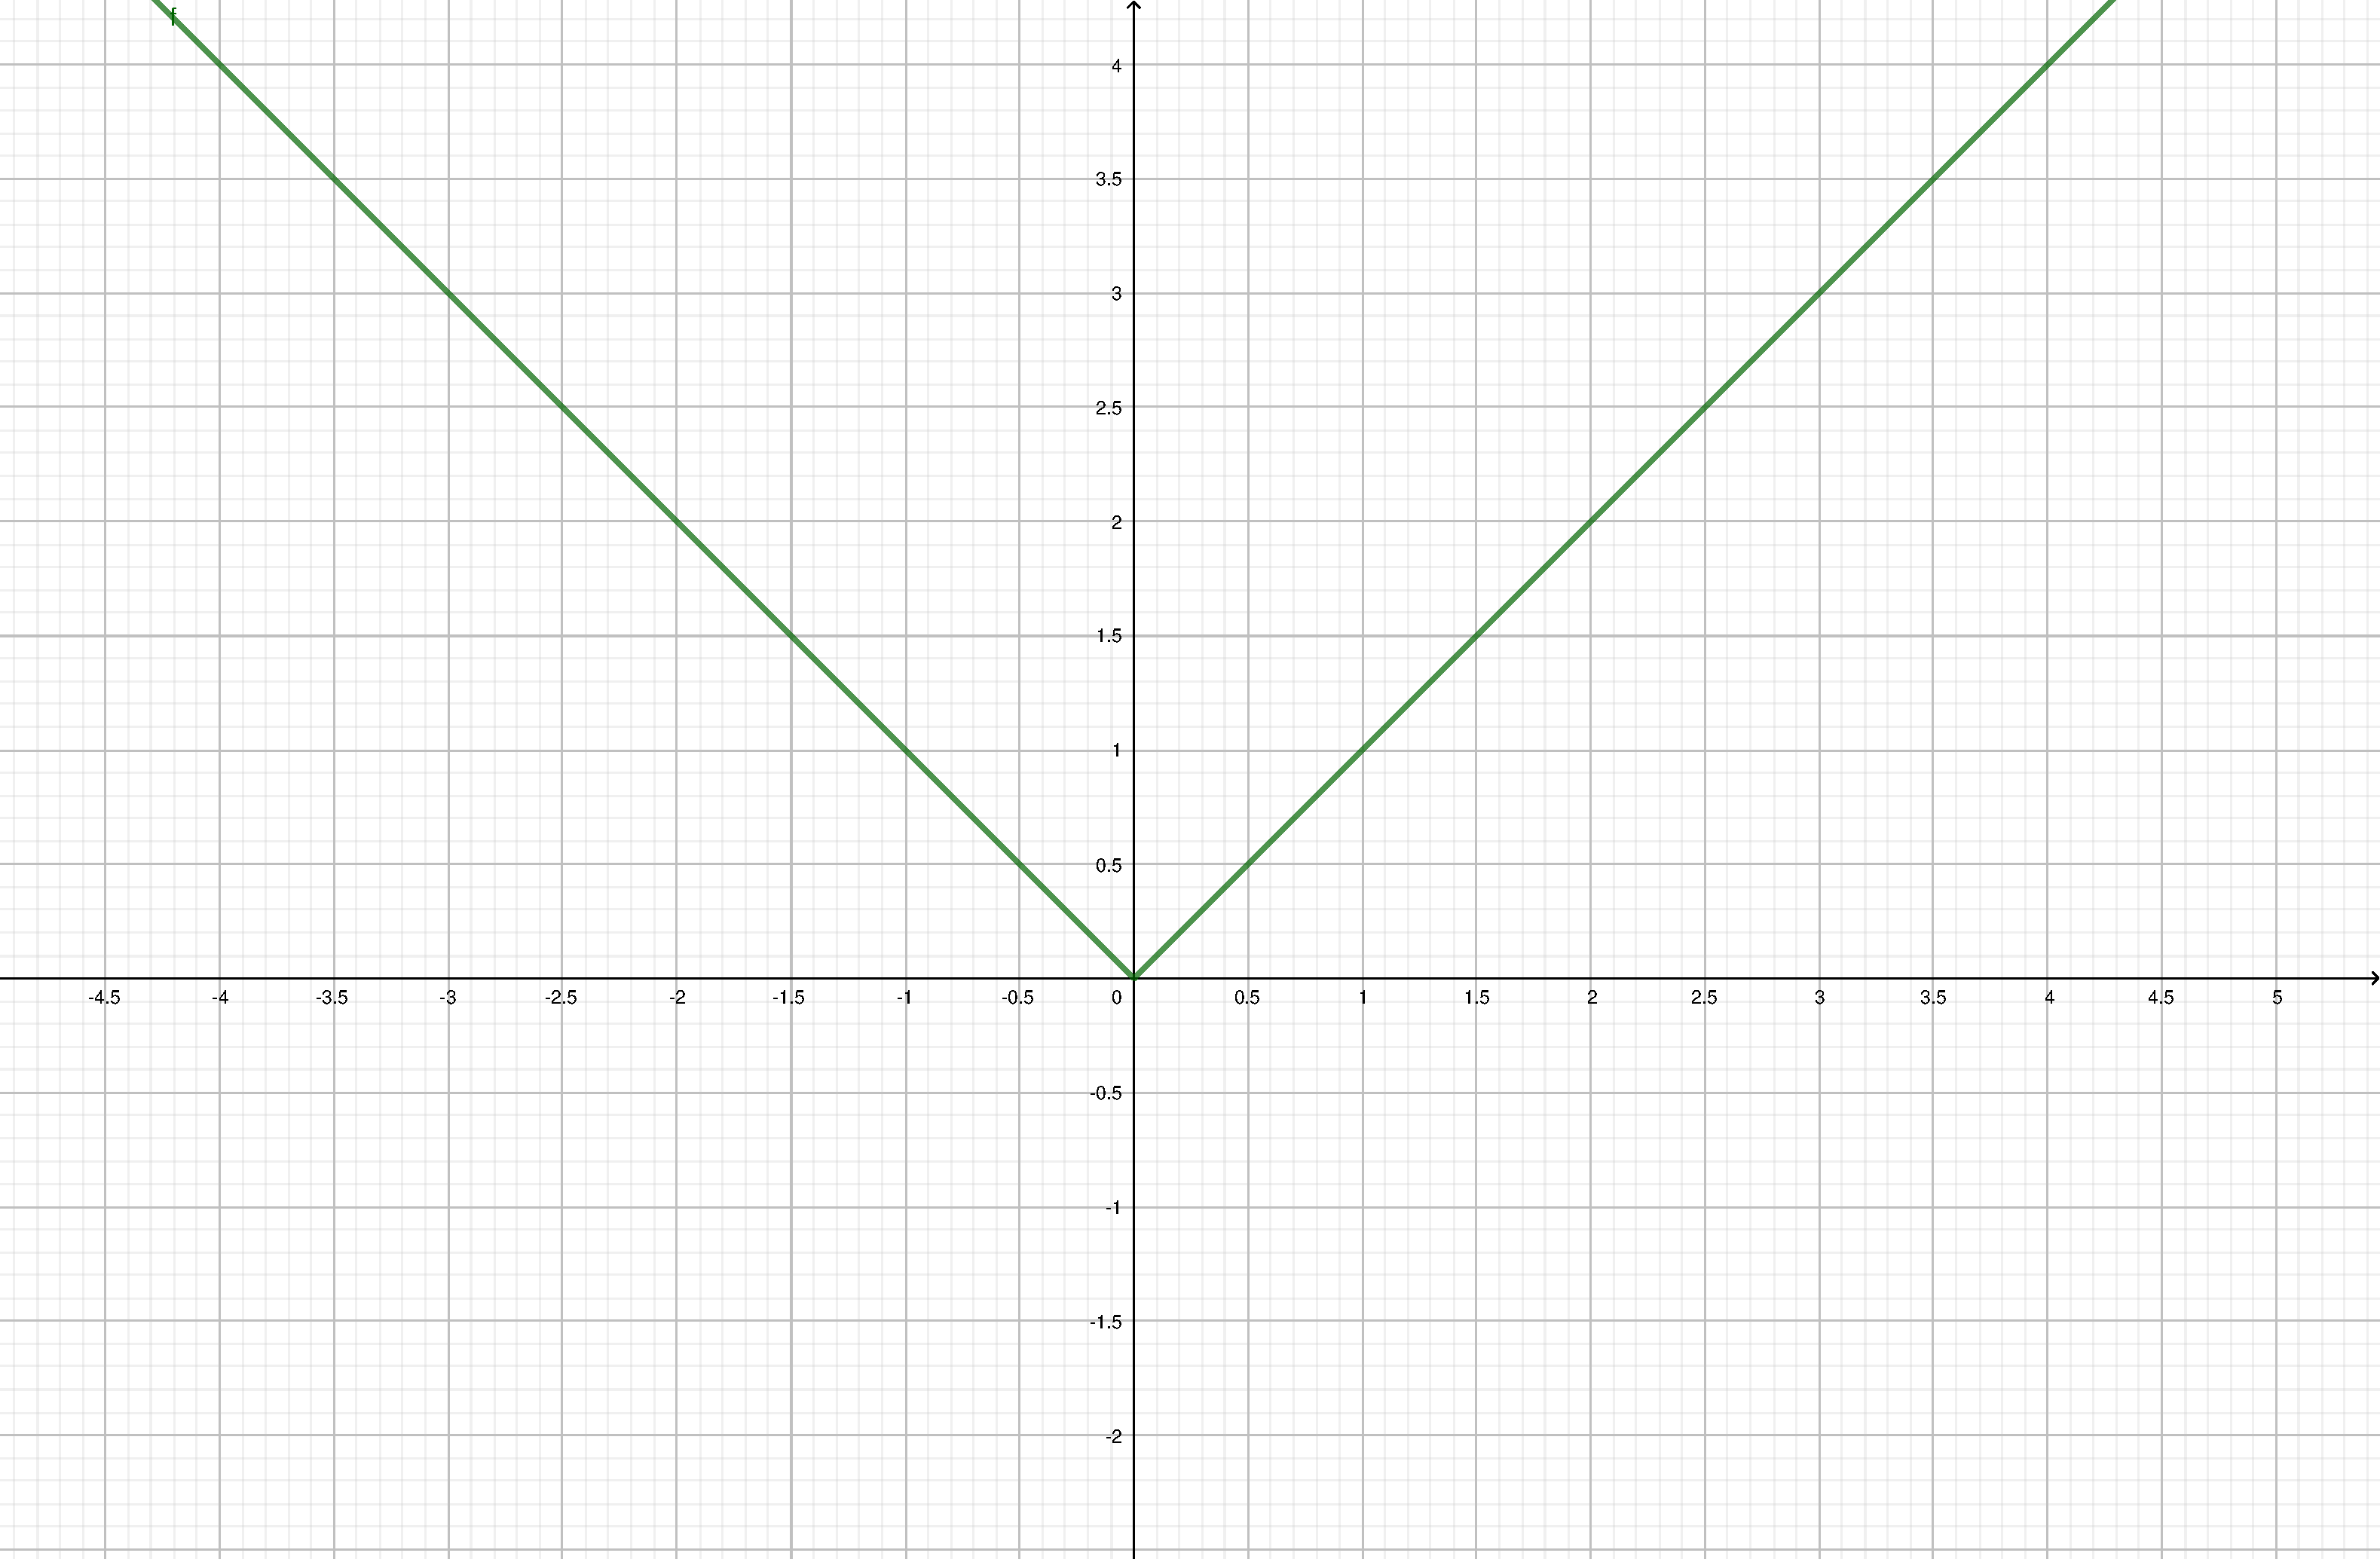
\includegraphics[height=8cm]{img/funzione valore assoluto.pdf}};
	\end{tikzpicture}
	\caption{Grafico di Funzione valore assoluto $y=|x|$}
\end{figure}
$C.E. \equiv R\text{ Limitata inferiormente in } x=0$\\
$|x|=\begin{cases}
	x&x\geq0\\
	-x& x<0
\end{cases}$
\subsection{Funzione potenza $y=x^n,n\in N, pari$}
\begin{figure}[!ht]
	\centering
	\begin{tikzpicture}
		\node[] (pic) at (0,0) {\includegraphics[height=8cm]{img/funzione
		potenziale x^n.pdf}};
	\end{tikzpicture}
	\caption{Grafico di Funzione potenza $y=x^n,n\in N, pari$}
\end{figure}\newpage
\subsection{Funzione potenza $y=x^\alpha,\alpha \in R$ (\textit{ma non
razionale})}
\begin{figure}[!ht]
	\centering
	\begin{tikzpicture}
		\node[] (pic) at (0,0) {\includegraphics[height=8cm]{img/funzione
		potenziale x^a.pdf}};
	\end{tikzpicture}
	\caption{Grafico di Funzione potenza $y=x^\alpha,\alpha \in R$ (\textit{ma non
razionale})}
\end{figure}
$C.E.:\{x\in R: x\geq 0\}$ Limitata inferiormente da $x=0$ non limitata
superiormente Strettamente crescente
\subsection{Funzione potenziale $y=x^{\frac{m}{n}},m, n\in Z$}
\begin{figure}[!ht]
	\centering
	\begin{tikzpicture}
		\node[] (pic) at (0,0) {\includegraphics[height=8cm]{img/funzione
		potenziale fratta.pdf}};
	\end{tikzpicture}
	\caption{Grafico di Funzione potenza $y=x^\alpha,\alpha \in R$ (\textit{ma non
razionale})}
\end{figure}
\subsection{Funzione logaritmo $y=\log_a{x}$}
\begin{figure}[!ht]
	\centering
	\begin{tikzpicture}
		\node[] (pic) at (0,0) {\includegraphics[height=8cm]{img/funzione
		logaritmica.pdf}};
	\end{tikzpicture}
	\caption{Funzione logaritmo $y=\log_a{x}$}
\end{figure}
$C.E.\equiv x>0$ Non limitata, strettamente crescente se $a>1$, Strettamente
decrescente se $0<a<1$.\newpage
\subsection{Le coniche: la circonferenza}
\begin{figure}[!ht]
	\centering
	\begin{tikzpicture}
		\node[] (pic) at (0,0) {\includegraphics[height=8cm]{img/le coniche
		circonferenze.pdf}};
	\end{tikzpicture}
	\caption{Le coniche: la circonferenza}
\end{figure}\newpage
\subsection{Le coniche: l'ellisse}
\begin{figure}[!ht]
	\centering
	\begin{tikzpicture}
		\node[] (pic) at (0,0) {\includegraphics[height=8cm]{img/le coniche
		ellisse.pdf}};
	\end{tikzpicture}
	\caption{Le coniche: l'ellisse}
\end{figure}
\subsection{Le coniche: iperbole}
\begin{figure}[!ht]
	\centering
	\begin{tikzpicture}
		\node[] (pic) at (0,0) {\includegraphics[height=8cm]{img/le coniche
		iperbole.pdf}};
	\end{tikzpicture}
	\caption{Le coniche: iperbole}
\end{figure}\newpage
\subsection{Le coniche: iperbole equilattera}
\begin{figure}[!ht]
	\centering
	\begin{tikzpicture}
		\node[] (pic) at (0,0) {\includegraphics[height=8cm]{img/le coniche
		iperbole equilattera.pdf}};
	\end{tikzpicture}
	\caption{Le coniche: iperbole equilattera}
\end{figure}
\subsection{Le coniche: parabola}
\begin{figure}[!ht]
	\centering
	\begin{tikzpicture}
		\node[] (pic) at (0,0) {\includegraphics[height=8cm]{img/le coniche
		parabola.pdf}};
	\end{tikzpicture}
	\caption{Le coniche: parabola}
\end{figure}\newpage
\subsection{Le funzioni trigonometriche}
Funzioni trigonometriche elementati:
$y=\sin x, y=cos x, y=\tan x, y=\cot x$\\
\textit{Relazioni fondamentali:} $(\sin x)^2+(\cos x)^2=1$, $\tan x=\frac{\sin
x}{\cos x}$, $\cot x=\frac{\cos x}{\sin x}$
\begin{figure}[!ht]
	\centering
	\begin{tikzpicture}
		\node[] (pic) at (0,0) {\includegraphics[height=8cm]{img/funzioni
		trigonometriche.pdf}};
	\end{tikzpicture}
	\caption{Le funzioni trigonometriche}
\end{figure}
\subsubsection{Funzione $\sin x$}
\begin{figure}[!ht]
	\centering
	\begin{tikzpicture}
		\node[] (pic) at (0,0) {\includegraphics[height=8cm]{img/funzione
		sin.pdf}};
	\end{tikzpicture}
	\caption{Funzione $\sin x$}
\end{figure}\newpage
\subsubsection{Funzione $\cos x$}
\begin{figure}[!ht]
	\centering
	\begin{tikzpicture}
		\node[] (pic) at (0,0) {\includegraphics[height=8cm]{img/funzione
		cos.pdf}};
	\end{tikzpicture}
	\caption{Funzione $\cos x$}
\end{figure}
\subsubsection{Funzione $\tan x$}
\begin{figure}[!ht]
	\centering
	\begin{tikzpicture}
		\node[] (pic) at (0,0) {\includegraphics[height=8cm]{img/funzione
		tg.pdf}};
	\end{tikzpicture}
	\caption{Funzione $\tan x$}
\end{figure}\newpage
\subsubsection{Funzione $\cot x$}
\begin{figure}[!ht]
	\centering
	\begin{tikzpicture}
		\node[] (pic) at (0,0) {\includegraphics[height=8cm]{img/funzione
		ctg.pdf}};
	\end{tikzpicture}
	\caption{Funzione $\cot x$}
\end{figure}
\subsection{Le funzioni trigonometriche inverse}
\subsubsection{Funzione $\arcsin x$}
\begin{figure}[!ht]
	\centering
	\begin{tikzpicture}
		\node[] (pic) at (0,0) {\includegraphics[height=8cm]{img/funzione
		arcsin.pdf}};
	\end{tikzpicture}
	\caption{Funzione $\arcsin x$}
\end{figure}\newpage
\subsubsection{Funzione $\arccos x$}
\begin{figure}[!ht]
	\centering
	\begin{tikzpicture}
		\node[] (pic) at (0,0) {\includegraphics[height=8cm]{img/funzione
		arccos.pdf}};
	\end{tikzpicture}
	\caption{Funzione $\arccos x$}
\end{figure}
\subsubsection{Funzione $\arctan x$}
\begin{figure}[!ht]
	\centering
	\begin{tikzpicture}
		\node[] (pic) at (0,0) {\includegraphics[height=8cm]{img/funzione
		arctg.pdf}};
	\end{tikzpicture}
	\caption{Funzione $\arctan x$}
\end{figure}\newpage
\subsubsection{Operazione sul grafico: traslazione della asse X}
\begin{figure}[!ht]
	\centering
	\begin{tikzpicture}
		\node[] (pic) at (0,0) {\includegraphics[height=8cm]{img/operazione sul
		grafico traslazione della asse x.pdf}};
	\end{tikzpicture}
	\caption{Operazione sul grafico: traslazione della asse X}
\end{figure}
\subsubsection{Operazione sul grafico: traslazione della asse Y}
\begin{figure}[!ht]
	\centering
	\begin{tikzpicture}
		\node[] (pic) at (0,0) {\includegraphics[height=8cm]{img/operazione sul
		grafico traslazione della asse y.pdf}};
	\end{tikzpicture}
	\caption{Operazione sul grafico: traslazione della asse Y}
\end{figure}\newpage
\subsubsection{Operazione sul grafico: contrazione e dilatazione in direzione verticale}
\begin{figure}[!ht]
	\centering
	\begin{tikzpicture}
		\node[] (pic) at (0,0) {\includegraphics[height=8cm]{img/contrazione e
		dilatazione in direzione verticale.pdf}};
	\end{tikzpicture}
	\caption{Operazione sul grafico: contrazione e dilatazione in direzione verticale}
\end{figure}
\subsubsection{Operazione sul grafico: contrazione e dilatazione in direzione
orizzontale}
\begin{figure}[!ht]
	\centering
	\begin{tikzpicture}
		\node[] (pic) at (0,0) {\includegraphics[height=8cm]{img/compressione e
		dilatazione in direzione orizzontale.pdf}};
	\end{tikzpicture}
	\caption{Operazione sul grafico: contrazione e dilatazione in direzione
	orizzontale}
\end{figure}\newpage
\subsubsection{Operazione sul grafico: $y=|f(x)|$}
\begin{figure}[!ht]
	\centering
	\begin{tikzpicture}
		\node[] (pic) at (0,0) {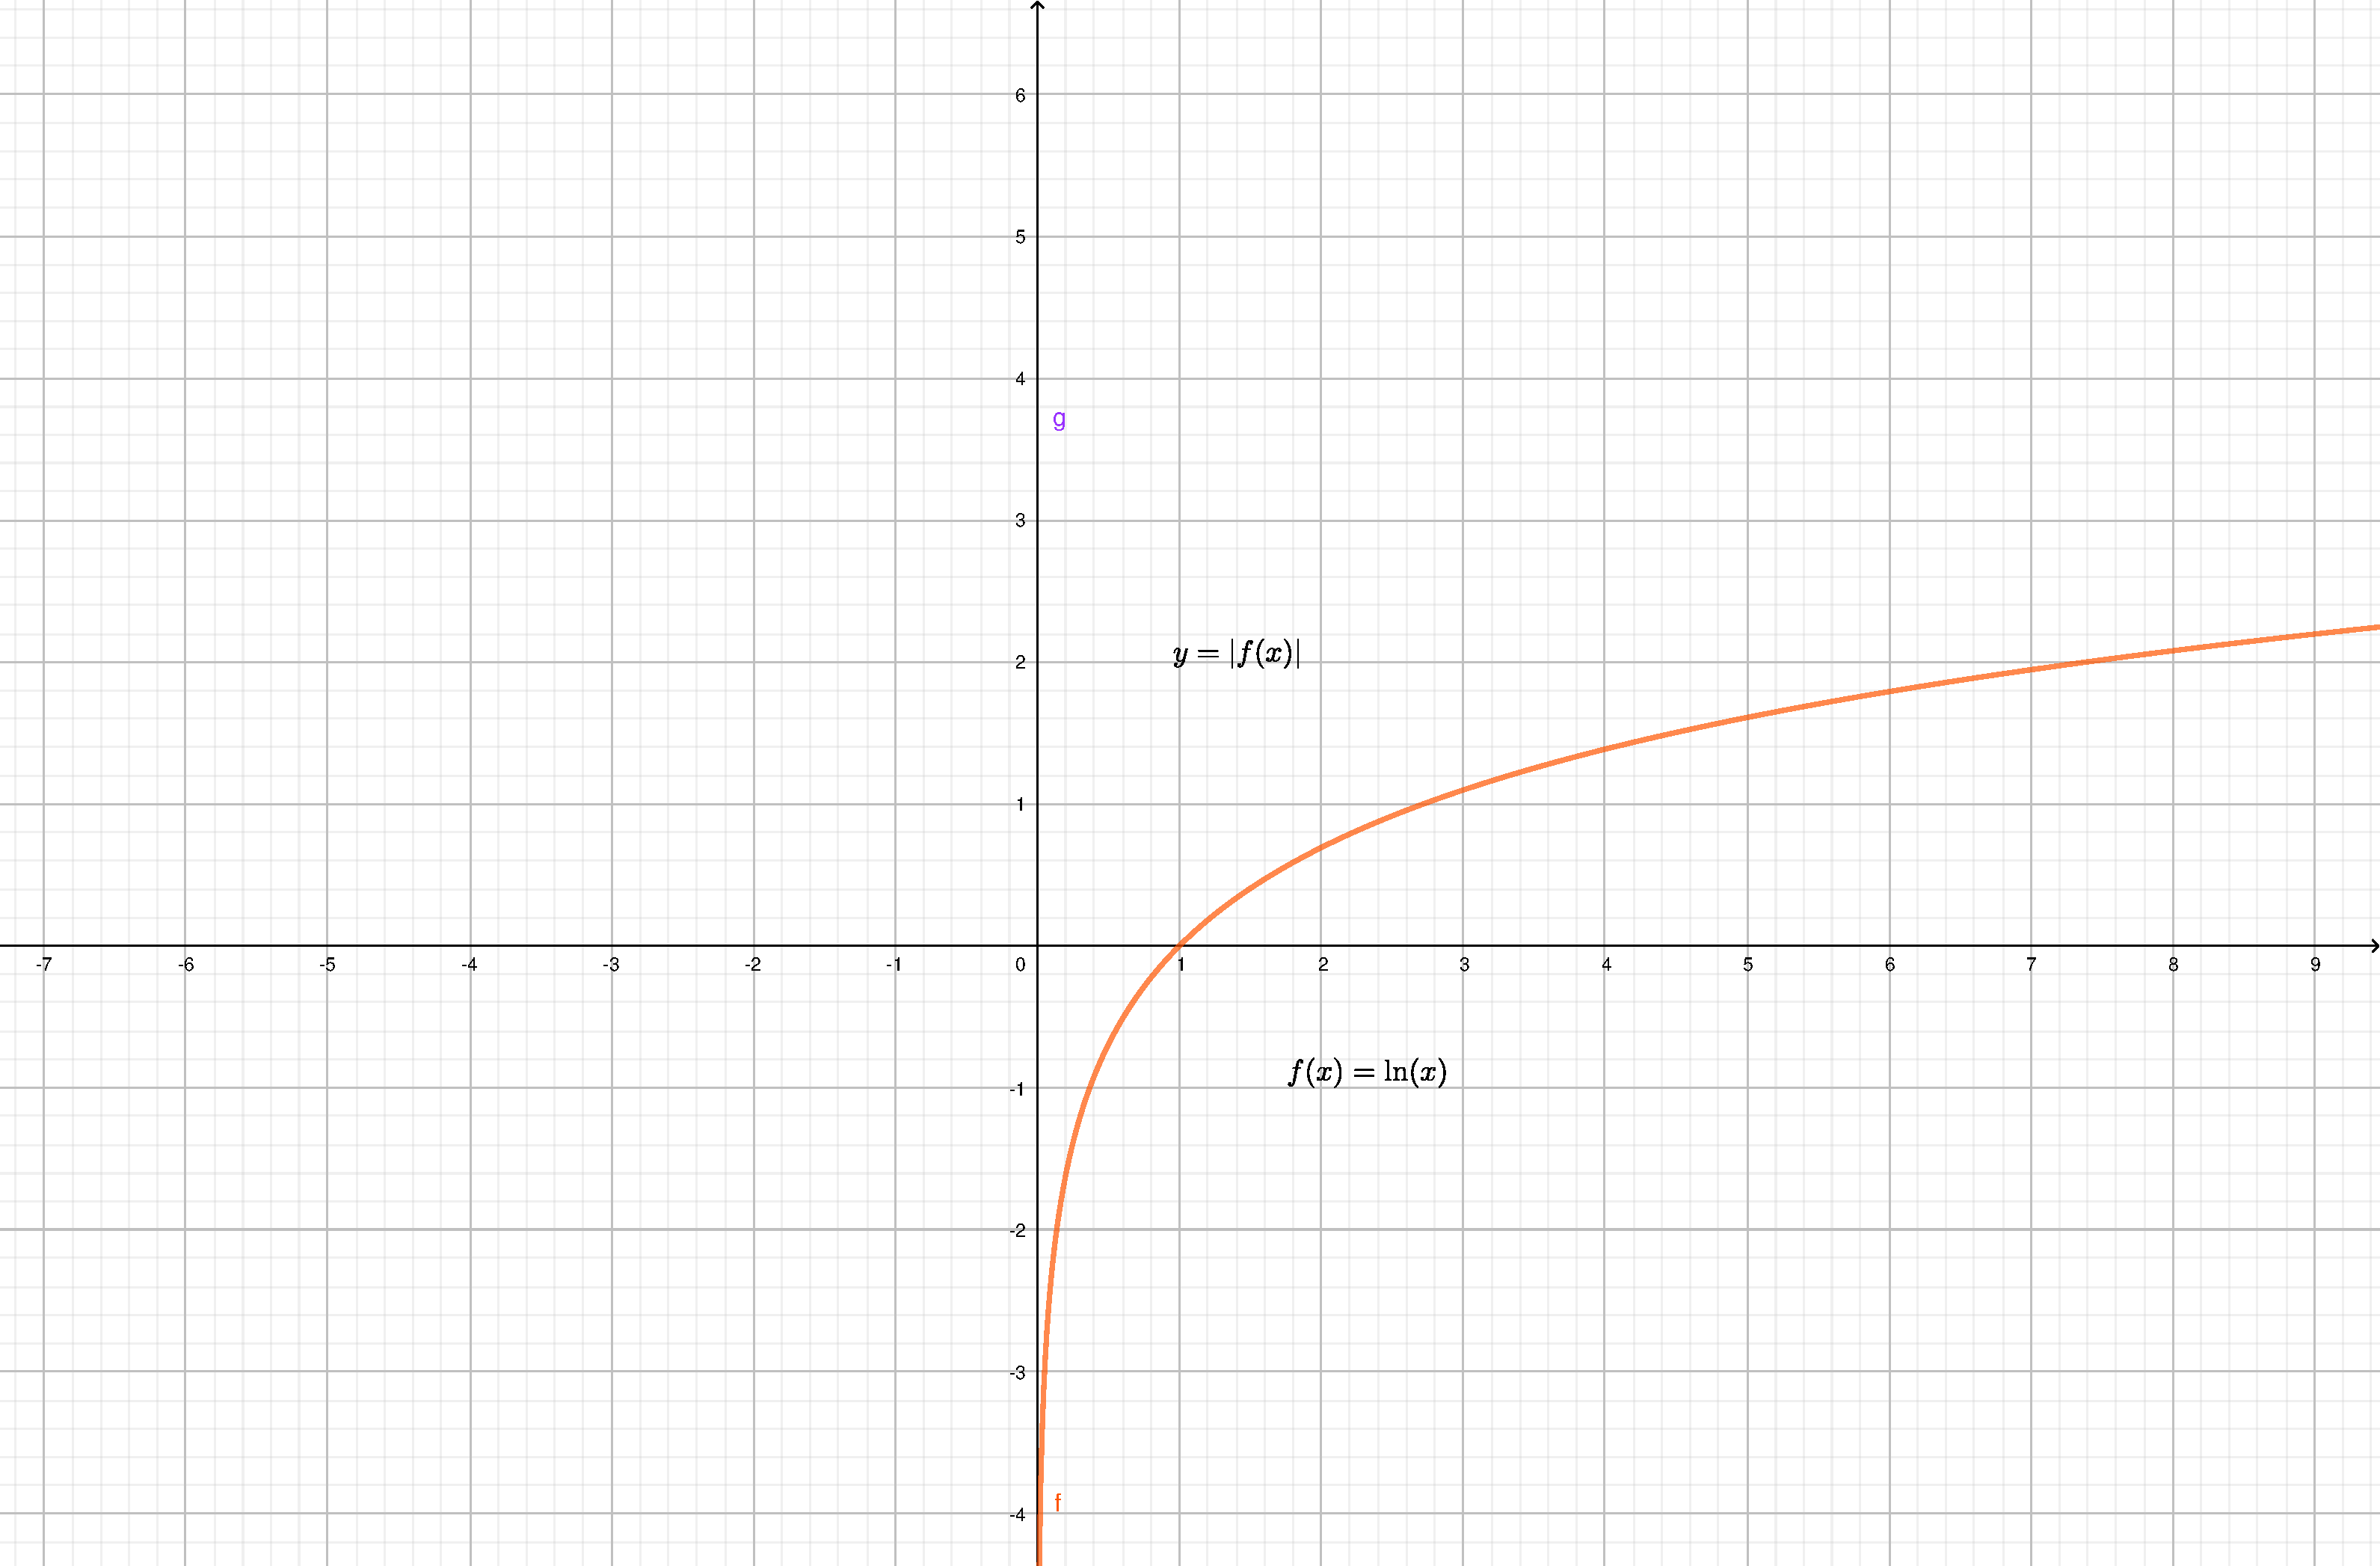
\includegraphics[height=8cm]{img/y=_lnx_.pdf}};
	\end{tikzpicture}
	\caption{Operazione sul grafico: $y=|f(x)|$}
\end{figure}

% passaggio ai limiti

\section{Limiti}
\begin{figure}[!ht]
	\centering
	\begin{tikzpicture}
		\node[] (pic) at (0,0) {\includegraphics[height=8cm]{img/esempio limite
		di funzione.pdf}};
	\end{tikzpicture}
	\begin{tabular}{|l|l|}
		\hline
		x&f(x)\\\hline\hline
		0,1& 0,998\\
		0,001&0,999\\\hline
	\end{tabular}
	$C.E.=R\textbackslash{}\{0\}$
	\caption{Esempio limite di funzione}
\end{figure}
Il limite di una funzione è un operazione, o meglio un operatore, che permette
di studiare il comportamento di una funzione nell'intorno di un punto $x_0$.\\
\textit{Mediamente il limite è possibile stabilire a quale valore tende la
funzione man mano che i valori della variabile si approssimano al punto $x_0$}.
\begin{figure}[!ht]
	\centering
	\begin{tikzpicture}
		\node[] (pic) at (0,0) {\includegraphics[height=8cm]{img/esempio di
		limite di una funzione.pdf}};
	\end{tikzpicture}
	\caption{Esempio di limite di una funzione}
\end{figure}
\subsection{Limite di una funzione}
Sia $f(x)$ definita in $A\in R$, e sia $x_0$ un punto di accumulazione per A.
Si dice che $f(x)$ ha limite $l$ per $x$ che tende a $x_0$, se $V\varepsilon
>0 \exists \delta_\varepsilon > 0: |f(x)-l|=\varepsilon\Rightarrow x\in
I(x_0,\delta_\varepsilon) \text{ escluso al più } x_0 \text{ cioè }
|x-x_0|<\delta_\varepsilon$
\begin{itemize}
	\item $l-\varepsilon < f(x) < l+\varepsilon$
	\item $x_0-\varepsilon < x<x_0+\delta_\varepsilon$
\end{itemize}
\subsubsection{In simboli}
$\lim_{x\to x_0} f(x)=l \text{   } f(x)\xrightarrow{x\to x_0} l$ 
\subsection{Definizione di Limite destro}
$l_1$ si definisce \textit{limite destro} di $f(x)$ per x che tende a $x_0^+$: $\lim_{x\to x_0^+ f(x)=l_1}$\\
se $\forall \varepsilon > 0 \exists \delta_\varepsilon>0 :
|f(x)-l_1|<\varepsilon\Rightarrow x_0<x<x_0+\delta_\varepsilon \text{ cioè }
x\in(x_0,x_0+\delta_\varepsilon)$
\subsection{Definizione di limite sinistro ``da sinistra''}
$l_2$ si definisce \textit{limite sinistro} di $f(x)$ per \textit{x} che tende
a $x^-_0$: $\lim_{x\to x_0^-}f(x)=l^2$ se $\forall \varepsilon>0 \exists
\delta_\varepsilon>0: |f(x)-l_2|<\varepsilon\Rightarrow
x_0-\delta_\varepsilon<x<x_0$ cioè $x\in(x_0-\delta_\varepsilon,x_0)$
\subsection{Teorema d'unicità del limite ``da destra''\label{dadestra}}
Se $\lim_{x\to x_0} f(x)=l\Rightarrow \text{l è unico}$\\
Dimostrazione. Per assurdo: supponiamo che $\exists l_1,l_2: l_1 \neq l_2$
con $l_1=lim_{x\to x_0}f(x)$ in $I(x_0,\delta_{1\varepsilon})$, $l_2=lim_{x\to
x_0}f(x)$ in $I(x_0,\delta_{2\varepsilon})$\\
Fissato $\varepsilon=\frac{|l_1-l_2|}{2}$\\
$2\varepsilon=|l_1-l_2|=|l_1-f(x)+f(x)-l_2|\leq|f(x)-l_2|+|f(x)-l_2|<2\varepsilon$
in $I(x_0,\delta_{\varepsilon})$,
$\delta_{\varepsilon}=min(\delta_{1\varepsilon},\delta_{2\varepsilon})$
Assurdo! $\Rightarrow l_1=l_2$
\subsubsection{Esempi}
\begin{tabular}{lc}
	$y=\frac{|x|}{x}$ & $C.E. = R\textbackslash \{0\}$\\
	$\lim_{x\to 0^+}\frac{|x|}{x}=1$&\multirow{2}{*}{$\nexists \text{ limitate}$} \\
	$\lim_{x\to 0^-}\frac{|x|}{x}=-1$&\\
\end{tabular}
\paragraph{Definizione} Sia $f(x)$ definita in $A \in R$, e sia $x_0$ un punto
di accumulazione per A. Si dice che $f(x)$ ha limite $+\infty$ per x che tende
a $x_0$, se $\forall M>0,\exists \delta_M>0:\forall x \in
I(x_0,\delta_m)\Rightarrow f(x)>M$

\fbox{
	\addtolength{\linewidth}{-2\fboxsep}%
	\addtolength{\linewidth}{-2\fboxrule}%
	\begin{minipage}{\linewidth}
 		\begin{equation}
   			\lim_{x\to x_0}f(x)=+\infty
 		\end{equation}
 	\end{minipage}
}
\paragraph{Definizione} Sia $f(x)$ definita in $A\in R$, e sia $x_0$ un punto
di accumulazione per A. Si dice che $f(x)$ ha limite $-\infty$ per $x$ che
tende a $x_0$, se $\forall M>0, \exists \delta_M>0:\forall x \in
I(x_0,\delta_m)$
risulta $f(x)<-M$.

\fbox{
	\addtolength{\linewidth}{-2\fboxsep}%
	\addtolength{\linewidth}{-2\fboxrule}%
	\begin{minipage}{\linewidth}
 		\begin{equation}
   			\lim_{x\to x_0}f(x)=-\infty
 		\end{equation}
 	\end{minipage}
}

\paragraph{Definizione di Asintoto verticale}
Se $\boxed{\lim_{x\to x_0}f(x)=\infty}$ allora la retta verticale $\boxed{x=x_0}$
si chiama asintoto verticale
\begin{figure}[!ht]
	\centering
	\begin{tikzpicture}
		\node[] (pic) at (0,0) {\includegraphics[height=8cm]{img/asintoto
		verticale.pdf}};
	\end{tikzpicture}
	\caption{Asintoto verticale}
\end{figure}\\
Sia $f(x)$ definita in $A\in R$, si dice che $f(x)$ ha limite $l$, per $x$ che
tende a $+\infty$, se: $\forall_\varepsilon>0, \exists K_\varepsilon >0:\forall
x \in I (K_\varepsilon, +\infty)$ risulta $|f(x)-l|<\varepsilon$
\begin{equation*}
	\boxed{\lim_{x\to+\infty}f(x)=l}
\end{equation*}
\newpage
\paragraph{Definizione di Asintoto orizzontale} Se \begin{tabular}{|l|}
	\hline
	$\lim_{x\to \infty}f(x)=l$\\\hline
\end{tabular} Allora la retta orizzontale $\boxed{y=l}$ si chiama Asintoto orizzontale
\begin{figure}[!ht]
	\centering
	\begin{tikzpicture}
		\node[] (pic) at (0,0) {\includegraphics[height=8cm]{img/asintoto
		orizzontale.pdf}};
	\end{tikzpicture}
	\caption{Asintoto orizzontale}
\end{figure}\\
Sia $f(x)$ definita in $A \in R$, si dice che $f(x)$ ha limite $+\infty$, per x
che tende a $+\infty$, se: $\forall M>0, \exists K_M >0: \forall x \in (K_M,
+\infty)$ risulta $f(x)\in (M,+\infty)$ \begin{tabular}{|l|}
	$\lim_{x\to +\infty}f(x) = +\infty$
\end{tabular}
\subsection{Teorema (\texttt{\color{red} algebra dei limiti})}
Se:
\begin{itemize}
	\item $\lim_{x\to x_0} f(x)=l_1$ $\lim_{x\to x_0} g(x) = l_2$
	\item $\lim_{x\to x_0} f(x)\pm g(x)=l_1\pm l_2$
	\item $\lim_{x\to x_0} f(x)*g(x)=l_1*l_2$
	\item $\lim_{x\to x_0} \frac{f(x)}{g(x)}=\frac{l_1}{l_2}, g(x), l_2\neq 0$

\end{itemize}
\subsection{Convenzioni con $\infty$}
\begin{itemize}
	\item $\forall a >0, a\pm \infty=\pm \infty$
	\item $+\infty+\infty=+\infty$
	\item $-\infty-\infty=-\infty$
	\item $\forall a> 0, a*(\pm \infty)=\pm \infty$
	\item $\forall b< 0, b*(\pm \infty)=\mp \infty$
	\item $(\pm\infty)*(\pm \infty)=+\infty$
	\item $(\pm\infty)*(\mp \infty)=-\infty$

\end{itemize}
\subsubsection{Convenzioni con $\infty$}
$\frac{a}{\infty}=0$ $\frac{a}{0}=\infty$

\subsection{Forme indeterminate}
\begin{tabular}{|llllllll|}
	\hline
	$+\infty-\infty$&$\frac{\infty}{\infty}$&$\frac{0}{0}$&$1^\infty$&$e^{+\infty*0}$&$0-\infty$&$0^0$&$0*\infty$\\
	\hline
\end{tabular}
\begin{itemize}
	\item 
	\begin{equation*}
		a^{+\infty}=\begin{cases}
			+\infty,&a>1\\
			0,&0<a<1
		\end{cases}
	\end{equation*}
	\item 
	\begin{equation*}
		a^{-\infty}=\begin{cases}
			0,&a>1\\
			+\infty,&0<a<1
		\end{cases}
	\end{equation*}
\end{itemize}
\subsubsection{Come si risolvono?}
\begin{description}
	\item [$\frac{\infty}{\infty}$ e $\frac{0}{0}$ ] Il limite che andremo a studiare è
	
	\fbox{
 		\addtolength{\linewidth}{-2\fboxsep}%
		\addtolength{\linewidth}{-2\fboxrule}%
		\begin{minipage}{\linewidth}
 			\begin{equation}
				\lim_{x\to 0} \frac{\arctan{x}}{\ln{(1+x)}}  \text{ forma ineterinata}
 			\end{equation}
		\end{minipage}
	}
	In questo caso possiamo applicare la regola di \underline{de l'Hopital} [\ref{del'hop}], che ci consente di eseguire il calcolo in modo abbastanza rapido, consiste nel derivare singolarmente il \textbf{numeratore} e il \textbf{denominatore} e in questo caso il risultato sarà $\arctan x=\frac{1}{1+x^2}$ e $\ln{(1+x)}=\frac{1}{1+x}$, adesso rimettiamo assieme il limite di prima e il risultato è questo:
	\begin{equation*}
		\lim_{x\to 0}\bigg[\frac{\big(\frac{1}{1+x^2}\big)}{\big(\frac{1}{1+x}\big)}\bigg]
	\end{equation*}
	Ovviamente in questo caso conviene utilizzare le regole delle frazioni per renderci il lavoro più semplice, quindi, lo esprimiamo sotto forma di moltiplicazione e il risultato è il seguente:
	 \begin{equation*}
		\lim_{x\to0} \bigg[\frac{1}{1+x^2}*(1+x)\bigg]=\frac{1}{1+0}*(1)=1
	\end{equation*}
	Ed ecco che adesso il limite assume un valore determinato.
	\item[$+\infty-\infty$ ] Il limite che andremo a studiare è
		\begin{equation*}
			\lim_{x\to\infty} \big(\sqrt{x^2+x}-\sqrt{x^2-x}\big)=\infty-\infty
		\end{equation*}
		In questo caso va per forza di cose razionalizzato
		\begin{equation*}
			\lim_{x\to\infty}\frac{(\sqrt{x^2+x}-\sqrt{x^2-x})(\sqrt{x^2+x}+\sqrt{x^2-x})}{\sqrt{x^2+x}+\sqrt{x^2-x}}=\lim_{x\to\infty}\bigg[\frac{(x^2+x)-(x^2)}{\sqrt{x^2+x}+\sqrt{x^2-x}} \bigg]=\lim_{x\to\infty}\frac{\not{x^2}+x-\not{x^2}+x}{\sqrt{x^2+x}+\sqrt{x^2-x}}
		\end{equation*}
		\begin{equation*}
			\lim_{x\to\infty}\frac{2x}{\sqrt{x^2+x}+\sqrt{x^2-x}}=\frac{\infty}{\infty}
		\end{equation*}
		Ovviamente una volta che otteniamo questa forma indeterminata, possiamo proseguire con la regola di de l’Hopital [\ref{del'hop}] che è valida solo per due casi di indeterminazione: $\frac{0}{0}$ e $\frac{\infty}{\infty}$, quindi deriviamo numeratore e denominatore singolarmente e il risultato è il seguente:
		\begin{equation*}
			\lim_{x\to \infty}\frac{2}{\frac{1}{2\sqrt{x^2+x}}*(2x+1)+\frac{1}{2\sqrt{x^2-x}}*(2x-1)}=\frac{2}{1+1}=\frac{\not{2}}{\not{2}}=1
		\end{equation*}
		Ed ecco che il limite assume un valore determinato\dots Nel modo più semplice e indoloro possibile.
	\item [$0*\infty$ ] Il limite che adesso studieremo è
		\begin{equation*}
			\lim_{x\to 0}[x*e^\frac{1}{x}]=0*e^\infty=0*\infty=\text{ forma indeterminata}
		\end{equation*}
		Ovviamente in questa forma non è molto comoda da studiare quindi, bisogna scriverla in questo modo, per poterla studiare con il metodo di \underline{de l'Hopital}.
		\begin{equation*}
			\lim_{x\to 0}\bigg[\frac{e^\frac{1}{x}}{\frac{1}{x^2}}\bigg]
		\end{equation*}
		Quindi dopo aver sfruttato le proprietà delle frazioni, perché ovviamente $x*e^\frac{1}{x}=\frac{e^\frac{1}{x}}{\frac{1}{x}}$, dopo averla in questo modo possiamo applichiamo la regola di  \underline{de l'Hopital} [\ref{del'hop}], Quindi procediamo come nel precedente caso ``$+\infty-\infty$''
		\begin{equation*}
			\lim_{x\to 0}\bigg[\frac{e^\frac{1}{x}*(-\frac{1}{x^2})}{(-\frac{1}{x^2})}\bigg]=\lim_{x\to 0}e^\frac{1}{x}=e^\frac{1}{0^+}=e^\infty=\infty
		\end{equation*}
		E adesso da un valore determinato.
	\item [$0^0$ ] Il limite che andiamo a studiare in questo caso è
		
		\fbox{
 			\addtolength{\linewidth}{-2\fboxsep}%
 			\addtolength{\linewidth}{-2\fboxrule}%
 			\begin{minipage}{\linewidth}
  				\begin{equation}
   					\lim_{x\to 0}x^x=0^0 \text{ 	forma ineterinata}
  				\end{equation}
 			\end{minipage}
		}
		In questo caso bisogna procedere in questo modo:
		\begin{equation*}
			x^x=e^{\ln{x^x}}=e^{{x*\ln x}}=e^\frac{\ln x}{\frac{1}{x}}
		\end{equation*}
		In definitiva bisogna procedere con regola di \underline{de l'Hopital} [\ref{del'hop}] e lo svolgimento sarà il seguente
		\begin{equation*}
			\lim_{x\to 0^+}e^\frac{\ln x}{x}=\lim_{x\to 0^+}e^{\bigg(\frac{\frac{1}{x}}{-\frac{1}{x}}\bigg)}=\lim_{x\to 0^+}e^{-x}=e^0=1
		\end{equation*}
		Ovviamente essendo un logaritmo si prende solo lo $0^+$ ``da destra'' [\ref{dadestra}], anche in questo caso alla fine ha reso un valore determinato.
\end{description}
\fbox{
 	\addtolength{\linewidth}{-2\fboxsep}%
 	\addtolength{\linewidth}{-2\fboxrule}%
 	\begin{minipage}{\linewidth}
		\paragraph{Consiglio:} Utilizza sempre le parentesi per isolare le parti e evitare inutili confusioni, indica da che parte stai studiano il limite solo dove è rilevante e esegui tutti i passaggi se ci sono dubbi, perché non bisogna mai sottovalutare quello che viene chiesto dall'esercizio, perché può essere abbastanza insidioso e anche una vera e propria trappola che serve a provare il livello della comprensione del testo del candidato.
	\end{minipage}
}
\subsection{Teorema del confronto}
Siano $f(x)\text{ },f_1(x)\text{ },f_2(x)$ tre funzioni definite in $A\subseteq R$ sia $x_0$ un
punto di accumulazione per A e $f_1(x)\leq f(x) \leq f_2(x)$ se $\lim_{x\to
x_0}f_1(x)=\lim_{x\to x_0} f_2(x)=l$ allora $\lim_{x\to x_0} f(x)=l$
\subsubsection{Dimostrazione}
Se $\lim_{x\to x_0} f_1(x)=\lim_{x\to x_0} f_2(x)=l$ allora per definizione di
limite:
\begin{itemize}
	\item $\exists \delta_1:|f_1(x)-l|<\varepsilon$ $\forall x \in I(x_0,\delta_1)$
	\item $\exists \delta_2:|f_2(x)-l|<\varepsilon$ $\forall x \in
		I(x_0,\delta_2)$
\end{itemize}
\begin{equation*}
	\Rightarrow l-\varepsilon < f_1(x) \leq f(x)\leq f_2(x) < l+ \varepsilon
\end{equation*}

$\forall x \in I(x_0,\delta_2), \delta = \min (\delta_1,\delta_2)$
\subsubsection{Casi particolari di $\lim_{x\to x_0} f(x)*g(x)$}
\paragraph{Teorema}
Se $\lim_{x\to x_0} f(x)=x$; $|g(x)|\leq M$ per $x\in I(x_0,\delta)\Rightarrow
\lim_{x\to x_0}f(x)*g(x)=0$
\subparagraph{Esempio} $\lim_{x\to x_0}x*\sin\frac{1}{x}=0$
\subsection{Limite di \texttt{funzione composta}}
Siano $g:A\to B:B\to R:$ $\lim_{x\to x_0}g(x)=y_0$ e $\lim_{y\to y_0}f(y)=l$
con $l=f(y_0)$ (\textit{se f è continua})\\
$\Rightarrow$\begin{tabular}{|l|}
	\hline$\lim_{x\to x_0}f[g(x)]=l$\\\hline
\end{tabular}
\subsection{Limiti Notevoli}
\subsubsection{esponenziali e logaritmici}
\begin{multicols}{2}
\begin{equation}
	\lim_{x\to\pm\infty}\left(1+\frac{1}{x}\right)^x=e
\end{equation}
\begin{equation}
	\lim_{x\to+\infty}\left(1+\frac{a}{x}\right)^x=e^a
\end{equation}
\begin{equation}
	\lim_{x\to+\infty}\left(1+\frac{a}{x}\right)^{nx}=e^{na}
\end{equation}
\begin{equation}
	\lim_{x\to-\infty}\left(1+\frac{a}{x}\right)^x=\frac{1}{e}
\end{equation}
\begin{equation}
	\lim_{x\to0}\left(1+ax\right)^{\frac{1}{x}}=e^{a}
\end{equation}
\begin{equation}
	\lim_{x\to0}\lg_a\left(1+x\right)^\frac{1}{x}=\frac{1}{\lg_e a}
\end{equation}
\begin{equation}
	\lim_{x\to0}\frac{\lg_a\left(1+x\right)}{x}=\lg_ae=\frac{1}{\ln a}
\end{equation}
\begin{equation}
	\lim_{x\to0}\frac{a^x-1}{x}=\ln a
\end{equation}
\begin{equation}
	\lim_{x\to0}\frac{\left(1+x\right)^a-1}{x}=a
\end{equation}
\begin{equation}
	\lim_{x\to0}\frac{\left(1+x\right)^a-1}{x}=1
\end{equation}
\begin{equation}
	\begin{matrix}
		\lim_{x\to0}x^r\lg_a x=0&\forall \in R^+-\{1\},&\forall r\in R^+
	\end{matrix}
\end{equation}
\begin{equation}
	\begin{matrix}
		\lim_{x\to0}\frac{\lg_a x}{x^r}=0&\forall \in R^+-\{1\},&\forall r\in R^+
	\end{matrix}
\end{equation}
\begin{equation}
	\lim_{x\to+\infty}x^ra^x=\lim_{x\to+\infty}a^x
\end{equation}
\begin{equation}
	\lim_{x\to-\infty}\abs{x}^ra^x=\lim_{x\to\infty}a^x
\end{equation}
\begin{equation}
	\begin{matrix}
		\lim_{x\to+\infty}\frac{e^x}{x^r}=\lim_{x\to+\infty}a^x&\forall r \in R^+
	\end{matrix}
\end{equation}
\begin{equation}
	\begin{matrix}
		\lim_{x\to+\infty}\frac{x^x}{e^r}=\lim_{x\to+\infty}a^x&\forall r \in R^+
	\end{matrix}
\end{equation}
\begin{equation}
	\begin{matrix}
		\lim_{x\to-\infty}e^x*x^r=0&\forall r \in R^+
	\end{matrix}
\end{equation}
\end{multicols}
\subsection{Goniometrici}
\begin{multicols}{2}
\begin{equation}
	\lim_{x\to0}\frac{\sin x}{x}=1
\end{equation}
\begin{equation}
	\lim_{x\to0}\frac{\sin ax}{bx}=\frac{a}{b}
\end{equation}
\begin{equation}
	\lim_{x\to0}\frac{\tan x}{x}=1
\end{equation}
\begin{equation}
	\lim_{x\to0}\frac{\tan ax}{bx}=\frac{a}{b}
\end{equation}
\begin{equation}
	\lim_{x\to0}\frac{1-\cos x}{x}=0
\end{equation}
\begin{equation}
	\lim_{x\to0}\frac{1-\cos x}{x^2}=\frac{1}{2}
\end{equation}
\begin{equation}
	\lim_{x\to0}\frac{\arcsin x}{x}=1
\end{equation}
\begin{equation}
	\lim_{x\to0}\frac{\arcsin ax}{bx}=\frac{a}{b}
\end{equation}
\begin{equation}
	\lim_{x\to0}\frac{arctan x}{x}=1
\end{equation}
\begin{equation}
	\lim_{x\to0}\frac{\arctan ax}{bx}=\frac{a}{b}
\end{equation}
\begin{equation}
	\lim_{x\to0}\frac{\sinh x}{x}=1
\end{equation}
\begin{equation}
	\lim_{x\to0}\frac{\mbox{settsinh}(x)}{x}=1
\end{equation}
\begin{equation}
	\lim_{x\to0}\frac{x-\sin x}{x^3}=\frac{1}{6}
\end{equation}
\begin{equation}
	\lim_{x\to0}\frac{x-\arctan x}{x^3}=\frac{1}{3}
\end{equation}
\end{multicols}
\paragraph{Esempi}
\begin{multicols}{2}
	\begin{enumerate}
		\item $\lim_{x\to x_0^+}xe^x+e^{-\frac{1}{x}}=0$
		\item $\lim_{x\to x_0^-}xe^x+e^{-\frac{1}{x}}=\infty$
		\item $\lim_{x\to x_0}\frac{1-\cos (x)}{x^2}=\lim_{x\to
			x_0}\frac{(1-\cos (x))(1+\cos (x))}{x^2(1+\cos x)}=\frac{1}{2}$
		\item $\lim_{x\to +\infty}\frac{1}{x}+\arctan{x}=\frac{\pi}{2}$
	\end{enumerate}
\end{multicols}
\begin{figure}[!ht]
	\centering
	\begin{tikzpicture}
		\node[] (pic) at (0,0) {\includegraphics[height=8cm]{img/esempio studio
		di funzione 2.pdf}};
	\end{tikzpicture}
	\caption{Esempio di limite notevole di una funzione}
\end{figure}

\subsection{Infinitesimi e infiniti}
\paragraph{Definizione}
Una funzione $f(x)$ su dice \underline{infinitesima} per $x\to x_0$ (per $x\to \infty$), $x_0$ punto di accumulazione per il dominio di $f(x)$, se: $\lim_{x\to x_0}f(x)=0$ (oppure $lim_{x\to \infty}f(x)=0$).
\subsubsection{Ordine di infinitesimo}
Siano $f(x)$ e $g(x)$ infinitesimi per $x\to{x_0}$ (o per $x\to \infty$), con $g(x)\neq 0$. Se $\exists\alpha R+$ e $l\in R$, $l\neq 0$ tale che\\
$\lim_{x\to{x_0}}=\frac{f(x)}{[g(x)]^\alpha}=l$ (oppure $\lim_{x\to{\infty}}=\frac{f(x)}{[g(x)]^\alpha}=l$)\\
Allora, si dice che per $x\to x_0$ (o per $x\to \infty$), $f(x)$ è un infinitesimo di ordine $\alpha$ rispetto all'infinitesimo campione $g(x)$.
\paragraph{Esempi}
\begin{itemize}
	\item $y=\sin{x}$ è un infinitesimo per $x\to 0$ di ordine 1 rispetto all'infinitesimo campione $g(x)=x$, infatti, $\lim_{x\to 0}=\frac{\sin{x}}{x^\alpha}=1$ solo se $\alpha = 1$
	\item $y=\tan^2x$ è un infinitesimo di ordine 2 rispetto ad x, per $x\to 0$
	\item $ord(1-\cos{x})=2$ rispetto ad $x$ per $x\to 0$
	\item La somma non varia l'ordine totale
	\item La moltiplicazione somma gli ordini
\end{itemize}
\subsubsection{Confronto tra infinitesimi}
Siano $f(x)$ e $g(x)$ infinitesime per $x\to x_{0}$,
\begin{equation}\label{Confronto tra infinitesimi}
	\lim_{x\to x_0}\frac{f(x)}{g(x)}=
	\begin{cases}
		l\neq 0&ord(f)=ord(g)\\
		\pm \infty&ord(f)<ord(g)\\
		0&ord(f)>ord(g)\\
		\text{non esiste,} & \text{f e g non confrontabile} \\ 
	\end{cases}	
\end{equation}

Stesso risultato se $f(x)$ e $g(x)$ sono infinitesime per $x\to \infty$. Utilizzando il confronto tra infinitesimi nel calcolo dei limiti del tipo $\lim_{x\to x_0}\frac{f_1+f_2}{g_1+g_2}$, dove $f_1,f_2,g_1,g_2$ sono funzioni infinitesime per $x\to x_0$, si possono {\color{blue} \em trascurare gli infinitesimi di ordine maggiore} (analogo discorso per funzioni infinitesime $x\to \infty$).
\subparagraph{esempio}
$\lim_{x\to 0}\frac{x^2+x^3+2\tan{x}}{(e^x-1)^2+\sin{x}}=\lim_{x\to 0}\frac{2\tan x}{\sin x}=2$
\paragraph{Definizione di funzioni asintotiche}
Si dice che due funzioni $f,g$ sono asintotiche per $x\to x_0$ se $\lim_{x\to x_0}\frac{f(x)}{g(x)}=1$ e si scrive $f\sim g$ per $x\to x_0$
\subparagraph{esempi}
\begin{itemize}
	\item $\sin x\sim x$ per $x\to 0$
	\item $\ln(1+x)\sim x$ per $x\to 0$
	\item $e^x-1\sim x$ per $x\to 0$ 
\end{itemize}
\paragraph{Definizione di funzioni infinite}
Una funzione $f(x)$ si dice \textit{infinita} per $x\to x_0$ (o per $x \to \infty$) , $x_0$ punto di accumulazione per il dominio di $f(x)$, (o per $x\to \infty$) se:
\begin {center}
	$\lim_{x\to x_0}f(x)=\infty$ (oppure $\lim_{x\to \infty}f(x)=\infty$)
\end{center}
\subparagraph{Esempi}
\begin{itemize}
	\item $y=e^x$ è un infinito per $x\to +\infty$
	\item $y=\ln{x}$ è un infinito per $x\to 0^+$
	\item $y=x^2+x$ è un infinito per $x\to \infty$
\end{itemize}
\subparagraph{Regole aritmetiche}
Siano $f(x)=o(x^\alpha)$ (si legge <<o piccolo di>>) e $g(x)=o(x^\beta)$ due funzioni \textit{infinitesime} rispettivamente di ordine $\alpha$ e $\beta$ per $x \to 0$ Allora si ha
\begin{itemize}
	\item $cf(x))o(x^\alpha)$, $\forall c \in R$
	\item $x^\lambda f(x)=o(x^{\lambda+\alpha})$
	\item $f(x)g(x)=o(x^{\alpha+\beta})$
	\item $f(x)+g(x)=o(x^y)$, $\gamma=\min(\alpha,\beta)$
\end{itemize}
\subsubsection{Esempi}
\begin{itemize}
	\item $y=e^x$ è un infinitesimo per $x\to -\infty$
	\item $y=\ln{x}$ è un infinitesimo per $x\to 1$
	\item $y=\sin{x}$ è un infinitesimo per $x\to 0$ (ma anche per $x\to \pi,2\pi$, etc.)
	\item $y=\ln{1+x}$ è un infinitesimo per $x\to 1$ 
\end{itemize}
\subsection*{definizione di infinitesimo}
$f(x)$ è un infinitesimo di ordine $\alpha$ se:
\begin{equation*}
	\lim_{x\to0}\frac{f(x)}{x^\alpha}=l
\end{equation*}
$x^\alpha$ = infinitesimo campione.
\subparagraph*{Esempio}
\begin{equation*}
	f(x)=\arcsin x^2 \text{ è un infinitesimo di ordine 2 perché}
\end{equation*}
\begin{equation*}
	\lim_{x\to 0}\frac{\arcsin x^2}{x^2}=\lim_{x\to 0}\frac{\frac{1}{1+x^4}*\not{2x}}{\not{2x}}=1
\end{equation*}
\subparagraph*{Esercizio}
\begin{equation*}
	\lim_{x\to 0}\left[ \frac{\sin x +\arctan x^2+\ln\left(1+x^3\right)}{2x+\sin^2x}\right] =\frac{0}{0}
\end{equation*}
\textbf{Come si svolge?}
\begin{equation*}
	\lim_{x\to 0}\left[ \frac{\overbrace{\sin x}^\text{{\color{red} I}} +\overbrace{\arctan x^2}^\text{\color{red}II}+\overbrace{\ln\left(1+x^3\right)}^\text{\color{red} III}}{\overbrace{2x}^\text{\color{red}I}+\overbrace{\sin^2x}^\text{\color{red} II}}\right] =\frac{0}{0}
\end{equation*}
\begin{itemize}
	\item $\arctan x^2$ infinitesimo di ordine 2
	\item $\ln \left(1+x^3\right)$ infinitesimo di ordine 3
	\item $\sin^2 x$ infinitesimo di ordine 2
\end{itemize}
Si ha
\begin{equation*}
	\lim_{x\to 0}\left[ \frac{\sin x}{x}*\frac{1}{2}\right]=\frac{1}{2}
\end{equation*}
\subsubsection*{Esercizio dimostrativo}
Dimostra che $\ln\left(1+x^2\right)$ è un infinitesimo di ordine 2:
\begin{equation*}
	\lim_{x\to 0}\frac{\ln\left(1+x^2\right)}{x^2}=\frac{\frac{1}{1+x^2}*\not{2x}}{\not{2x}}=1
\end{equation*}
\subsubsection{Ordine di infinito}
\begin{figure}[!ht]
	\centering
	\begin{tikzpicture}
		\node[] (pic) at (0,0) {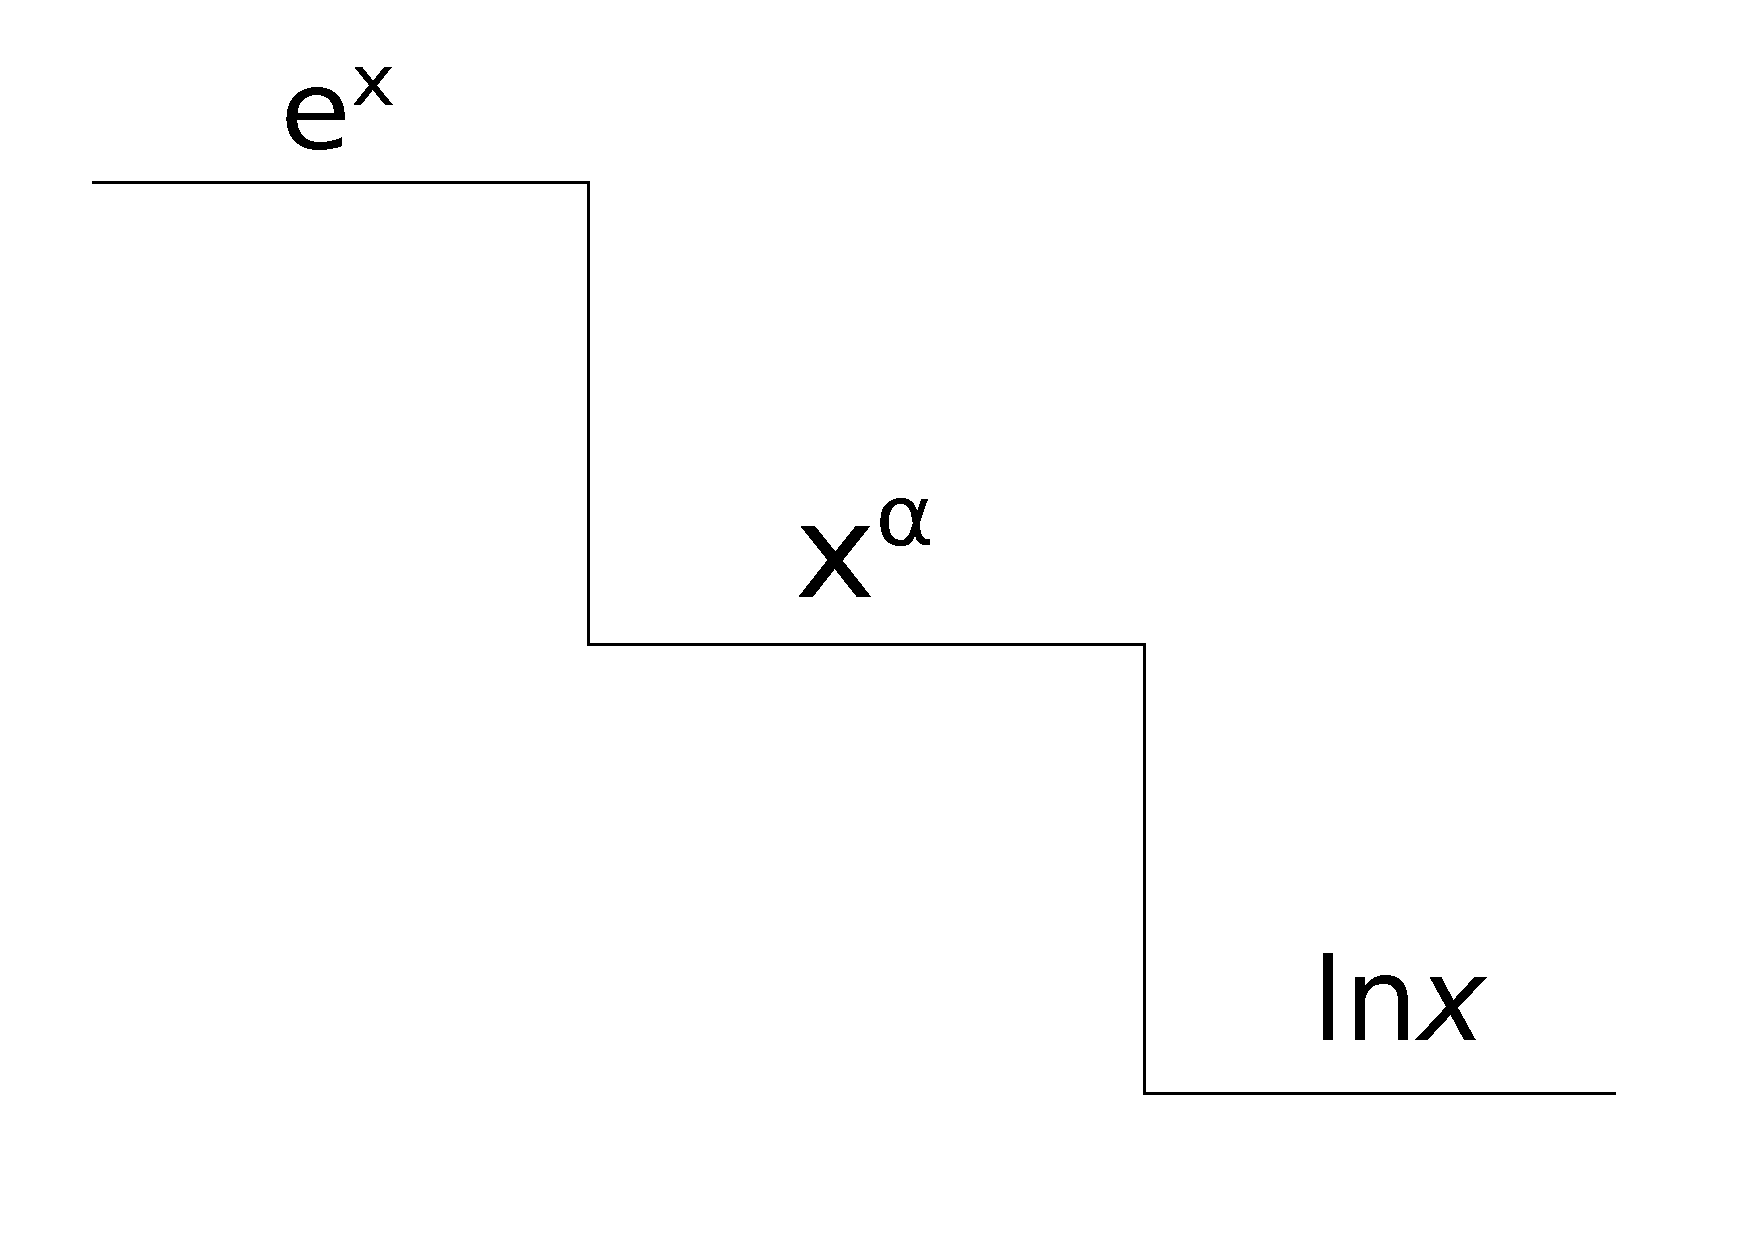
\includegraphics[height=8cm]{img/ordine di infiniti.pdf}};
	\end{tikzpicture}
	\caption{Ordine di infiniti}
\end{figure}
Siamo $f(x)$ e $g(x)$ infiniti per $x\to x_0$ (o per $x$), con $g\neq 0$. Se $\exists\alpha\in R+$ e $l\in R$, $l\neq 0$ tale che\\
$\lim_{x\to x_0}\frac{f(x)}{[g(x)]^2}=l$ (o $\lim_{x\to \infty}\frac{f(x)}{[g(x)]^\alpha}=l$)\\
Allora, per $x\to x_0$ (o per $x\to \infty$), $f(x)$ è un infinito di ordine $\alpha$ rispetto all'infinito compone $g(x)$.
\subparagraph{Esempi}
\begin{itemize}
	\item $ord(\sqrt{x})=\frac{1}{2}$ rispetto ad $x$ per $x\to +\infty$
	\item $ord(\frac{1}{\sin x})=1$ rispetto ad $\frac{1}{x}$ per $x\to 0$
	\item $ord(\frac{1}{e^x-1})=1$ rispetto ad $\frac{1}{x}$ per $x\to 0$
\end{itemize}
\subparagraph{Confronto tra infiniti}
Siamo $f(x)$ e $g(x)$ infiniti per $x\to x_0$
\begin{equation*}
	\lim_{x\to x_0}\frac{f(x)}{g(x)}=\begin{cases}
		l\neq 0&ord(f)=ord(g)\\
		\pm \infty&ord(f)>ord(g)\\
		0&ord(f)<ord(g)\\
		\text{non esiste,} & \text{f e g non confrontabile} \\ 
	\end{cases}	
\end{equation*}
Stesso risultato se $f(x)$ e $g(x)$ sono infinite per $x \to \infty$. Utilizzando il confronto tra infiniti nel calcolo dei limiti del tipo $\lim_{x\to x_0}\frac{f_1+f_2}{g_1+g_2}$, deve $f_1,f_2,g_1,g_2$ sono funzioni infinite per $x\to x_0$, si possono {\color{red}trascurare gli \underline{infiniti} di ordine minore} (analogo discorso per funzione infinito $x\to \infty$).
\subparagraph{Esempio}
$\lim_{x\to +\infty}\frac{x^2+x^3+3\sqrt{x}}{x^2(2x-1)+\sqrt{3x}}=\lim_{x\to +\infty}\frac{x^3}{2x^3}=\frac{1}{2}$.
\paragraph{Gerarchia degli infiniti}
Per $x\to +\infty$ si ha $(\log_\alpha x)^\alpha<<x^\beta<<b^x$, con $\alpha,\beta>0,a,b>1$ Non sempre è possibile calcolare l'ordine di infinito (o di infinitesimo) rispetto alla funzione campione usuale.
\subparagraph{Esempio}
\begin{equation}\label{Esempio di gerarchia degli infiniti}
	\lim_{x\to +\infty}\frac{a^x}{x^a}=+\infty, \forall \alpha>0, a>1, \lim_{x\to +\infty}\frac{(\log_a x)^\beta}{x^a}=+\infty, \forall \alpha, \beta>0, a>1	
\end{equation}
\subsubsection{Esercizio di esempio}
\begin{equation*}
	\lim_{x\to \infty} \left(\frac{e^x+x^3+\ln^4x}{e^x+x^5+\ln^6x} \right)
\end{equation*}
In questo caso al contrario degli infinitesimi, qui dobbiamo escludere i limiti di ordine più basso, ovviamente, bisogna identificarli e questo è il risultato:
\begin{equation*}
	\lim_{x\to \infty} \left(\frac{\overbrace{e^x}^\text{ordine superiore}+x^3+\ln^4x}{\overbrace{e^x}^\text{ordine superiore}+x^5+\ln^6x} \right)
\end{equation*}
una volta averli identificati escludiamo tutti gli altri, ovviamente un esponenziale sarà maggiore a tutti gli altri.
\begin{equation*}
	\lim_{x\to \infty} \frac{e^x}{e^x}=1
\end{equation*}
L'ordine di infinito di $e^x$ è superiore a $x^\alpha$ con $0<\alpha< \infty$. L'ordine di infinito di $\ln x$ è inferiore a $x^\alpha$ con $0<\alpha< \infty$
\subparagraph{Regole aritmetiche}
Siano $f(x)$ e $g(x)$ due funzioni \emph{infinite} di ordine rispettivamente $\alpha$ e $\beta$. Allora si ha
\begin{itemize}
	\item $ord(f(x)+g(x))=\max{\alpha,\beta}$
	\item $ord(f(x)*g(x))=\alpha+\beta$
	\item $ord((f(x))^\gamma)=\alpha\gamma$
\end{itemize}
\subsection{Funzioni continue}
Una funzione continua è una funzione che, intuitivamente, fa corrispondere ad elementi sufficientemente vicini del dominio elementi arbitrariamente vicini del codominio.
\paragraph{Definizione} Una funzione $f(x)$ è continua in $x_0$, se: $l_1=\lim_{x\to x^+_0}=\lim_{x\to x_0}f(x)=l_2=\lim_{x\to x_0}f(x)=f(x_0)$ ossia $\forall\in>0\exists \delta_\mathcal{E} > 0$: $|f(x)-f(x_0)|<\mathcal{E}$ $\forall_x\in I(x_0,\delta_\mathcal{E})$ $(l=f(x_0))$
\subsubsection{Teorema della permanenza del segno}
Sia f(x) definita almeno in un intorno di $x_0$ e continua in $x_0$. Se $f(x_0)>0$ allora $\exists \delta >0 : f(x) >0 \forall x\in (x_0-\delta ,x_0+\delta{})$
\subsubsection{Teorema degli zeri}
Sia $f(x)$ continua in $[a,b]$ $f(a)*f(b)<0$ allora $\exists x_0 \in (a,b): f(x_0)=0$. Se $f$ è anche strettamente monotona, lo zero è unico.
\paragraph{Teorema dell'esistenza dei valori intermedi (\textit{conseguenza del teorema degli zeri})}  
Una funzione $f(x)$ continue in $[a,b]$ assume tutti i valori compresi tra $f(a)$ ed $f(b)$.
\subsubsection{Teorema di Weierstrass (sul massimo e il minimo)}
Sia $f(x)$ continua in $[a,b]$. Allora $f(x)$ assume massimo e il minimo assoluto in $[a,b]$, cioé $\exists x_1, x_2 \in [a,b]: f(x_1)\leq f$
\subsection{Criteri di invertibilità}
Una funzione continua e strettamente monotona in $[a,b]$ è invertibile in tale intervallo. Dimostrazione.
\section{Calcolo differenziale per funzioni di una variabile}
Sia \textit{f}: $(a,b)\to R$, si definisce derivata di \textit{f} nel punto
$x_0\in (a,b)$ il numero, se $\exists$ finito:
\begin{equation*}
	f^, (x_0)=\lim_{h\to 0}\frac{f(x_0+h)-f(x_0)}{h}
\end{equation*}
\begin{equation*}
	f^\prime(x_0),y^\prime(x_0),\frac{df}{dx}|_{x_0}, \frac{dy}{dx}|_{x_0},
	Df(x_0),Dy(x_0
\end{equation*}
\subsection{Derivata di una funzione}
\paragraph{Significato geometrico della derivata in un punto e equazione della
retta tangente}
Sia $x_0\in (a,b):\text{ }x_0+h\in (a,b)$\\
\textit{Si definisce Rapporto incrementale} $\frac{\Delta f}{\Delta x}
=\frac{f(x_0+h)+f(x_0)}{h}=\tan \beta$

\begin{figure}[!ht]
	\centering
	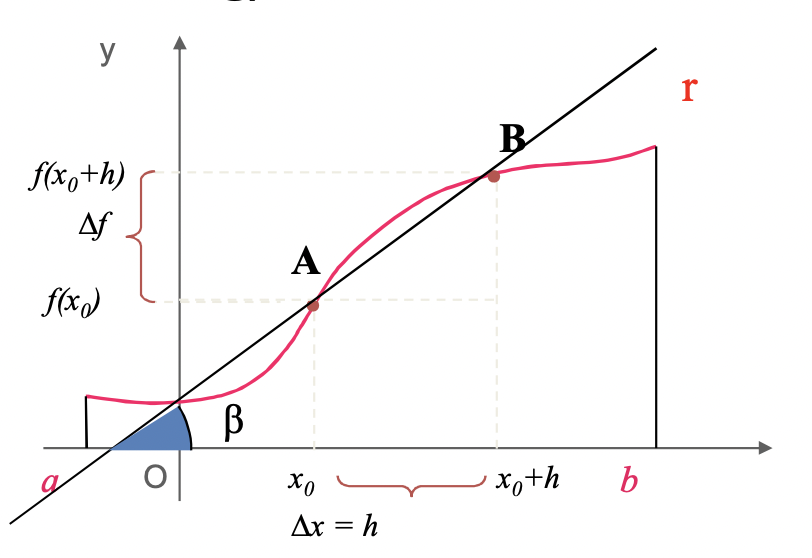
\includegraphics[height=6cm]{img/retta tangente.png}
	\caption{$\frac{\Delta f}{\Delta x}
=\frac{f(x_0+h)+f(x_0)}{h}=\tan \beta$}
\end{figure}
Sia $\beta$ l'angolo che la retta \textit{r} forma con l'asse delle x,
considerando il triangolo ABC possiamo scrivere $f(x+h)-f(x_0) = \tan\beta
[x_0+h-x_0]$ Ossia: $\tan\beta=\frac{f(x_0+h)-f(x_0)}{h}$

\begin{figure}[!ht]
	\centering
	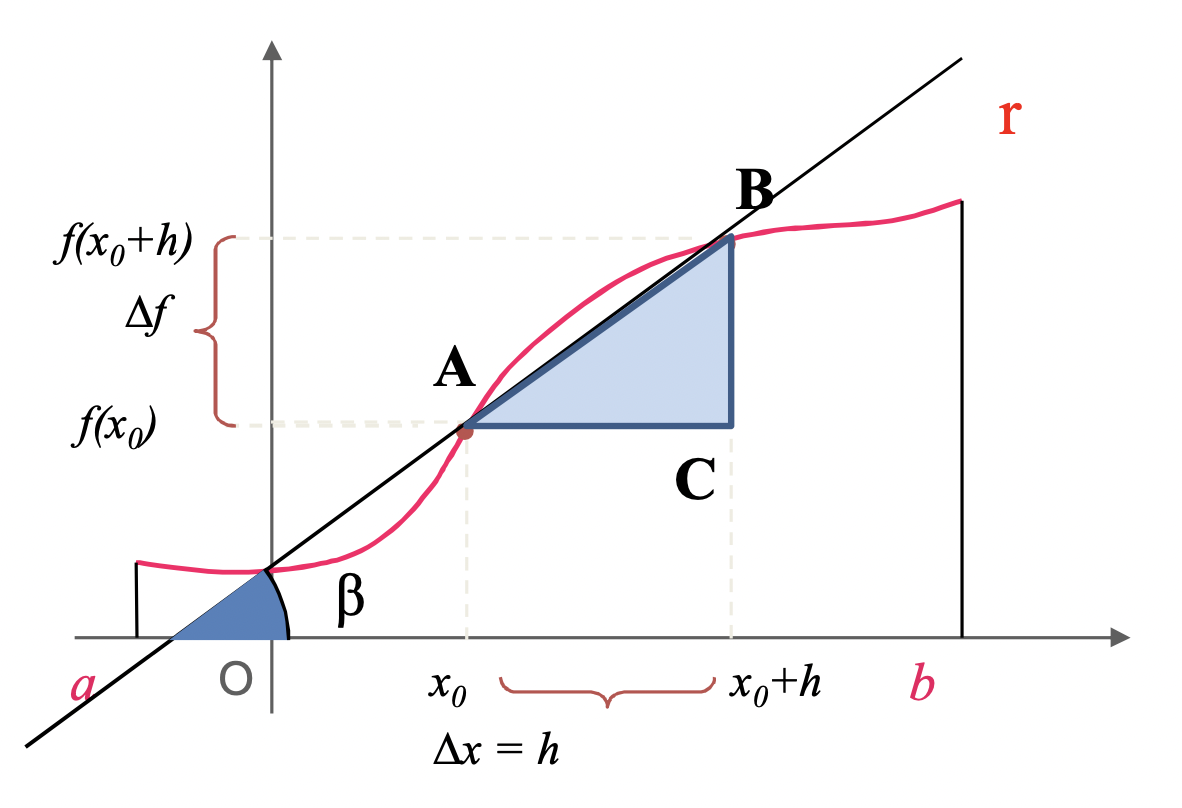
\includegraphics[height=6cm]{img/retta tangente2.png}
	\caption{$\tan\beta=\frac{f(x_0+h)-f(x_0)}{h}$}
\end{figure}
Ma $m=\frac{f(x_0+h)-f(x_0)}{h}$ È il coefficiente angolare della retta
\textit{f} passante per \textbf{AB}\\
Per cui $\tan\beta=m$

\begin{figure}[!ht]
	\centering
	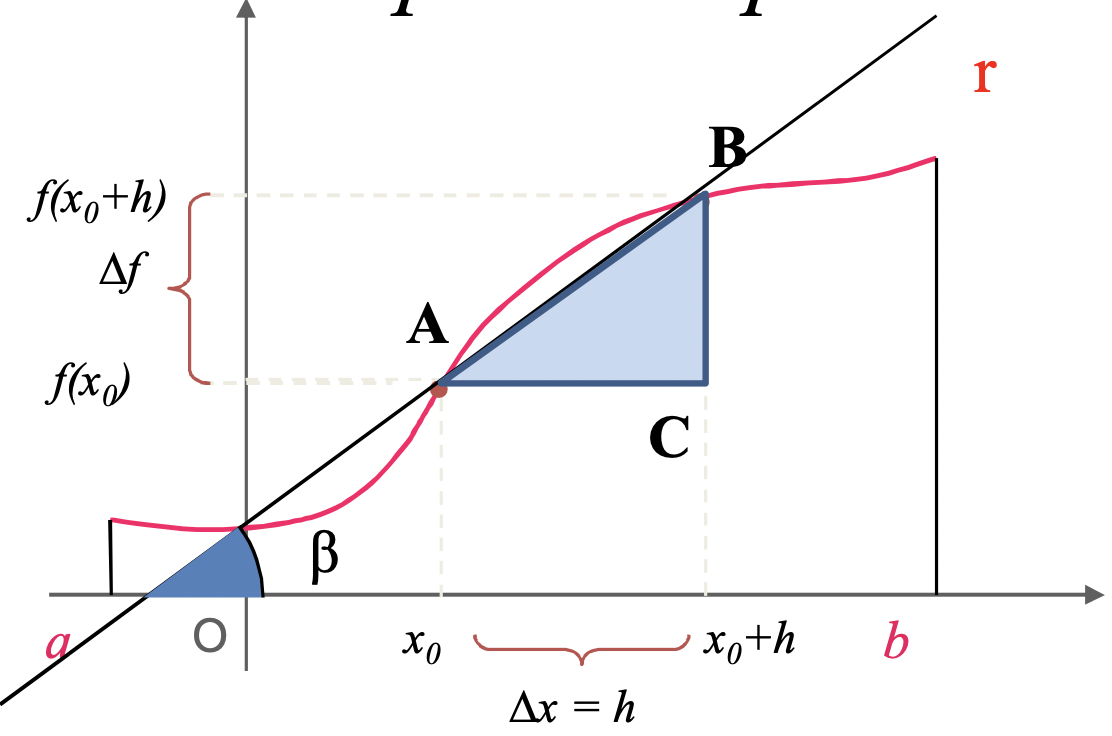
\includegraphics[height=6cm]{img/retta tangente3.png}
	\caption{$\tan\beta=m$}
\end{figure}\newpage
Ossia $\tan \beta$ è il coefficiente angolare della retta secante per AB\\
Quando $h\to 0$ in punto B si sposta sulla curva avvicinandosi ad A, la retta
\textit{r} diventa tangente alla curva in A e si ha: $\lim\limits_{h\to 0}
\frac{f(x_0+h)-f(x_0)}{h}=f^\prime(x_0)=\tan \alpha$ coefficiente angolare di t

\begin{figure}[!ht]
	\centering
	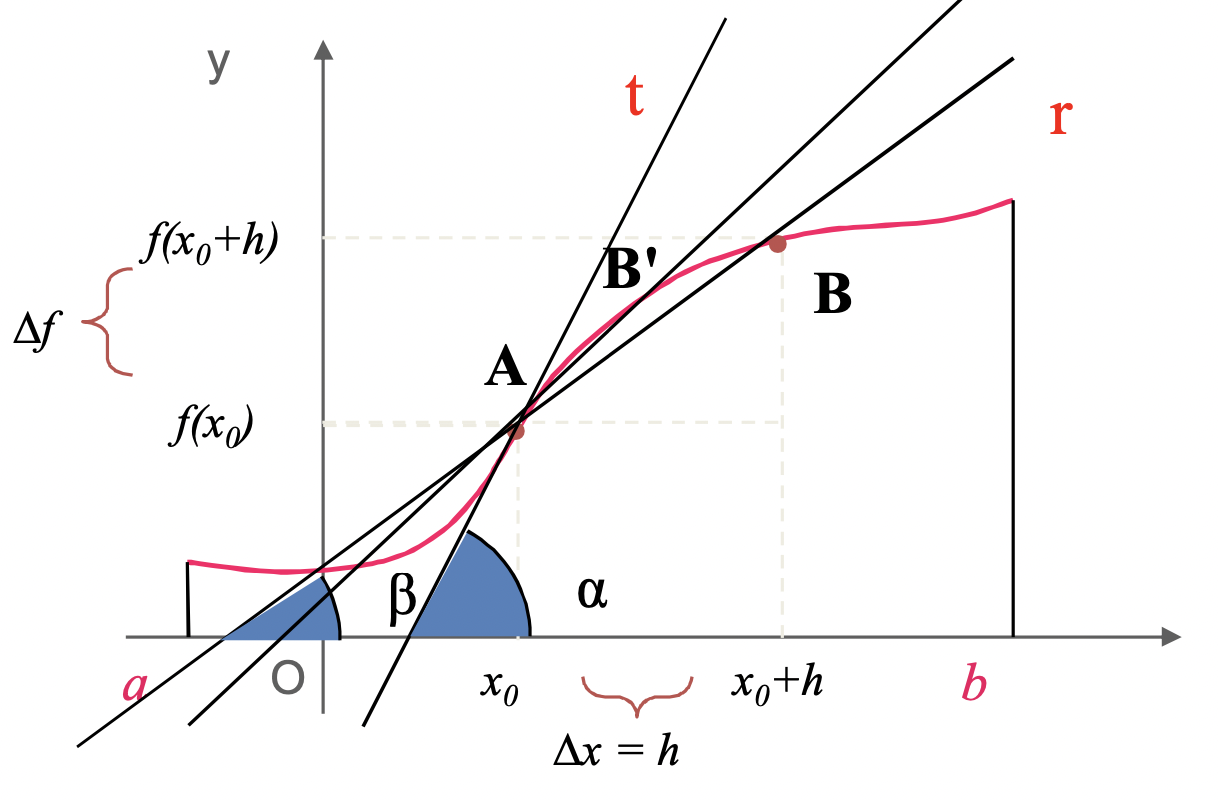
\includegraphics[height=6cm]{img/retta tangente4.png}
	\caption{$\lim\limits_{h\to 0}\frac{f(x_0+h)-f(x_0)}{h}=f^\prime(x_0)=\tan \alpha$}
\end{figure}
Equazione della retta tangente dal grafico di \textit{f(x)} nel punto di
ascissa $x_0$: $y=f^\prime(x_0)(x-x_0)+f(x_0)$ Infatti, tra tutte le rette del
fascio proprio passanti $A(x_0,f(x_0)) di eq.$ $y-f(x_0)=m(x-x_0)$ per $
m=f^\prime(x_0)$ si ottiene l'equazione di t.
% possibile grafico
Se $f^,(x)$ è definita $\forall x \in (a,b)$ allora f(x) è derivabile in (a,b)
e risulta definita la funzione $f^\prime:(a,b)\to R$ detta derivata prima di
$f(x)$\\
\textit{f(x) è derivabile in [a,b], se è derivabile $\forall x \in (a,b)$ e
ammette derivata destra in x=a (si scrive $f^,_+(a)$) e derivata sinistra in
$x=b$ (si scrive $f^\prime_-(b)$)}
\subsection{Esercizi retta tangente}
\subsubsection{Retta tangente di $f(x)=e^{\frac{1}{x}}$ in un intervallo $[a,b]$}
\begin{equation*}
	f(x)=e^{\frac{1}{x}}
\end{equation*}
\begin{equation*}
	f^\prime(x)=e^{\frac{1}{x}}*\left(-\frac{1}{x^2}\right)
\end{equation*}
\paragraph{Retta tangente nel punto A}
\begin{equation*}
	m=f^\prime(-2)=e^{-\frac{1}{2}}*\left(-\frac{1}{4}\right)=\frac{1}{4\sqrt{e}}
\end{equation*}
\fbox{
	\addtolength{\linewidth}{-2\fboxsep}%
	\addtolength{\linewidth}{-2\fboxrule}%
 	\begin{minipage}{\linewidth}
		\begin{equation*}
			y-y_A=m\left(x-x_A\right)
		\end{equation*}
	\end{minipage}
}
\begin{equation*}
	y-\frac{1}{\sqrt{e}}=\frac{1}{4\sqrt{e}}(x+2)
\end{equation*}
\begin{equation*}
	y=\frac{1}{4\sqrt{e}}+\frac{1}{2\sqrt{e}}+\frac{1}{\sqrt{e}}
\end{equation*}
\begin{equation*}
	\frac{4\sqrt{e}y}{4\sqrt{e}}=\frac{x+2+1}{4\sqrt{e}}
\end{equation*}
\begin{equation*}
	4\sqrt{x}y=x+3
\end{equation*}
\begin{equation*}
	\begin{matrix}
		-x+4\sqrt{e}y-3=0\\
		x-4\sqrt{e}y+3=0
	\end{matrix}
\end{equation*}
\paragraph{Retta tangente nel punto B}
\begin{equation*}
	m=f^\prime(-1)=e^{-1}(-1)=\frac{1}{e}
\end{equation*}
\fbox{
	\addtolength{\linewidth}{-2\fboxsep}%
	\addtolength{\linewidth}{-2\fboxrule}%
 	\begin{minipage}{\linewidth}
		\begin{equation*}
			y-y_B=m\left(x-x_B\right)
		\end{equation*}
	\end{minipage}
}
\begin{equation*}
	y-\frac{1}{e}=\frac{1}{e}\left(x-1\right)
\end{equation*}
\begin{equation*}
	y=-\frac{1}{e}=-\frac{1}{e}x-\frac{1}{e}+\frac{1}{e}
\end{equation*}
\begin{equation*}
	\boxed{
		y=-\frac{1}{e}x
	}
\end{equation*}
\subsubsection{Retta tangente di $f(x)=e^{3\ln{x}}$}
\begin{equation}
	f(x)=e^{3\ln{x}}=e^{\ln{x^3}}=x^3
\end{equation}
Determinare la retta tangente nel punto P di ascissa $x=-2$.
\paragraph{Soluzione} $f(-2)=(-2)^3$
\begin{enumerate}
	\item $P(-2;-8)$
	\item $f^\prime(x)=3x^2$
	\item $m=f^\prime(-2)=3(-2)^2=3*4=12$
	\item $y-y_B=m\left(x-x_B\right)$
	\begin{equation*}
		\begin{matrix}
			y+8=12(x+2)\\
			y=12x+24-8\\
			\boxed{y=12x+16}
		\end{matrix}
	\end{equation*}
	\begin{eqnarray*}
		f^\prime=3x^2\\
		f^{\prime\prime}=6x
	\end{eqnarray*}
\end{enumerate}
\begin{figure}[!ht]
	\centering
	\begin{tikzpicture}
		\node[] (pic) at (0,0) {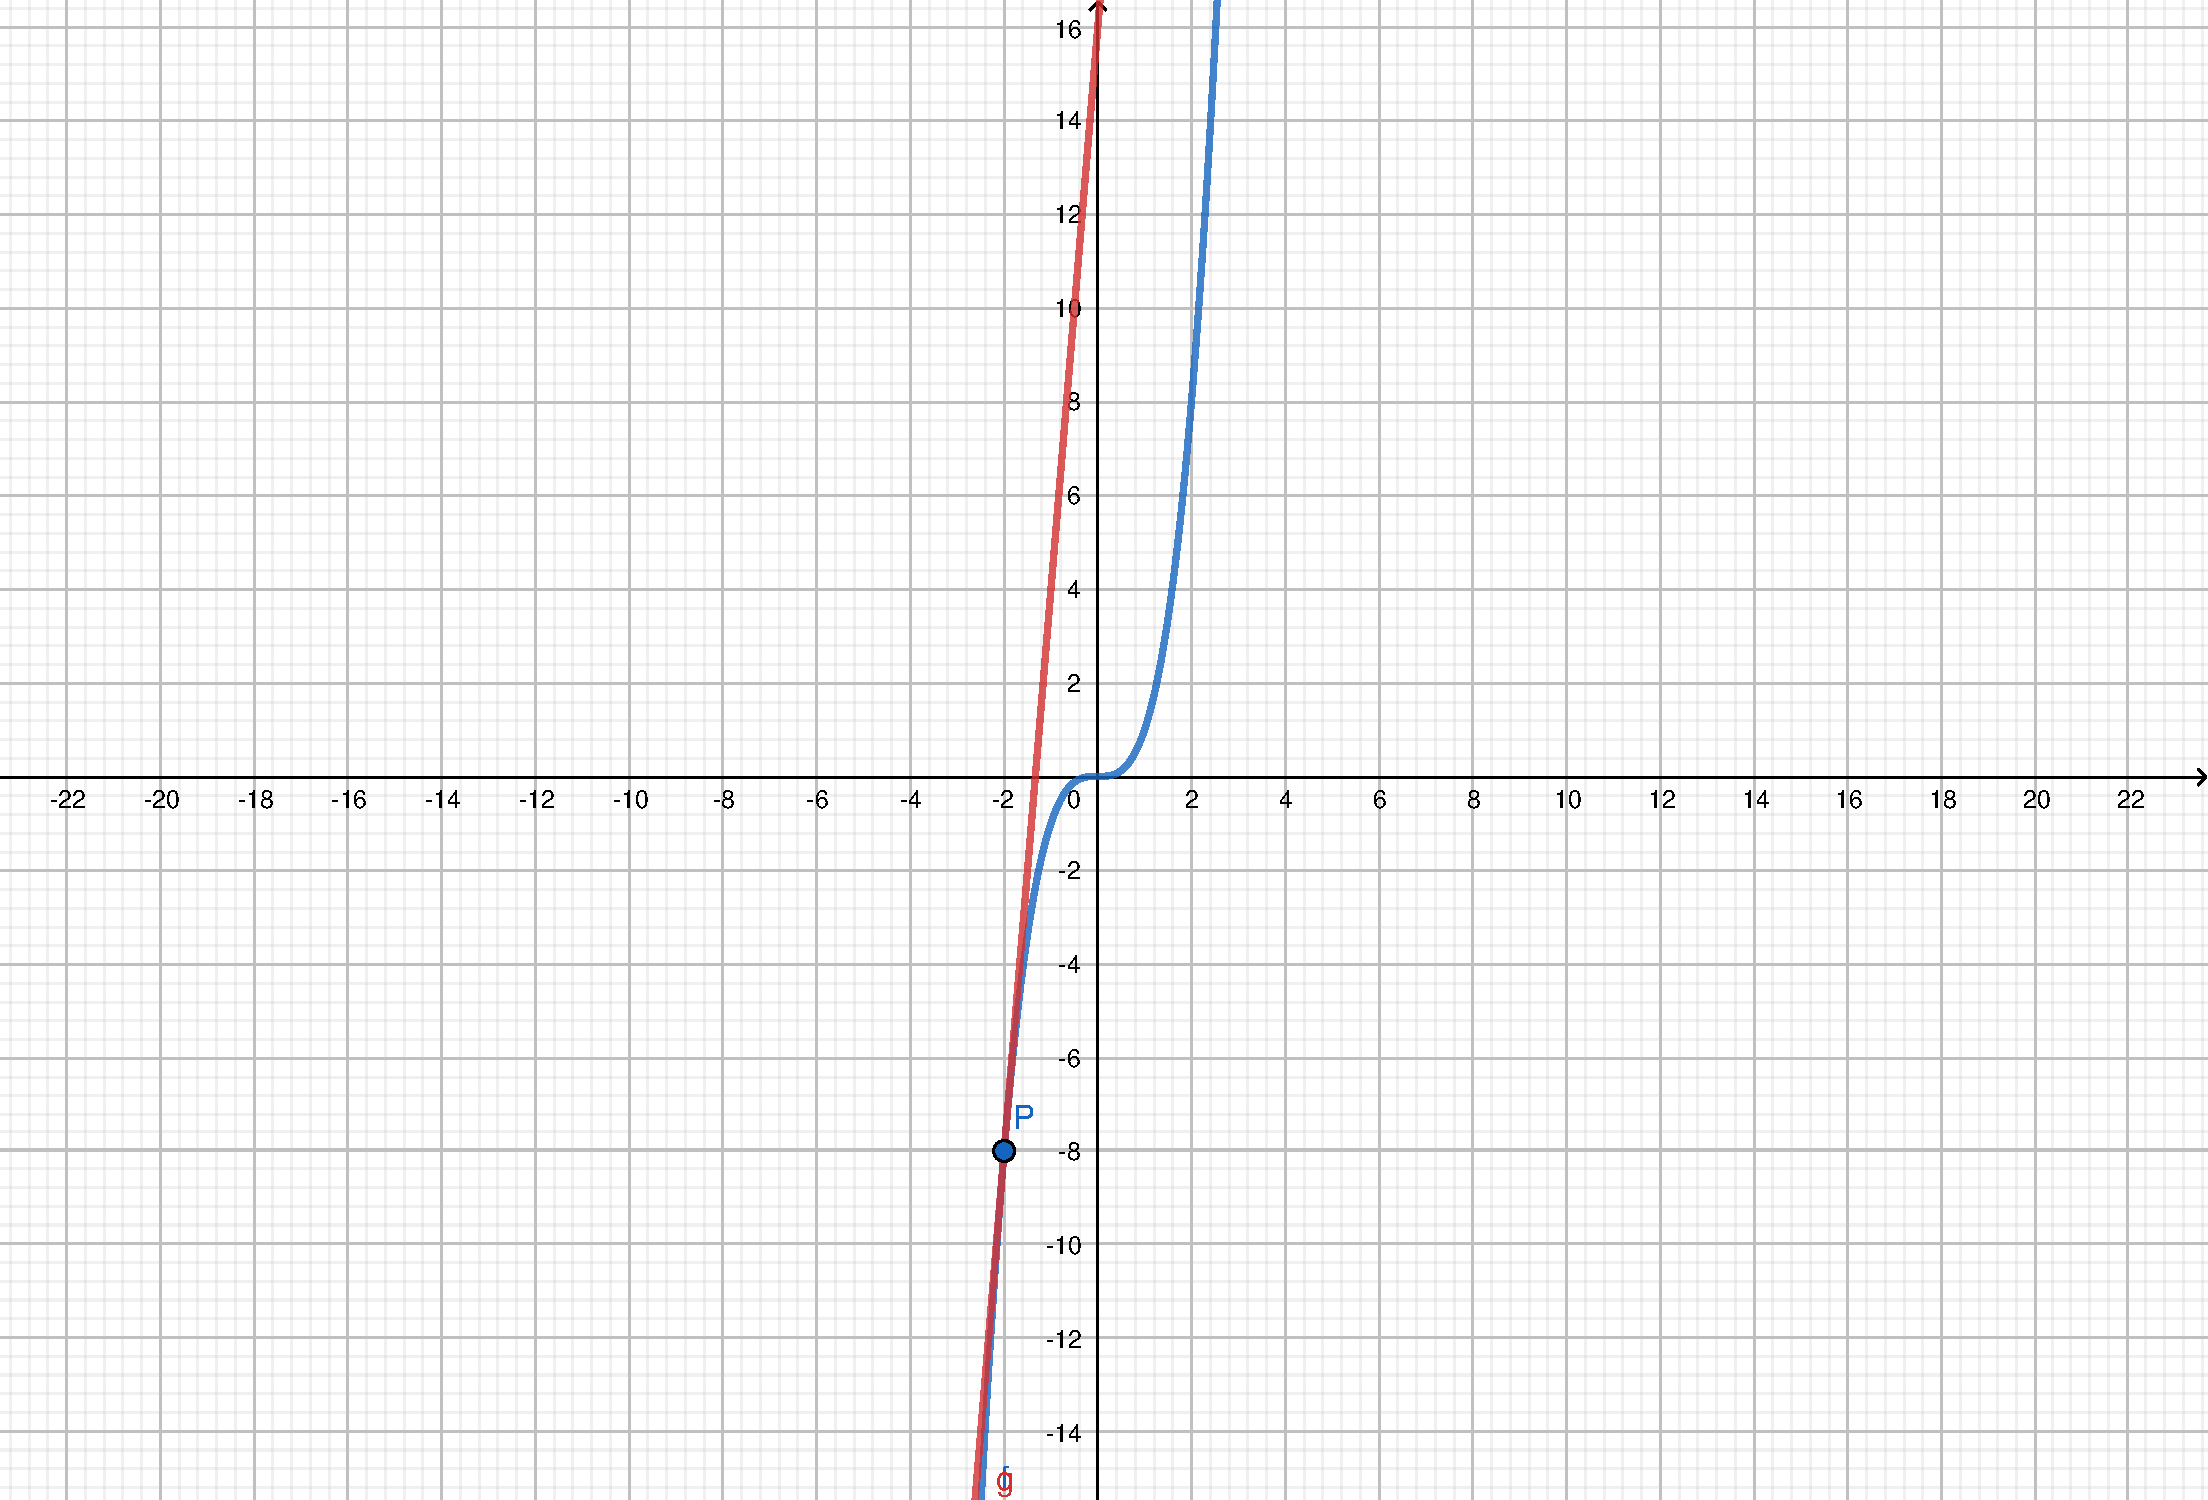
\includegraphics[height=8cm]{img/esercizio retta tangente 1.pdf}};
	\end{tikzpicture}
	\caption{Grafico di Funzione lineare $y=mx+qm, q\in R$}
\end{figure}

\subsection{Definizione}
\begin{itemize}
	\item \underline{Derivata destra} $\lim\limits_{h\to 0^+}\frac{f(x_0+h)-f(x_0)}{h}
		= f^\prime_+(x_0)$
	\item \underline{Derivata sinistra} $\lim\limits_{h\to 0^-}\frac{f(x_0+h)-f(x_0)}{h}
		= f^\prime_-(x_0)$
\end{itemize}
Se $f^,_+(x)=f^,_-(x)$ \textit{f è derivabile in x}
\subsection{Continuità e derivabilità}
\subsubsection{Teorema}\label{Teorema della continuità}
Sia $f: (a,b) \to R$. \textit{Se f è derivabile in $x_0 \in (a,b)$ allora f è
continua in $x_0,x+h\in (a,b)$: $\lim_{h\to 0} f(x_0+h)-f(x_0)=\lim_{h\to
0}\frac{f(x_0+h)-f(x_0)}{h}*h=0$}.
Da cui $\lim_{h\to 0}f(x_0+h)=f(x_0)$ che è la continuità di $f$ in $x_0$.\\
Quindi \textit{\color{red} derivabilità $\Rightarrow$ continuità} Occhio non è
vero il contrario perché non per forza una funzione continua è derivabile.
\paragraph{Esempio} $y=|x|$ è continua ma non è derivabile in $x=0$.
Infatti,
\begin{equation*}
	y=|x|=\begin{cases}
		x&x\geq 0\\
		-x&x<0
	\end{cases} \text{ e } y^\prime=\frac{|x|}{x}=\begin{cases}
		1&x> 0\\
		-1&x<0
	\end{cases}
\end{equation*}
\paragraph{Dimostrazione}
Per fare questa dimostrazione verrà utilizzato un esempio molto semplice: f(x) è continua in $x_0$ se 
\begin{equation*}
	\lim_{h\to 0} f(x+h)=f(x_0)
\end{equation*}
per dimostralo ovviamente useremo il teorema descritto in \ref{Teorema della continuità} e il risultato sarà:
\begin{equation*}
	\lim_{h\to 0}\frac{f(x_0+h)-f(x_0)}{h}=f^\prime(x_0)
\end{equation*}
\begin{equation*}
	\frac{f(x_0+h)-f(x_0)}{h}=f^\prime(x_0)+\xi (h)
\end{equation*}
con $\lim\limits_{h\to 0} \xi (h)$=0
\section{Punti di non derivabilità}
\subsection{Punto angoloso}
Se $f^\prime_+\left(x\right)\neq f^\prime_-\left(x\right)$ e almeno un $\exists$ finita $x_0$ si dice
\colorbox{yellow}{punto
angoloso}, in quanto le rette tangenti alla f(x) nel punto di ascissa $x_0$
formano un angolo.
\subsubsection{Esempio}
\begin{figure}[!ht]
	\centering
	\begin{tikzpicture}
		\node[] (pic) at (0,0) {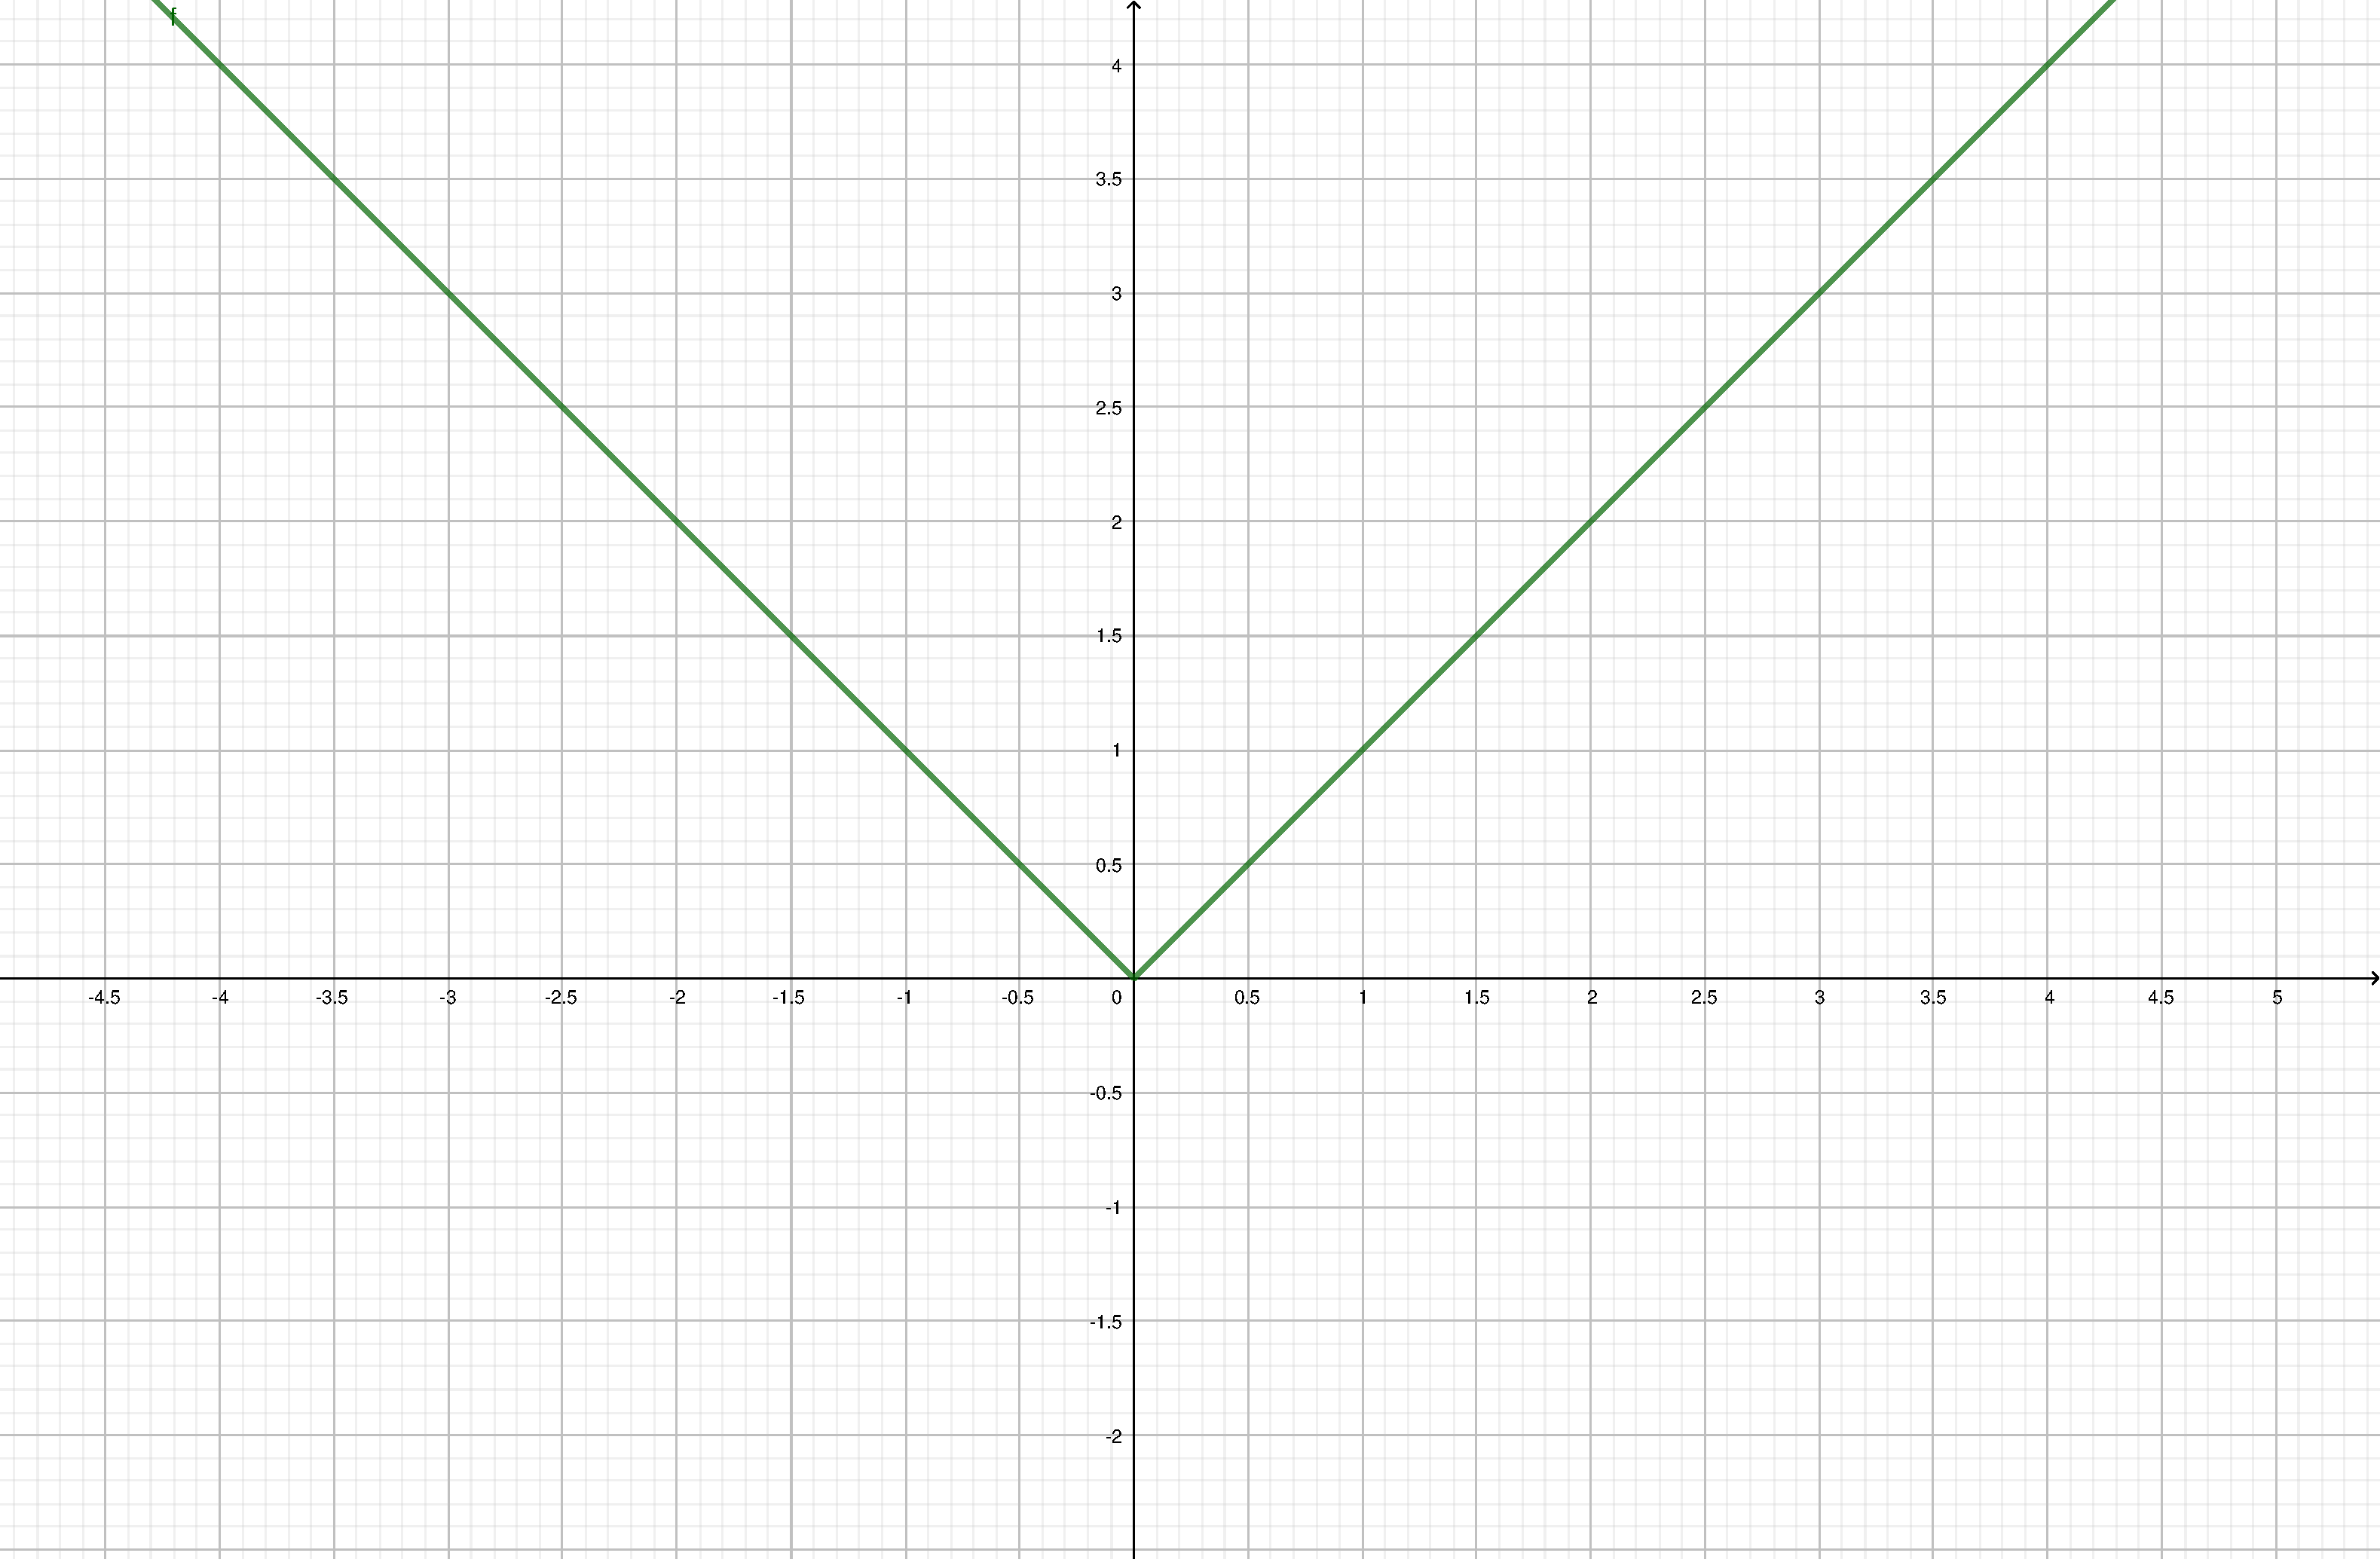
\includegraphics[height=8cm]{img/funzione valore assoluto.pdf}};
	\end{tikzpicture}
	\caption{Grafico di Funzione valore assoluto $y=|x|$ e quindi $f^,_+(0)=1\neq
	f^,_+=-1$}
\end{figure}
\subsubsection{Un altro esempio}
\begin{figure}[!ht]
	\centering
	\begin{tikzpicture}
		\node[] (pic) at (0,0) {\includegraphics[height=8cm]{img/esempio punto
		angoloso.pdf}};
	\end{tikzpicture}
	\caption{Grafico di Funzione $x=|x^2-1|$}
\end{figure}
\subsection{Punto cuspude}
Se $f^,_+(x)\neq f^,_-(x)$ sono $\infty$, $x_0$ si dece \colorbox{yellow}{punto
cuspide}; la retta tangente alla \textit{f(x)} nel punto di ascissa $x_0$ è
verticale.
\begin{figure}[!ht]
	\centering
	\begin{tikzpicture}
		\node[] (pic) at (0,0) {\includegraphics[height=8cm]{img/esempio punto
		cuspide.pdf}};
	\end{tikzpicture}
	\caption{Grafico di Funzione $f(x)=\frac{\left(x-3\right)^{\frac{2}{3}}}{2}$}
\end{figure}
\subsubsection{Punto di flesso a tangente verticale}
Se $f^,_+(x_0)=f^,_-(x_0)=\pm \infty$ sono $\infty$, $x_0$ si dice punto di
flesso a tangente verticale; la retta tangente alla $f(x)$ nel punto di ascissa
$x_0$ è verticale.
\subsection{Esempi di derivate}
\begin{multicols}{2}
	\begin{itemize}
		\item $D(x^n)=n*x^{n-1}$
		\item $D(\log_ax=\frac{1}{x}\log_a e)$
		\item $D(a^x)=a^x\ln a$
		\item $D(\sin x)=\cos x$
		\item $D(\cos x)=-\sin x$
		\item $D(k)=0$
		\item $D(\ln x)=\frac{1}{x}$
		\item $D(e^x)=e^x$
		\item $D(\tan x)=\frac{1}{\cos^2 x}=1+\tan^2x$
		\item $D(\arcsin x)=\frac{1}{\sqrt{1-x^2}}$
		\item $D(\arccos x)=-\frac{1}{\sqrt{1-x^2}}$
		\item $D(\arctan x)=\frac{1}{1+x^2}$
	\end{itemize}
\end{multicols}
\subsubsection{Qualche esercizio dimostrativo}
Utilizzando la definizione calcolare la derivata di
\begin{enumerate}
	\item $f(x)=k$\\
		$f^\prime(x)=\lim\limits_{h\to 0}\frac{f(x+h)-f(x)}{h}=\lim_{h\to 0}\frac{k-k}{h}=0$
	\item $f(x)=e^x$\\
		$f^\prime(x)=\lim\limits_{h\to 0}\frac{f(x+h)-f(x)}{h}=\lim_{h\to
		0}\frac{e^x(e^h-1)}{h}=e^x$
	\item $f(x)=\ln x$\\
		$f^\prime(x)=\lim\limits_{h\to 0}\frac{f(x+h)-f(x)}{h}=\lim_{h\to
		0}\frac{\ln(x+h)\ln x}{h}=\frac{\ln(1+\frac{h}{x})}{h}=\frac{1}{x}$
	\item $f(x)=\cos x$\\
		$f^\prime(x)=\lim\limits_{h\to 0}\frac{f(x+h)-f(x)}{h}=\lim\limits_{h\to
		0}\frac{\cos(x+h)-\cos(x)}{h}=\lim\limits_{h\to 0}\frac{\cos x*\cos h-\sin
		x*\sin h-\cos(x)}{h}=$\\$\lim\limits_{h\to 0}\frac{\cos x (\cos h -
		1)}{h}-\frac{\sin x\sin h}{h}=-\sin x$
	\item $f(x)=\sin x$\\
		$f^\prime(x)=\lim\limits_{h\to 0}\frac{f(x+h)-f(x)}{h}=\lim\limits_{h\to
		0}\frac{\sin(x+h)-\sin(x)}{h}=\frac{\sin x \cos h +\sin h \cos x-\sin
		x}{h}=\lim\limits_{h\to 0}\frac{\sin x(\cos h-1)}{h}+\lim_{h\to 0}\frac{\sin
		h\cos x}{h}=\cos x$
\end{enumerate}
\textit{Se f e g sono derivabile in x, allora sono derivabili in x anche la
somma, la differenza, il prodotto, il quoziente (con il denominatore$\neq 0$) e
si ha:}
\begin{enumerate}
	\item $(f\pm g)^\prime=f^\prime\pm g^\prime$
	\item $(f*g)^\prime=f^\prime*g+f*g^\prime$
	\item $(\frac{f}{g})^\prime=\frac{f^\prime*g-f*g^\prime}{g^2}, g\neq 0$
\end{enumerate}
\begin{itemize}
	\item \textit{Dimostriamo la 2)} $(f*g)^\prime=f^\prime*g+f*g^\prime$\\
		$(f*g)^\prime=\lim_{h\to 0}\frac{f(x+h)g(x+h)-f(x)g(x)}{h}=\lim_{h\to
0}\frac{f(x+h)g(x+h)\pm f(x)g(x+h)-f(x)g(x)}{h}=$\\
		$\lim_{h\to
0}\frac{g(x+h)[f(x+h)-f(x)]}{h}+\lim_{h\to 0}\frac{f(x)[f(x+h)-f(x)]}{h}$\\
Per ipotesi f e g sono derivabile, quindi continue in x, perciò:\\
$\lim_{h\to 0}g(x+h)=g(x),$
\begin{center}
	$(f*g)^\prime=...=f^\prime(x)*g(x)+f(x)*g^\prime(x)$
\end{center}
\item \textit{Dimostriamo la 3)}\\
	$(\frac{f}{g})^\prime=\frac{\frac{f(x+h)}{g(x+h)}-\frac{f(x)}{g(x)}}{h}=\frac{f(x+h)g(x)-f(x)g(x+h)}{g(x+h)g(x)*h}=\frac{f(x+h)g(x)-f(x)g(x+h)\pm
		f(x)g(x)}{g(x+h)g(x)*h}$\\
		$\frac{[f(x+h)-f(x)]g(x)-f(x)[g(x+h)-g(x)]}{g(x+h)g(x)*h}=\frac{\frac{[f(x+h)-f(x)]g(x)}{h}-\frac{f(x)[g(x+h)-g(x)]}{h}}{g(x+h)g(x)*h}=$\\$\frac{f^,(x)g(x)-f(x)g^,(x)}{g(x+h)g(x)*h}=\frac{f^,(x)g(x)-f(x)g^,(x)}{[g(x)]^2*h}$

\end{itemize}
\subsubsection{Esercizio}
\begin{itemize}
	\item \textit{Calcolare la derivata di $f(x)=\sin x \ln x$}\\
		$f^\prime(x)=\cos x \ln x+\frac{sin x}{x}$
	\item \textit{Scrivere l'equazione della retta tangente alla curva di eq
		$f(x)=2e^x\sqrt[3]{x}$ nel punto di ascissa x=1}\\
		$f^\prime(x)=2e^x\sqrt[3]{x}+2\frac{e^x}{3\sqrt[3]{x^2}}$
\end{itemize}
\subsection{Teorema di derivazione della funzione composta}
\textit{Sia g(x) una funzione derivabile in x, e se f(x) è una funzione
derivabile nel punto g(x), allora la funzione composta f(g(x)) è derivabile in
x, e si ha:}
\begin{center}
	$[f(g(x))]^\prime=f^\prime(g(x))*g^\prime(x)$
\end{center}
Dimostrazione. Se $h\neq 0$ si ha $\lim_{h\to
0}\frac{f(g(x+h))-f(g(x))}{h}=\lim_{h\to
0}\frac{f(g(x+h))-f(g(x))}{h}*\frac{g(x+h)-g(x)}{h}=f^\prime(g(x))*g^\prime(x)$
\textit{in quanto se $h\to 0$ allora $k\to 0$ con $k=g(x+h)-g(x)$, essendo
g(x) continua in x. Se h=0, il teorema continua a valere.}
\subsubsection{Esercizio}
\begin{enumerate}
	\item Calcolare la derivata di $f(x)=\ln(\sin x)$.\\
		$f^\prime (x)=\frac{\cos x}{\sin x}=\cot{x}$
	\item Calcolare la derivata di $f(x)=e^{\sqrt{2x^3+x}}.$\\
		$f^\prime (x)=e^{\sqrt{x^3+x}}\frac{6x^2+1}{2\sqrt{2x^3+x}}$
	\item Calcolare la derivata di $f(x)=\sin(\ln x)$\\
		$f^\prime (x)=\frac{\cos(\ln x)}{x}$
\end{enumerate}
Scrivere l'equazione della retta alla curva di equazione $f(x)=(xe^{2x}-1)^3$
nel punto di ascissa x=0, L'eq. Retta tangente a $f(x)$ in $x=x_0:
y=f^\prime(x_0)(x-x_0)+f(x_0)$\\
Per noi $x_0=0$\\
$f^\prime(x)=3(xe^{2x}-1)^2(e^{3x}+xe^{2x})\Rightarrow f^\prime (0)=3$\\
$f(0)=-1$\\
Quindi l'equazione è: $y=3x-1$
\subsection{Teorema di derivazione della funzione inversa}
\textit{Sia f(x) una funzione continua e strettamente monotona in [a,b]. Se f è
derivabile in $x_0\in(a,b)$ e se allora anche la funzione inversa di $f^{-1}$ è
derivabile nel punto $y_0=f(x_0)$, e la derivata vale:}
\begin{center}
	$[f^{-1}(y_0)]^\prime=\frac{1}{f^\prime(x_0)}$
\end{center}
Dimostrazione. Si ha
$\frac{f^{-1}(y_0+k)-f^{-1}(y_0))}{k}=\frac{h}{f(x_0+h)-f(x_0}$
% grafici
Se $k\to 0$ anche $h\to0$ in quanto $f^\prime$ è continua
\subsection{Esercizio}
Utilizzando il teorema di derivazione della funzione inversa, dimostrare che:
\begin{center}
	$D[\arcsin(y)]=\frac{1}{\sqrt{1-y^2}}$
\end{center}
$x=\arcsin(y)$ è la funzione inversa di $y=\sin(x)$ quest'ultima è invertibile
per $x\in [-\frac{\pi}{2};\frac{\pi}{2}]$. Applichiamo il teorema della
funzione inversa, $f^{-1}(y)=\frac{1}{f^\prime(x)}$\\
\begin{tabular}{|l|}
	\hline
	$[\arcsin(y)]^\prime=\frac{1}{[\sin(x)]^\prime}=\frac{1}{\cos(x)}$\\\hline
\end{tabular}\\
Ma sappiamo che: $\cos(x)=\sqrt{1-\sin^2x}$\\
\begin{tabular}{|l|}
	\hline
	$[\arcsin(y)]^\prime=\frac{1}{\sqrt{1-\sin^2x}}=\frac{1}{\sqrt{1-y^2}}$\\\hline
\end{tabular}
\subsection{Esercizio}
Calcolare la derivata della funzione $y=e^x$ vista come funzione inversa di
$f(x)=\ln x$. Per $x>0$, si ha $x=f^{-1}(y)=e^y$
$f(x)=\ln x\Rightarrow f^\prime(x)=\frac{1}{x}$ Perciò, per il teorema della
derivata della funzione inversa si ha
$(f^{-1}(y))^\prime=\frac{1}{f^\prime(x)}\Rightarrow (e^y)^\prime=x=e^y$.
Quindi $(e^x)^\prime=e^x$
\subsection{Esercizio}
Utilizzando il teorema di derivazione della funzione inversa, dimostrare che
$(\arctan x)^\prime=\frac{1}{1+x^2}$. Sia $f(x)=\tan x$, in
$x\in[-\frac{\pi}{2},\frac{\pi}{2}]$ si ha $x=f^{-1}(x)=\arctan y$\\
$f(x)=\tan x\Rightarrow f^\prime(x)=1+\tan^2x$. Perciò, per il teorema della
derivata della funzione inversa si ha
$(f^{-1}(y))^\prime=\frac{1}{f^\prime(x)}\Rightarrow (\arctan
y)^\prime=\frac{1}{1+\tan^2 x}=\frac{1}{1+y^2}$
\section{Massimo e minimo assoluto}
Sia $f:[a,b]\to R$, si dice M è \texttt{massimo assoluto} (o globale) di
\textit{f} in $[a, b]$ e $x_0\in[a, b]$ è un punto di massimo se
\begin{center}
	$f(x_0)=M\geq f(x),\forall x \in [a, b]$
\end{center}
\paragraph{in modo analogo:}
Si dice che m è un \texttt{minimo assoluto} (o globale) di
\textit{f} in $[a, b]$ e $x_1\in[a, b]$ è punto di minimo se 
\begin{center}
	$f(x_1)=M\leq f(x),\forall x \in [a, b]$
\end{center}
\section{Massimo e minimo relativo (o estremi locali)}
Sia $f:[a,b]\to R$, si dice che $x_0\in[a, b]$ è un punto di \texttt{massimo
relativo} (o locale) per $f(x)$ se $\exists I (x_0,\delta)$:
\begin{center}
	$f(x_0)\geq f(x),\forall x \in I (x_0,\delta)$
\end{center}
\paragraph{In modo analogo:}
si dice che $x_0\in[a, b]$ è un punto di \texttt{minimo relativo} (o locale)
per $f(x)$ se $\exists I (x_0,\delta)$:
\begin{center}
	$f(x_0)\leq f(x),\forall x \in I (x_0,\delta)$
\end{center}
\subsection{Punti Stazionari}
\textit{I punti in cui f(x) ha derivata nulla ($f^\prime=0$) Si dice punti
stazionari o critici.}
\section{Teorema di Fermat}
\textit{Sia $f(x)$ definita in [a,b] e derivabile in $x_0\in(a, b)$. Se $x_0$ è
un punto di estremo locale allora}
\begin{center}
	$f^\prime (x_0)=0$
\end{center}
\paragraph{Dimostrazione} Sia $x_0$ un punto di massimo relativo, cioè $\exists
I (x_0,\delta)$: $f(x_0)\leq f(x_0+h), \forall h: |h|<\delta$ si ha:
$\frac{f(x_0+h)+f(x_0)}{h}\begin{cases}
	\leq 0 & \text{ se } 0<h<\delta\\
	\geq 0 & \text{ se } -\delta<h<0 
\end{cases}$ e 
\begin{itemize}
	\item $\lim_{h\to 0^+}\frac{f(x_0+h)-f(x_0)}{h}=f^\prime_+\leq 0$
	\item $\lim_{h\to 0^-}\frac{f(x_0+h)-f(x_0)}{h}=f^\prime_-\geq 0$
\end{itemize}
Ma essendo $f(x)$ derivabile in $x_0$:
\begin{center}
	$f^\prime_+(x_0)=f^\prime_-(x_0)\Rightarrow f^\prime=0$
\end{center}
Se $x_0=a$ allora $0<h<\delta$ e se $x_0$ è un punto di \texttt{massimo 
relativo} si ha $\lim_{h\to 0^+}\frac{f(a+h)-f(x)}{h}=f^\prime(a)\leq 0$.
Mentre, se parliamo del \texttt{minimo relativo} in $x_0=a$: 
$\lim_{h\to 0^-}\frac{f(a+h)-f(x)}{h}=f^\prime(a)\leq 0$ In modo analogo: se
$x_0=b$ è punto di \texttt{massimo relativo} (con $-\delta<h<0$) allora
$f^\prime(b)\geq 0$, se invece $x_0=b$ è un punto di \texttt{minimo relativo},
allora $f^\prime(b)\leq 0$
\section{Teorema di Rolle}
Sia $f:[a,b]\to R$.
\begin{enumerate}
	\item \textit{f è continua in $[a,b]$},
	\item \textit{f è derivabile in $(a,b)_{f(a)=f(b)}$}
	\item $f(a)=f(b)$
\end{enumerate}
Allora $\exists x_0 \in (a,b):f^\prime(x_0)=0$ Per il Teorema di Rolle esistono
almeno un punto a tangente orizzontale.
\subsection{Dimostrazione}
Per il Teorema di Weiestrass, $f$ ha massimo e minimo assoluti in $[a,b]$
($x_1,x_2\in[a,b]$):
\begin{center}
	$f(x_1)\leq f(x)\leq f(x_2).$
\end{center}
\textit{Se uno dei due è interno ad $[a,b]$, per esempio $x_1$ allora per il
Teorema di Fermat $f^\prime(x_1)=0$. Se invece nessuno dei due è interno ad
$[a,b]$ per esempio $x_1=a, \text{ } x_2=b$. Dall'ipotesi $f(a)=f(b)$ si ottiene
minimo=massimo, cioè $f(x)$ è costante $\forall x \in[a,b]$ e quindi
$f^\prime(x)=0\text{ } \forall x \in [a,b]$}.
\subsection{Esercizio dimostrativo}
\subsubsection{Testo}
Dire se la funzione $f(x)=e^{x^2-1}$ soddisfa il teorema di Rolle
nell'intervallo $[-1,1]$ e in caso affermativo calcolare il punto (o i punto
del Teorema.)
\subsubsection{Soluzione}
Sono verificate tutte le ipotesi del teorema di Rolle, infatti:
\begin{enumerate}
	\item $f(x)=e^{x^2-1}$ è continua in tutte R e quindi anche in $[-1,1]$
	\item f(x) è derivabile in tutto R, quindi anche in (-1,1),
	\item $f(-1)=f(1)$
\end{enumerate}
Allora $\forall x_0 \in (-1,1):f^\prime(x_0)=0$\\
$x_0$ Si ricava facendo il calcolo: $f^\prime (x_0)=0$, cioè
$2xe^{x^2-1}=0\Rightarrow x_0=0$
\subsection{Esercizio dimostrativo}
\subsubsection{Testo}
Dire se la funzione $f(x)=\ln|x|$ soddisfa il teorema di Rolle nell'intervallo
[-e,e].
\subsubsection{Soluzione}
Il teorema di Rolle non è applicabile perché $f(x)=\ln|x|$ non è definita in
$x=0$, quindi non è né continua né definita in $x=0$ e perciò non soddisfa
tutte le ipotesi del teorema.
\section{Teorema di Lagrange ({\em o del valor medio})}
\begin{figure}[!ht]
	\centering
	\begin{tikzpicture}
		\node[] (pic) at (0,0) {\includegraphics[height=6cm]{img/grafico
		dimostrativo di lagrange.pdf}};
	\end{tikzpicture}
	\caption{Grafico dimostrativo del teorema di Lagrange}
\end{figure}

Sia $f:[a,b]\to R$. Per applicare il teorema devono essere rispettati i
seguenti punti:
\begin{enumerate}
	\item {\em La funzione deve essere continua in $\left[a,b\right]$;}
	\item {\em La funzione deve essere derivabile in $\left(a,b\right)$;}
	\item {\em La retta C deve tangere la funzione almeno una volta.}
\end{enumerate}
Allora $\forall x_0\in(a,b):f^\prime (x_0)=\frac{f(b)-f(a)}{b-a}$\\
\textit{Per il Teorema di Lagrange $\exists$ almeno un punto ($x_0,f(x_0)$) sul
grafico di f(x) in cui la retta tangente \textbf{t} è parallela alla retta
\textbf{r} secante la curva in $(a,f(a))$ e $b,f(b)$}.

\subsection{Esempio}
$f(x)=x^2 \text{ in } [a,b]$, per il Teorema di Lagrange $\forall x_0 \in
[a,b]$:
\begin{center}
	$\frac{b^2-a^2}{b-a}=2x_0\Rightarrow x_0=\frac{b+a}{2}$ Media aritmetica di
	a e b
\end{center}
\subsection{Esercizio dimostrativo}
\subsubsection{Testo}
\textit{Dire se è applicabile in Teorema di Lagrange alla funzione
$f(x)=\arcsin x$ nell'intervallo $[-1,1]$ e in caso affermativo calcolare i
punti teorema.}
\subsubsection{Soluzione}
La funzione data soddisfa tutte le ipotesi del teorema di Lagrange, infatti:
\begin{enumerate}
	\item $f$ è continua in [-1,1] (è il suo campo di esistenza),
	\item $f$ è derivabile in (-1,1)\\
		Allora $\forall x_0\in (-1.1):f^\prime
		(x_0)=\frac{f(1)-f(-1)}{2}\Rightarrow
		\frac{1}{\sqrt{1-x^2_0}}=\frac{\pi}{2}\Rightarrow
		x_0=\pm\frac{\sqrt{\pi^2-4}}{\pi}$
\end{enumerate}
\subsection{Esercizio dimostrativo}
\subsubsection{Testo}
Determinare un intervallo in cui è applicabile il Teorema di Lagrange alla
funzione $f(x)=|x-\frac{1}{x}|$.
\subsubsection{Soluzione}
\begin{enumerate}
	\item La funzione data è contenuta nel suo campo di esistenza cioè
		nell'insieme: $A=\{x \in R: x\neg 0\}$
	\item f è derivabile nell'insieme $B=\{x\in R: x\neq 0,\pm 1\}$ con
		derivata: $f^\prime(x)=|\frac{x^2-1}{x}|\frac{x^2+1}{x(x^2-1)}$
\end{enumerate}
Perciò un intervallo in cui $f$ soddisfa il teorema di Lagrange, è un qualunque
intervallo $[a,b]$ che contiene $x=0$ e tale che punti $x=-1$ non siano interni
ad esso (potrebbero stare agli estremi)\\
Per esempio: $[1,2]$ (f è continua in [1,2] e derivabile in (1,2), da notare
che è derivabile anche in $x=2$ ma non serve\dots) oppure $[-4,-3]$. etc\dots


\begin{enumerate}
	\item Criterio di monotonia\\
		Sia $f(x):[a,b]\to R$, continue in $[a,b]$, è derivabile in $(a,b)$.
		Allora:
		\begin{itemize}
			\item f è crescente in $[a,b]\Leftrightarrow f^\prime(x)\geq 0
				\forall x \in [a,b]$;
			\item f è crescente in $[a,b]\Leftrightarrow f^\prime(x)\leq 0
				\forall x \in [a,b]$.
		\end{itemize}
		\paragraph{Dimostrazione}
		Sia $f^\prime (x)\geq 0 \text{ e siano } x_1,x_2\in[a,b]\text{ con }
		x_2>x_1$.\\
		Per il Teorema di Lagrange $\forall x_0\in (x_1,x_2)$:	
			\begin{center}
				$f(x_2)-f(x_1)=f^\prime(x_0)(x_2-x_1)$
			\end{center}
			ma $f^\prime(x_0)\geq 0$ e $x_2-x_1>0 \Rightarrow f(x_2)\geq f(x_1)$
		\paragraph{Viceversa} Sia $f(x)$ crescente in $[a,b]$.\\
		Allora $\forall x, x+h\in (a,b)$, si ha $\frac{f(x+h)-f(x)}{h}\geq 0$\\
		Facendo il limite per $h\to 0$ si ha
		\begin{center}
			$f^\prime(x)\geq 0$
		\end{center}
		Analoga dimostrazione per
		\begin{equation}
			\text{f è decrescente in} [a,b]\Leftrightarrow f^\prime\leq 0 \forall
			x\in [a,b]
		\end{equation}
		Analoga dimostrazione per $f$ è decrescente in $[a,b]\Leftrightarrow
		f^\prime(x)\leq 0 \forall x \in [a,b]$\\
		Si ha inoltre
		\begin{itemize}
			\item $f^\prime (x)>0\Rightarrow$ strettamente crescente
			\item $f^\prime (x)<0\Rightarrow$ strettamente decrescente
		\end{itemize}
	\item Sia $f(x):[a,b]\to R$, derivabile in (a,b).
		\begin{equation}
			\text{f è costante} \Leftrightarrow f^\prime (x)=0 \forall x\in(a,b)
		\end{equation}		
	\item Sia $x_0\in (a,b)$ e $f^\prime (x_0)=0$\\
		\textit{Se esiste un intorno destro (sinistro), in cui $f^\prime (x)>0$
		e un intorno sinistro (destro) in cui $f^\prime (x)<0$, allora $x_0$ è
		un punto di minimo (massimo) relativo}.
\end{enumerate}
\section{Teorema di Cauchy}
Siamo $f,g:[a,b]\to R$:
\begin{enumerate}
	\item \textit{f e g sono continue in $[a,b]$}
	\item \textit{f e g sono derivabili in $(a,b)$}.
\end{enumerate}
Allora se $g^\prime (x) \neq 0, \forall x \in (a,b), \exists x_0\in(a,b)$:
$\frac{f^\prime (x_0)}{g^\prime (x_0)}=\frac{f(b)-f(a)}{g(b)-g(a)}$
\subsection{Dimostrazione}
Si consideri la funzione ausiliaria
\begin{center}
	$\upvarphi(x)=f(x)-[f(a)+\frac{f(b)-f(a)}{g(b)-g(a)}-(g(b)-g(a))]$
\end{center}
Essendo $g^\prime\neq 0, \forall x \in (a,b)$, allora $g(b)\neq g(a)$. Inoltre
\begin{enumerate}
	\item $\upvarphi(x)$ è continua in $[a,b]$;
	\item $\upvarphi(x)$ è derivabile in $(a,b)$;
	\item $\upvarphi(a)=\upvarphi(b)$
\end{enumerate}
\begin{center}
	$\Rightarrow \exists x_0 \in (a,b):\upvarphi^\prime(x_0)=0$
\end{center}
Cioè
\begin{center}
	$\frac{f^\prime (x_0)}{g^\prime(x_0)}=\frac{f(b)-f(a)}{g(b)-g(a)}$
\end{center}
\section{Teorema di de l'Hopital\label{del'hop}}
$\lim_{x\to x_0}f(x)=\lim_{x\to x_0}g(x)=0$ oppure $\lim_{x\to
x_0}f(x)=\lim_{x\to x_0}f(x)=\infty$\\
Se esiste il limite $\lim_{x\to x_0}\frac{f^\prime(x)}{g^\prime(x)}=l$ finito e
limitato. Allora $\lim_{x\to x_0}\frac{f(x)}{g(x)}=\lim_{x\to
x_0}\frac{f^\prime(x)}{g^\prime(x)}$\\
\texttt{Il teorema è valido anche per $x\to x_0^+$ o $x\to x_0^-$ e per $x\to
\pm\infty$ (f e g derivabili in intervalli illimitati)}
\section{Funzioni convesse e concave}
\subsection{Definizione di funziona convessa}
Sia $f(x):[a,b]\to R$, si chiama epigrafico (\textit{o sopragrafico}) di $f$
l'insieme
\begin{center}
	$epif:=\{(x,y)\in R^2:x\in[a,b]\text{ e }y\leq f(x)\}$
\end{center}
\textit{f è convessa in $[a,b]$ se il suo epigrafico è un insieme convesso}
\paragraph{Analogamenente:} \textit{f è concava in $[a,b]$ se il suo epigrafico
è un insieme concavo}\\
Sia $f(x)$ derivabile in $[a,b]$, \textit{f è convesse in
$[a,b]\Leftrightarrow f(x)\geq f(x_0)+f^\prime(x_0)(x-x_0), \forall
x,x_0\in[a,b]$}
\begin{center}
	Cioè $\forall x_0$ il grafico di $f$ sta al di sopra della retta tangente
	ad $f(x)$ in $(x_0,f(x_0))$
\end{center}
\subsection{Definizione di funziona concave}
Sia $f(x)$ derivabile in $[a,b]$, \textit{f è concava in
$[a,b]\Leftrightarrow f(x)\leq f(x_0)+f^\prime(x_0)(x-x_0), \forall
x,x_0\in[a,b]$}
\begin{center}
	Cioè $\forall x_0$ il grafico di $f$ sta al di sopra della retta tangente
	ad $f(x)$ in $(x_0,f(x_0))$
\end{center}
\subsection{Derivata seconda}
La derivata seconda di una funzione $f(x)$ rappresenta la velocità di
variazione della pendenza del grafico di $f(x)$.
\begin{center}
	$f^{\prime\prime}(0)=\frac{1}{R}$ \textit{Curvatura del grafico di $f(x)$
	in x=0}
\end{center}
\subsection{Criterio di convessità}
Sia $f:[a,b]\to R$,
\begin{enumerate}
	\item Se f è derivabile in $(a,b)$ allora
		\begin{center}
			f è convessa (concava) $\Rightarrow$ $f^\prime(x)$ è crescente
			(decrescente)
		\end{center}
	\item Se f è derivabile due volte in $(a,b)$ allora
		\begin{center}
			f è convessa (concava) $\Rightarrow f^{\prime\prime}(x)\leq
			0(f^{\prime\prime}(x)\geq 0), \forall x \in (a,b)$
		\end{center}
\end{enumerate}
Utilizzando il segno di $f^{\prime\prime}(x)$ si può stabilire se $x_0$ è un
punto di massimo i un punto di minimo relativo per $f(x)$.\\
Sia $f(x)$ derivabile due volte con derivata continua in un intorno di
$x_0\in(a,b)$:
\begin{itemize}
	\item se $f^{\prime}(x_0)=0, f^{\prime\prime}(x)>0\Rightarrow x_0$ è punto di minimo
relativo;
\item se $f^{\prime}(x_0)=0, f^{\prime\prime}(x)<0\Rightarrow x_0$ è punto di massimo
relativo.
\end{itemize}
Infatti, supponiamo che $f^{\prime}(x_0)=0, f^{\prime\prime}(x)>0$ con
$f^{\prime\prime}$ continua. Per il Teorema della permanenza del segno:
$f^{\prime\prime}(x)>0$ in $I(x_0,\delta)\Rightarrow$ è convessa in I:
\begin{center}
	$f(x)\geq f(x_0)+f^\prime(x_0)(x-x_0)$.
\end{center}
Ma $f^\prime (x_0), \Rightarrow f(x)\Rightarrow f(x) \geq f(x_0), \forall x,
x_0\in (x_0-\delta, x_0+\delta)$ cioè $x_0$ è di minimo relativo per f.
\subsection{Criterio per i punti di massimo e di minimo relativo}
\textit{Sia $f:(a,b)\to R$, derivabile n volte in $x_0\in (a,b), n\geq 2$, tale
che in $x_0$ tutte le derivate tranne l'n-esime siano nulle. Allora:}
\begin{center}
	se n pari è $\begin{cases}
		f^{(n)}(x_0)>0 & x_0\text{ è di minimo relativo}\\
		f^{(n)}(x_0)<0 & x_0\text{ è di massimo relativo}
	\end{cases}$
\end{center}
\textit{Se n è dispari $x_0$ non è punto di estremo (\underline{si dice flesso a tangente
orizzontale})}.
\subsubsection{Definizione}
Sia $f:(a,b)\to R$ e $x_0\in (a,b)$ un punto di derivabilità per $f(x)$ oppure
$f^\prime(x_0)=\pm\infty$. \textit{$x_0$ si dice di flesso se esiste un intorno
destro di $x_0$ in cui $f$ è convessa (concava) ed un intorno sinistro in cui
$f$ è concava (convessa).}\\
Se $x_0$ è di flesso per f, ed esiste $f^{\prime\prime} (x_0),\text{ allora }
f^{\prime\prime}(x_0)=0$

\section{Punti per lo svolgimento dello studio di funzione}
Per svolgere correttamente lo studio di funzione, bisogna suddividere il tutto
in punti per svolgere correttamente lo studio in modo ordinato ed efficiente.
Se effettivamente.
\begin{enumerate}
	\item Determinazione del Campo di esistenza;
	\item Determinazione del tipo di funzione;
	\item Intersezione con gli assi;
	\item Valori agli estremi del campo di esistenza;
	\item Positività e negatività;
	\item Determinazione degli asintoti;
	\item Determinazione della derivata prima;
	\item Crescenza e decrescenza;
	\item Determinazione dei Massimi e minimi;
	\item Determinazione della derivata seconda;
	\item Determinazione della concavità, convessità e flessi;
	\item Determinazione di eventuali ulteriori punti appartenenti alla
		funzione;
	\item Grafico della funzione;
	\item Qualche esempio di studio completo di funzione.
\end{enumerate}
\subsection{Studio del grafico di f(x), Asintoti}
Se esiste una retta di equazione $y=mx+q$:
\begin{equation*}
	\lim_{x\to\infty}\{f(x)- (mx+q)\}=0
\end{equation*}
Allora $y=mx+q$ si definisce \underline{\color{red}asintoto obliquo} per f(x).
Si ha
\begin{equation*}
	m=\lim_{x\to \infty}\frac{f(x)}{x}; q=\lim_{x\to \infty} f(x)-mx
\end{equation*}

Se $\lim_{x\to \infty}f(x)=l, y=l$ si chiama asintoto orizzontale.
Se l'asintoto orizzontale non c'è (il limite sopra è infinito) allora potrebbe
esserci quello obliquo. Se $\lim_{x\to x_0}f(x)=\infty, x=x_0$ si chiama
asintoto verticale con $x_0$ punto di accumulazione per f.
\section{Approssimazione di funzioni con polinomi}
\subsection{Polinomio di Taylor}
Data una funzione $f$ derivabile $n$ volte in $x_0$, esiste uno e un solo
polinomio
\begin{equation}
	T_n(x_0)=f(x_0),T^\prime_n(x_0)=f^\prime(x_0),\dots, T^{(n)}(x_0)=f^{(n)}(x_0).
\end{equation}
Tale polinomio si chiama polinomio di Taylor ed è
\begin{equation}
	T_n(x)=f(x_0)+f^\prime(x_0)(x-x_0)+\frac{f^{\prime\prime}(x_0)}{2}(x-x_0)^2+\dots
	+ \frac{f^{\prime\prime}(x_0)}{n!}(x-x_0)^n
\end{equation}

Polinomio di centro $x_0$ e grado n
\begin{equation}
	T_n(x)=\sideset{}{^n}\sum_{k=0}\frac{f^{(b)}(x_0)(x-x_0)^k}{k!}(x-x_0)^k
\end{equation}

Se $x_0=0T_n(x)$ è detto polinomio di Mac Laurin di grado n. $R_n(x)=$ errore
che si commette quando si approssima $f(x)$ con $T_n(x)$:\\
Si ha: $R_n(x)=f(x)-T_n(x)$
\begin{itemize}
	\item $R_n(x)=o((x-x_0)^n)$ per $x\to x_0$, \underline{Formula di Peano}
		\begin{equation*}
			\text{cioè }\lim_{x\to x_0}\frac{R_n(x)}{(x-x_0)^n}=0
		\end{equation*}
	\item \textit{Se f è derivabile $n+1$ volte in $(a,b)$ ecluso al più
		$x_0$,}\\
		$\forall x\in(a,b), \exists c$ compreso tra $x$ e $x_0$:\\
		$R_n(x)=\frac{f^{(n+1)}(c)}{(n+1)!}(x-x_0)^{n+1}$ Formula di Lagrange
\end{itemize}
Esempio.
\begin{equation*}
	y=\sin x \text{ in } x=0,\text{ }T_{2n+1}(x)=\sideset{}{^n}\sum_{k=0}(-1)^k \frac{x^{2k+1}}{(2k+1)!} \text{ solo potenze dispari}
\end{equation*}
\begin{itemize}
	\item $T_1(x)=x$
	\item $T_3(x)=x-\frac{x^3}{3!}$
	\item $T_5(x)=x\frac{x^3}{3!}+\frac{x^5}{5!}$
\end{itemize}
\begin{equation*}
	\text{Analogamente in } x=0,\text{ si ottiene}
\end{equation*}
\begin{equation*}
	\ln(1+x)=x-\frac{x^2}{2}+\frac{x^3}{3}-\dots (-1)^{n+1}\frac{x^{n}}{n}+R_n(x)
\end{equation*}
\begin{equation*}
	e^x=1+x+\frac{x^2}{2}+\frac{x^3}{3!}-\dots\frac{x^{n}}{n!}+R_n(x)
\end{equation*}
\begin{equation*}
	\arctan x = x-\frac{x^3}{3}+\frac{x^5}{5}-\dots\frac{x^{2n+1}}{2n+1}+R_{2n+1}(x)
\end{equation*}

\section{Calcolo integrale per funzioni di una variabile}
\subsection{Integrale definito}
Sia $f:[a,b]\to R$, \text{limitata}
Costruiamo la somma di Cauchy-Riemann
\begin{equation*}
	S_n= \sideset{}{^n}\sum_{j=1}f(\xi_j)*(x_j-x_{j-1})=\frac{b-a}{n}\sideset{}{^n}\sum_{j=1}f(\xi_j)
\end{equation*}
Dove la suddivisione dell'intervallo $[a,b]$ è individuata dai punti $a=x_0,x_1,x_2,\dots x_{n-1},x_n=b, x_j=a+jh, h=\frac{b-a}{n}$
\subsection{Integrale definito}
la scelta dei punti $\xi_j$ è arbitraria. All'aumentare dei punti della suddivisione di $[a,b]$ aumenta il numero degli addendi della somma di Couchy-Riemann e diminuisce il valore assoluto di tali addendi.
\paragraph{Definizione}
Si dice che una funzione $f:[a,b]\to R$, limitata, è integrabile secondo Riemann in $[a,b]$, se detta $S_n$ una sua qualsiasi successione di Couchy-Riemann, esiste finito in limite di $S_n$ (per $n\to \infty$), e tale limite non dipende dalla scelta dei punti $\xi_j$. Allora si pone:
\begin{equation*}
	\lim_{n\to\infty}S_n=\int\limits^h_a=f(x)dx
\end{equation*}

Si legge <<Integrale da $a$ a $b$ in $dx$>> $f(x)$ si chiama funzione integrale e x è la variabile d'integrazione ed è una variabile muta:
\begin{center}
	$\int\limits^b_af(t)dt$ ha lo stesso significato di $\int\limits^b_af(t)dt$ 
\end{center}
\subparagraph{Variabile muta} - è una variabile che la si può nominare come meglio si crede, perché tanto il risultato è identico e quindi non ci sono vincoli nominativi.
\subsection{Integrale definito, interpretazione geometrica}
\begin{center}
	$\int\limits^b_af(x)dx, \int_If(x)dx,\int^b_af$
\end{center}
$I=[a,b]$ è dominio di integrazione, a e b sono gli estremi di integrazione.\\
Se $f(x)$ è positiva allora $\int\limits^b_a f(x)dx$ rappresenta l'aria del <<sottografico>> di f(x). Infatti la somma $S_n$ un'approssimazione dell'area del <<trapezoide T>> individuato da $f$:
\begin{equation*}
	T: \{(x,y)\in R^2: a\leq x\leq b, 0\leq y\leq f(x)\}
\end{equation*}
Se $f\geq 0\Rightarrow \int\limits_a^b f(x)dx=$ area di T\\
Se in $[a,b], f$ cambia segno allora $\int\limits^b_a f(x)dx$ è sempre un numero ma non rappresenta più l'area del sottografico di $f$.\\
Osservazione $\int^b_af(x)dx$ è un numero, non dipende da $x$. L'insieme dele funzioni integrabili secondo Riemann in $I=[a,b]$ si indica con $R(I)$ o $R([a,b])$.\\
R(I) non è vuoto, infatti ogni funzione costante $y=c$ è integrabile su qualunque intervallo $[a,b]$ e si ha
\begin{center}
	$\int^b_a c dx=c(b-a)$
\end{center}
Per qualunque suddivisione di $[a,b]$ si ha
\begin{equation*}
	S_n=\sideset{}{^n}\sum_{j=1}f(\xi_j)*(x_j-x_{j-1})=\frac{b.a}{n}\sideset{}{^n}\sum_{j=1}c=(b-a)c
\end{equation*}
\subsection{Sviluppo $e^{2x}$: metodo rapido (Taylor-McLaurin)}
\begin{equation*}
	e^t=1+t+\frac{t^2}{2}+\frac{t^3}{6}+\frac{t^4}{24}+o(x^4)
\end{equation*}
Quindi sostituendo la $t$ con un'altro l'argomento di $e$ il risultato è il seguente
\begin{equation*}
	e^{2x}=1+2x^2+\frac{(2x)^2}{2}+\frac{(2x)^3}{6}+\frac{(2x)^4}{24}+o(x^4)
\end{equation*}
Svolgiamo le potenze e poi semplifichiamo il numeratore e il denominatore tramite un divisore comune.
\begin{equation*}
	e^{2x}=1+2x^2+\frac{4}{3}x^3+\frac{2}{3}x^4+o(x^4)
\end{equation*}
\subsection{Sviluppo di $e^{x^2}$ con il metodo Taylor-McLaurin}
\begin{equation*}
	e^{x^2}=1+x^2+\frac{x^4}{2}+\frac{x^6}{6}+\frac{x^8}{24}+o(x^9)
\end{equation*}
Visto che gli esponenti sono tutti pare e quelli dispari non sono accetti per validare $o(x^9)$ dobbiamo anche esprimere questa formula $o(x^9)=k*x^{10}$

\subsection{Integrale definito, classi di funzioni integrali}
\begin{enumerate}
	\item Se $f:[a,b]\to R$ è continua, allora è integrabile.
	\item Se $f:[a,b]\to R$ è Monotona e limitata, e allora è integrabile.
	\item Se $f:[a,b]\to R$ è limitata in $[a,b]$ con un numero finito di punti di discontinuità, allora è integrabile.
\end{enumerate}
Questo teorema si può estendere alle funzioni limitate con un infinità numerabile di punti di discontinuità, cioè i punti di discontinuità possono essere infiniti ma non devono essere <<troppi>>.\\
La funzione di Dirichlet su [a,b]:
\begin{equation*}
f(x)=\begin{cases}
		1 &\text{se x}\in Q \cap [a,b]\\
		0&\text{se x}\in [a,b] -Q
	\end{cases}
\end{equation*}
è limitata e non è integrabile secondo Riemann (\textit{i punti di discontinuità sono <<troppo>>: tutto $[a,b]$}) Infatti se si scelgono i punti $\xi_j$ razionali si ha
\begin{equation*}
	S_n=\sideset{}{^n}\sum_{j=1}f(\xi_j)*(x_j-x_{j-1})=\sideset{}{^n}\sum_{j=1}1*(x-x_{j-1})=(b-a)
\end{equation*} 
\subsection{Integrale definito, proprietà}
Se invece si scelgono i punti $\xi_j$ irrazionali si ha
\begin{equation*}
	S_n=\sideset{}{^n}\sum_{j=1}f(\xi_j)*(x_j-x_{j-1})=\sideset{}{^n}\sum_{j=1}0*(x-x_{j-1})=0
\end{equation*} 
\textit{Siano f e g integrabili in $[a,b]$, allora:}
\begin{enumerate}
	\item Linearità dell'integrale: se $\alpha$ e $\beta$ sono costanti la funzione $af(x)+\beta g(x)$ è integrabile e si ha
	\begin{equation*}
		\int\limits^b_a \alpha f(x)+\beta g(x)dx=\int\limits^b_a \alpha f(x)dx+\int\limits^b_a \beta g(x)dx
	\end{equation*}
	\item Addittività dell'integrale rispetto all'intervallo di integrazione: Se $a\leq s \leq b$ allora $f$ è integrabile anche su 
	$[a,s]$ e $[s,b]$ e:
	\begin{equation*}
		\int\limits^b_a f(x)dx=\int\limits^b_a f(x)dx+\int\limits^b_af(x)dx
	\end{equation*}
	\item Positività e monotonia:
	\begin{equation*}
		f\geq 0 \Rightarrow \int\limits^b_a f(x)dx\geq 0
	\end{equation*}
	\begin{equation*}
		f\geq \int\limits^b_a f(x)dx\geq \int\limits^b_a f(x)dx
	\end{equation*}
In particolare
\begin{equation*}
	| \int\limits^b_a f(x)dx |\leq \int\limits^b_a f(x)dx
\end{equation*}
\end{enumerate}
Per convenzione, se $a<b$ si pone $\int\limits^b_a f(x)dx=-\int\limits^b_a f(x)dx$
\subsection{Teorema della media integrale}
\begin{tasks}(1)
	\task Sia f limitata e integrabile secondo Riemann in [a,b].S Allora\\
	\fbox{
 		\addtolength{\linewidth}{-2\fboxsep}%
 		\addtolength{\linewidth}{-2\fboxrule}%
 		\begin{minipage}{\linewidth}
  			\begin{equation}
   				m\leq\frac{1}{b-a}\int\limits^b_a f(x)dx\leq M
  			\end{equation}
 		\end{minipage}
	}
	 \begin{equation*} \text{Dove } m=\operatorname*{\inf}_{[a,b]} f \text{ e } M=\operatorname*{sup}_{[a,b]} f\end{equation*}
	\task Se f è continua su $[a,b] \exists x_0 \in (a,b)$:\\
	\fbox{
 		\addtolength{\linewidth}{-2\fboxsep}%
 		\addtolength{\linewidth}{-2\fboxrule}%
 		\begin{minipage}{\linewidth}
  			\begin{equation}
   				\frac{1}{b-a}\int\limits^b_a f(x) dx=f(x_0)
  			\end{equation}
 		\end{minipage}
	}\\(valor medio integrale di f su [a,b])
\end{tasks}
\subsubsection{Dimostrazione}
\begin{tasks}(1)
	\task Essendo $f(x)$ limitata si ha
		\begin{equation*}
			m\leq f(x)\leq M
		\end{equation*}
		Integrando membro a membro su $[a,b]$:
		\begin{equation*}
			m\leq \frac{1}{b-a}\int\limits_a^b f(x)dx\leq M
		\end{equation*}
	\task Indichiamo con $y_0$ il valore $y_0=\frac{1}{b-a}\int\limits_a^b f(x)dx$ che è un valore compreso tra m ed M.
\end{tasks}
\textit{Essendo f continua, per il teorema dei valori intermedi, esisterà $x_0\in (a,b): f(x_0)=y_0$ cioè la tesi}
\subsection{Integrale indefinito}
Sia f continua in [a,b], allora la funzione integrale $F(x)=\int^x_af(t)dt$ è di classe $c^1([a,b])$
\begin{equation*}
	F^\prime (x)=f(x) \forall x \in [a,b]
\end{equation*}
\subsubsection{Dimostrazione}
Scriviamo il rapporto incrementale di F(x):
\begin{equation*}
	\frac{F(x+h)-F(x)}{x}=\frac{1}{h}\Bigg[\int^{x+h}_a f(t)dt-\int^{x}_a f(t)dt\Bigg]=\frac{1}{h}\Bigg[\int^{x+h}_a f(t)dt\Bigg]
\end{equation*}
\textit{Per il Teorema della media integrale applicato ad f in} $[x,x+h], \exists x (h,x+h)$:
\begin{equation*}
	\frac{1}{h}\Bigg[\int^{x+h}_a f(t)dt\Bigg]=f(x(h))
\end{equation*}
Si è ottenuto $\frac{F(x+h)-f(x)}{h}=f(x(h))$\\
Ed essendo f continua in $[a,b]$ si ha la tesi:
\begin{equation*}
	F^\prime (x)=\lim_{h\to0} \frac{F(x+h)-F(x)}{h}=\lim_{h\to 0} f(x(h))=f(x)
\end{equation*}
\paragraph{Osservazione}
L’ipotesi di continuità per f è fondamentale per la derivabilità di F. Infatti, se f è solo integrabile \underline{non} si può affermare che F è derivabile. Infatti se f è solo integrabile non si può affermare che F è derivabile. \\
Esempio
\begin{equation*}
	f(x)=segn x=\begin{cases}
		1 & x\geq 0\\
		-1 & x<0
	\end{cases}\Rightarrow F(x) =|x|
\end{equation*}
\textit{f(x) è integrabile ma non è continua, F(x) è continua ma non è derivabile in x=0.}
\paragraph{Definizione di primitiva}
Una funzione F(x), derivabile in $[a,b]$, si chiama \underline{PRIMITIVA} di f(x) se:
\begin{equation*}
	F^\prime(x)=f(x) \forall x\in [a,b]
\end{equation*}
\subparagraph{Esempio} - Una primitiva di $f(x)=\cos x$ è la funzione $F(x)=\sin x$.\\
Se $f(x)=x^2\Rightarrow F(x)=\frac{x^3}{3}$\\
Se $f(x)$ è una primitiva di f(x) lo è anche $F(x)+c$. Infatti $(F(x)+c)^\prime=F^\prime(x)=f(x)$\\
\subparagraph{Definizione} \textit{La famiglia di tutte le primitive di una funzione f(x) continua in $[a,b]$ è detta {\color{red} INTEGRALE INDEFINITO} e si indica: }$\int f(x)dx$
\subsection{Corollario del Teorema fondamentale del calcolo integrale}
\textit{Sia f (x) una funzione continua su [a,b] e G (x) una primitiva di f. Allora}
\begin{equation*}
	\int^b_a f(x)dx=G(x)-G(a)=[G(x)]^b_a = G(x)\bigg|^b_a
\end{equation*}
Esempio
\begin{equation*}
	\int^b_a x^2 dx=\frac{x^3}{3}\bigg|^b_a
\end{equation*}
\begin{equation*}
	\int^2_1 x^2dx=\frac{x^3}{3}\bigg|^2_1=\frac{2^3}{3}=\frac{1}{3}=\frac{7}{3}
\end{equation*}
\subsubsection{Dimostrazione}
Consideriamo una funzione f(t) definita in un intervallo $[c,b]$. L'area del sottografico della funzione f con $x\in [a,b]$ è dato da:
\begin{equation*}
	\int^b_a f(t)dt=\int^b_c f(t)dt-\int^a_c f(t)dt
\end{equation*}
\begin{equation*}
	\text{Ma poiché } F({\color{red} x})=\int^{{\color{red}x}}_c \text{ allora } F({\color{red} a})=\int^{{\color{red}a}}_c f(t)dt \text{ e } F({\color{red} b})=\int^{{\color{red}b}}_c f(t)dt
\end{equation*}
Per cui
\begin{equation*}
	\int^b_a f(t)dt=\int^b_c f(t)dt-\int^a_c f(t)dt= F(b)-F(a)=[F(x)]^b_a
\end{equation*}
Questo è il \underline{legame} tra l'integrale definito $\int^b_a f(x)dx$ e l'integrale indefinito $\int f(x)dx$.
\begin{itemize}
	\item $\int^b_a f(x)dx$ è un numero reale
	\item $\int^b_a f(x)dx$ è un insieme di funzioni
\end{itemize}
\subsection{Integrali indefiniti immediati}
\subsubsection{Esercizio}
\begin{equation*}
	\int\frac{\sin x}{\cos x}dx=-\int \frac{1}{\cos x} (-\sin x)dx=-\ln |\cos x| + c
\end{equation*}
\begin{itemize}
	\item $\int \sin x \cos^2 x dx=-\int-\sin x \cos^2xdx=\frac{\cos^3x}{2}+c$
	\item $\int \frac{x}{\sqrt{1+x^2}}dx=\int x (1+x^2)^{-\frac{1}{2}}dx=(1+x^2)^\frac{1}{2}+c$
	\item $\int \frac{1}{(1+x^2)\arctan x}dx=\int \frac{1}{(1+x^2)}dx=\ln(\arctan x)+c$
\end{itemize}
\subsubsection{Integrazione per parti}
Siano f e g due funzioni derivabili con derivata continua, si ha
\begin{equation*}
	\int f(x)g^\prime(x)dx=f(x)g(x)-\int f^\prime (x)g(x)dx
\end{equation*}
\textit{f(x)=fattore finito}\\
$g^\prime(x)dx=$\textit{fattore differenziale}\\
L'ipotesi che le derivate di f e g siano continue assicura che gli integrali siano ben definiti.
\subsection{Integrale indefinito, proprietà}
Dalle proprietà delle derivate si ottiene:
\begin{description}
	\item[I] \begin{equation*}
			\int[f(x)+g(x)]dx=\int f(x)dx+\int g(x)dx,
		\end{equation*}
	\item[II] \begin{equation*}
			\int cf(x)dx=c\int f(x)dx, c=costante
	\end{equation*}
\end{description}
\subsection{Integrale indefinito}
Integrali indefiniti immediati
\begin{multicols}{2}
	\begin{equation*}
		\int x^\alpha dx=\frac{x^{\alpha+1}}{\alpha+1}+x \alpha\neq -1
	\end{equation*}
	\begin{equation*}
		\int \frac{1}{x}dx=\ln|x|+c  \alpha=1
	\end{equation*}
	\begin{equation*}
		\int e^xdx=e^x+c
	\end{equation*}
	\begin{equation*}
		\int \sin x dx=-\cos x+c
	\end{equation*}
	\begin{equation*}
		\int \cos x dx=\sin x+c
	\end{equation*}
	\begin{equation*}
		\int\frac{1}{\cos^2x}dx=\tan x+c
	\end{equation*}
	\begin{equation*}
		\int \frac{1}{\sqrt{1-x^2}}dx=\arcsin x+c
	\end{equation*}
	\begin{equation*}
		\int \frac{-1}{\sqrt{1-x^2}}dx=\arccos x+c
	\end{equation*}
	\begin{equation*}
		\int \frac{1}{1+x^2}dx=\arctan x + c
	\end{equation*}
\end{multicols}
\subsection{Integrazione per sostituzione}
Sia F una primitiva di f in un intervallo I, ossia 
\begin{equation*}
	F^\prime (t)=f(t) \forall t\in I
\end{equation*}
Sia $t=g(x)$ una funzione derivabile con derivata continua in $[a,b]:g([a,b])\subset I$ del teorema della derivata di una funzione composta
\begin{equation*}
	D[F(g(x))]=F^\prime(g(x))+g^\prime(x)=f(g(x))*g^\prime(x)
\end{equation*}
Integrando otteniamo
\begin{equation*}
	\int D[F(g(x))]=\int f(g(x))*g^\prime(x)dx
\end{equation*}
Ovvero 
\begin{eqnarray*}
	\int f(g(x))*g^\prime(x)dx=F(g(x))+c
\end{eqnarray*}
Esercizio
\begin{equation*}
	\int \frac{\sin x}{\cos x}dx=-\int \frac{1}{\cos x}(-sin x)dx=-\ln |\cos x| +c 
\end{equation*}
\begin{itemize}
	\item \begin{equation*}
			\int \sin x \cos^2 x=-\int-\sin x \cos^2xdx=\frac{\cos^3 x}{3}+c
		\end{equation*}
	\item \begin{equation*}
			\int \frac{x}{\sqrt{1+x^2}}dx=(1+x^2)^\frac{1}{2}+c
		\end{equation*}
	\item \begin{equation*}
		\int \frac{1}{(1+x^2)\arctan x}dx=\int \frac{1}{(1+x^2)}\frac{1}{\arctan x}dx=\ln(\arctan x)+c
	\end{equation*}
\end{itemize}
\subsection{Integrazione per parti}
Siano f e g due funzioni derivabili con derivata comune, si ha
\begin{equation}
	\int f(x)g^\prime(x)dx=f(x)g(x)-\int f^\prime(x)g(x)dx
\end{equation}
\begin{enumerate}
	\item $f(x)$=fattore finito
	\item $g^\prime (x)dx$= fattore differenziale
\end{enumerate}
L'ipotesi che le derivate di f e g siano continue assicura che gli integrali siano ben definiti.
\subsubsection{Dimostrazione}
Consideriamo la formula di derivazione di un prodotto
\begin{equation*}
	[f(x)g(x)]^\prime=f^\prime (x)g(x)+f(x)g^\prime(x)
\end{equation*}
Integrando membro a membro si ha
\begin{equation*}
	\int [f(x)g(x)]^\prime dx=\int f^\prime g(x)dx+\int f g^\prime(x)dx
\end{equation*}
essendo $f*g$ una primitive della sua derivata $[f*g]^\prime$ si ottiene le tesi.
\paragraph{Esercizio}
\textit{Utilizzando il metodo di integrazione per parti calcolare}
\begin{itemize}
	\item $\int x\cos x dx=x\sin x-\int \sin xdx=x\sin x+\cos x +c$
	\item $\int \ln xdx=\int 1*\ln xdx=x\ln x-\int x*\frac{1}{x}dx=x\ln x+c$
	\item $\int e^x\sin xdx=\int e^x\sin x-\int e^x \cos xdx=e^x\sin x-(e^x \cos x+\int e^x \sin xdx) \Rightarrow \int e^x \sin xdx=\frac{e^x\cos x+\int e^x \sin xdx}{2}=\frac{e^x(\sin x-\cos x)}{2}+c$
	\item $\int \cos^2 xdx=\int \cos x*\cos xdx =\cos x \sin x + \int \sin^2 xdx=\cos x\sin x +x-\int \cos^2 xdx \Rightarrow\cos xdx=\frac{\cos x\sin x +x}{2}+c$
\end{itemize}
Se l'integrale è definito:
\begin{equation}
	\int^b_a f(x)dx
\end{equation}
e si effettua la sostituzione x=g(t). supponendo che
\begin{tasks}
	\task $x=a\Rightarrow c=g^{-1}(a)$
	\task $x=b\Rightarrow d=g^{-1}(b)$
\end{tasks}
si ha
\begin{equation*}
	\int^b_a f(x)dx=\int^d_c f(g(t))g^\prime(t)dt
\end{equation*}
Metodo di integrazione delle funzioni razionali fratte
\begin{equation*}
	\int \frac{N(x)}{D(x)}dx, N(x), D(x) \text{ polinomi di x}
\end{equation*}
\begin{description}
	\item[1°caso:] $grado(N(x))<grado(D(x))$
		\begin{tasks}
			\task D(x) ha radice \underline{radicale semplice}: si determinano le radici del denominatore $D(x)$ e lo si scompone in fattori\\
			Esercizio
			\begin{equation}
				\int\frac{1}{x^2-3x+2}
			\end{equation}
			$D(x)=x^2-3x+2=(x-2)(x-1)$\\
			Si devono cercare 2 costanti A e B (in quanto 2 sono i fattori semplici in cui è scomposto il polinomio D(x)):
			\begin{equation*}
				\frac{1}{x^2-3x+2}=\frac{A}{x-2}+\frac{B}{x-1}=\frac{(A+B)x-A2B}{(x-2)(x-1)}
			\end{equation*}
			Per il principio di identità dei polinomi, i polinomi a numeratore del 1° e dell'ultimo membro, sono uguali se sono uguali i rispettivi i rispettivi coefficienti cioè
			\begin{equation*}
				\begin{cases}
					A+B=0\\
					-A-2B=1
				\end{cases}\Rightarrow A=1\text{ }B=-1\Rightarrow \frac{1}{x^2-3x+2}-\frac{1}{x-1}
			\end{equation*}
			e quindi
			\begin{equation*}
				\int\frac{1}{x^2-3x+2}dx=\int\frac{1}{x-2}dx-\int \frac{1}{x-1}dx=\ln \bigg|\frac{x-2}{x-1}\bigg|+c
			\end{equation*}
			\task $D(x)$ ha radici \underline{reali multiple}\\
			Esercizio
			\begin{equation*}
				\int \frac{1}{x^3-x^2}dx
			\end{equation*}
			si ha $D(x)=x^3-x^2=x^2(x-1)$:\\
			una radice semplice (x=1) e una radice multipla di molteplicità (radice doppia x=0) si devono cercare 3 costanti:
			\begin{equation*}
				\Rightarrow \frac{1}{x^3-x^2}=\frac{A}{x}+\frac{B}{x^2}+\frac{C}{x-1}=\frac{Ax(x-1)+B(x-1)+Cx^2}{x^2(x-1)}
			\end{equation*}
			\begin{equation*}
				\Rightarrow \frac{1}{x^3-x^2}=\frac{(A+C)x^2+(-A+B)x-B}{x^2(x-1)}
			\end{equation*}
			\begin{equation*}
				\begin{cases}
					A+C=0&A=-1\\
					-A+B=0\Rightarrow&B=-1\\
					-B=1&C=1
				\end{cases}
			\end{equation*}
			\begin{equation*}
				\int \frac{1}{x^3-x^2}dx=-\int -\frac{1}{x}dx+\int-\frac{1}{x^2}dx+\int \frac{1}{x-1}dx=\ln\bigg|\frac{x-1}{x}\bigg|+\frac{1}{x}+c
			\end{equation*}
			\task $D(x)$ ha radici \textit{complesse coniugate e semplici}\\
				Esercizio
				\begin{equation*}
					\int \frac{1}{x^3+x^2+x+1}dx
				\end{equation*}
				\begin{equation*}
					D(x)=x^3+x^2+x+1=(x+1)(x^2+1)
				\end{equation*}
				3 radici: $x=-1$ reale semplice\\
				$x=\mp 1$ complesse coniugate
				\begin{equation*}
					\Rightarrow\frac{1}{x^3+x^2+x+1}=\frac{1}{(x+1)(x^2+1)}=\frac{A}{x+1}+\frac{Bx+C}{x^2+1}\Rightarrow
					 \begin{cases}
						A+B=0&a=\frac{1}{2}\\
						B+C=0\Rightarrow&B=-\frac{1}{2}\\
						A+C=1&C=\frac{1}{2}
					\end{cases}
				\end{equation*}
				E quindi si ottiene
				\begin{equation*}
					\int
					\frac{1}{x^3+x^2+x+1}dx=\frac{1}{2}
					\int\frac{1}{x+1}dx-\frac{1}{2}\int\frac{x-1}{x^2+1}dx=
					\frac{1}{2}\int\frac{1}{4}\int\frac{2x}{x^2+1}dx+
					\frac{1}{2}\int\frac{1}{x^2+1}dx
				\end{equation*}
		\end{tasks} 
		\item [2° caso: ] grado(N(x)) grado(D(x))\\
		In questo caso si deve eseguire la divisione tra il polinomio a
		numeratore (N(x)) e polinomio a denominatore (D(x)):\\
		$g(x)=$ guoziente della divisione\\
		$r(x)=$ resto della divisione\\
		\begin{equation*}
			\Rightarrow \frac{N(x)}{D(x)}=q(x)+\frac{r(x)}{D(x)}
		\end{equation*}
		\textit{con r(x) un polinomio di grado inferiore a quello di N(x):}
		\begin{equation*}
			\int \frac{N(x)}{D(x)}dx=\int q(x)dx+\int \frac{r(x)}{D(x)}dx
		\end{equation*}
		Esercizio
		\begin{equation*}
			\int \frac{x^5-x+1}{x^4+x^2}dx \text{ grado (N(x))=5 > grado
			(D(x))=4}
		\end{equation*}
		Effettuando la divisione tra i due polinomi si ottiene $g(x)=x, \text{
		} r(x)=-x^3-x+1$
		\begin{equation*}
			\Rightarrow \frac{x^5-x+1}{x^4+x^2}=x-\frac{x^3+x-1}{x^4+x^2}
		\end{equation*}
		\begin{equation*}
			\frac{x^3+x-1}{x^4+x^2}=\frac{x^3+x-1}{x^2(x^2+1)}=\frac{A}{x}+
			\frac{B}{x^2}+\frac{Cx+D}{x^2+1}=
			\frac{(A+C)x^3+(B+D)x^2+Ax+B}{x^2(x+1)}
		\end{equation*}
		\begin{equation*}
			\begin{cases}
				A+C=1\\
				B+C=0\\
				A=1\\
				B=-1
			\end{cases}\Rightarrow
			\begin{cases}
				A=1\\
				B=-1\\
				C=0\\
				D=1
			\end{cases}
		\end{equation*}
		Si ha
		\begin{equation*}
			\int \frac{x^5-x+1}{x^4+x^2}dx=\inf xdx-\int
			\frac{x^3+x-1}{x^4+x^2}dx=\int xdx-\int \frac{1}{x}dx+\int
			\frac{1}{x^2} dx-
		\end{equation*}
		\begin{equation*}
			\int\frac{1}{x^2+1}dx=\frac{x^2}{2}-\ln|x|-\frac{1}{x}-\arctan x+c
		\end{equation*}
\end{description}
\textit{\color{red}Calcolo dell'area di una figura piana}
\begin{equation*}
	\text{Sia } T=\{(x,y)\in R^2:a\leq x\leq b, 0\leq y\leq f(x)\}
\end{equation*}
\subsection{Esercizio di esempio}
calcolare l'area tra $f(x)=x$ e $g(x)=x^2$:
\begin{equation*}
	due=\int^b_a x-x^2 
\end{equation*}

\section{Integrali impropri o generalizzati}
In analisi matematica, l'integrale improprio o generalizzato è il limite di un integrale definito al tendere di un estremo di integrazione (o entrambi) ad un numero reale oppure all'infinito; tale numero reale può appartenere all'insieme di definizione della funzione integranda (\textit{e in tal caso si ottiene lo stesso risultato che si ha calcolando un integrale definito}), oppure può rappresentare un punto di discontinuità. Gli integrali impropri si utilizzano per rendere calcolabili integrali riguardanti intervalli illimitati e/o funzioni non limitate, che non sono trattabili con l'integrale di Riemann. Esso richiede infatti la limitatezza sia per l'intervallo di integrazione, sia per la funzione integranda.\\ By \href{https://it.wikipedia.org/wiki/Integrale_improprio}{Wikipedia}\\
L'operazione di integrazione può estendere al caso di funzioni non limitate e di intervalli non limitati
\begin{equation}
	\int^{1}_{{\color{red}0}}\frac{1}{\sqrt{x}}dx\text{ } \int^{{\color{red} +\infty}}_1=\frac{1}{x^2}dx
\end{equation}
Sia $f:(a,b]\to R$ tale che, $\forall\delta >0$, f è integrabile secondo Riemann in $[a+\delta],b$ cioè esiste l'integrale
\begin{equation}
	I(\delta) =\int^{b}_{a+\delta}f(x)dx
\end{equation}
\subsection{Definizione}
Se esiste finito il liminte
\begin{equation*}
	\lim_{\delta\to0^+}I(\delta)
\end{equation*}
allora si dice che f è integrabile in senso improprio, tale limite si chiama integrale improprio o generalizzato e si indica con
\begin{equation*}
	\lim_{\delta\to0^+}I(\delta)=\int^b_a f(x)dx
\end{equation*}
Esercizio
\begin{equation*}
	\int^1_0\frac{1}{\sqrt{x}}dx
\end{equation*}
\begin{equation*}
	I(\delta)=\int^1_\delta \frac{1}{\sqrt{x}}dx=2-2\sqrt{\delta},\text{ } \lim_{\delta \to 0^+} I(\delta)=\lim_{\delta\to0^+}2-2\sqrt{\delta}=2
\end{equation*}
\begin{equation}
	\text{L'integrale converge e si può scrivere: } \int^1_0\frac{1}{\sqrt{x}}dx=2
\end{equation}
Esercizio
\begin{equation*}
	\int^1_{-1}\frac{1}{\sqrt{1-x^2}}dx
\end{equation*}
\begin{equation*}
	I(\delta)=\int^{1-\delta}_{-1+\delta}\frac{1}{\sqrt{1-x^2}}dx=\arcsin(1-\delta)-\arcsin(-1+\delta), \text{ } \lim_{\delta\to0^+}I(\delta)=\frac{\pi}{2}-(-\frac{\pi}{2})=\pi
\end{equation*}
\begin{equation*}
	\text{L'integrale converge e si può scrivere: } \int^1_{-1}\frac{1}{\sqrt{1-x^2}}dx=\pi
\end{equation*}
Esercizio. Studiare la convergenza del seguente integrale
\begin{equation*}
	\int^1_0 x^{-\alpha}dx,\alpha>0
\end{equation*}
\begin{equation*}
	\text{si ha } \in^1_0x^{-\alpha} dx=\begin{cases}
		\frac{1}{1-\alpha} &\text{ se }\alpha<1\\
		\text{non converge} &\text{ se }\alpha\geq1
	\end{cases}
\end{equation*}
\textit{Nel caso in cui $f:[a,b)\to R$ non è limitata in ma è integrabile in $[a,b-\delta] \text{ } \forall \delta>0$ allora si pone}
\begin{equation*}
	\int f(x)dx=\lim_{\delta\to 0^+}\int f(x)dx
\end{equation*}
Se tale limite esiste finito. Se in oltre la funzione f non è limitata in $c\in (a,b)$ allora si dice che f è integrabile in senso improprio se f è integrabile in senso improprio in $[a,c]$ e in $[c,b]$ e si pone
\begin{equation*}
	\int^b_a f(x)dx=\int^c_a f(x)dx+\int^b_cf(x)dx
\end{equation*}
Consideriamo ora intervalli illimitati:
\begin{equation*}
	[a,+\infty) \text{ } (-\infty,b]\text{ }(+\infty,-\infty)
\end{equation*}
Sia $f:[a,+\infty)\to R$ integrabile su ogni intervallo $[\alpha, \beta]$ con $\beta >a,$ poniamo
\begin{equation}
	J(\beta)=\int^\beta_\alpha f(x)dx
\end{equation}
Se esiste finito il $\lim_{\beta\to+\infty}J(\beta)$ allora $f$ si dice integrabile in senso improprio su $[a,+\infty)$ e tale limite si chiama {\color{red}integrale impropria o generalizzato} di f in $[a,b)$:
\begin{equation*}
	\int^{+\infty}_{\alpha}f(x)dx=\lim_{\beta\to+\infty}\int^\beta_\alpha f(x)dx
\end{equation*}
Analogamente definizione per $\int^b_{-\infty}f(x)dx$ dove $f:(-\infty,b]\to R$ è integrabile su $[-\beta,b]$, per il quale riguarda integrabile $\int_{-\infty}^{+\infty}f(x)dx$ con $f$ integrabile su ogni intervallo limitato, si pone:
\begin{equation*}
	\int^{+\infty}_{-\infty}f(x)dx=\int^{c}_{-\infty}f(x)dx+\int^{+\infty}_{c}f(x)dx, c\in R
\end{equation*}
e i due integrali impropri convergenti.\\
Esercizio. Dire se converge o esiste in senso improprio in seguente
\begin{equation*}
	\int^{+\infty}_{-\infty}\frac{1}{1+x^2}dx
\end{equation*}
\begin{equation*}
	\text{Si ha: } J(\beta)=\int^\beta_{-\beta}\frac{1}{1+x^2}dx=\arctan x \bigg|^\beta_{-\beta}
\end{equation*}
\begin{equation*}
	\lim_{\beta\to+\infty}J(\beta)=\frac{\pi}{2}-(-\frac{\pi}{2})=\pi
\end{equation*}
Esercizio
\begin{equation*}
	 \int^{+\infty}_1x^\alpha dx, \alpha>0
\end{equation*}
\begin{equation*}
	\text{si ha }\int^{+\infty}_1x^\alpha dx=\begin{cases}
		\frac{1}{\alpha-1}&se \alpha >1\\
		\text{non converge}&se \alpha\leq 1
	\end{cases}
\end{equation*}
\section{Equazioni differenziali ordinarie}
\begin{itemize}
	\item Equazione differenziali del 1° ordine a variabili separabili,
	\item Equazione differenziali \underline{lineari} del 1° ordine
	\item Equazioni differenziali del 1° ordine \underline{non lineare}
	\begin{itemize}
		\item Equazione di Bernoulli
		\item Equazione di Clairaut
	\end{itemize}
	\item Problema di Cauchy le eq. diff. del 1° ordine in forma normale,
	\item Equazioni differenziali lineari di ordine $n\geq 2$.
\end{itemize}
\subsection{Definizione}
Sia $I\subseteq R$ si definisce {\color{blue} equazione differenziale ordinaria di ordine n}, 
\begin{equation*}
	g(x,y,y^\prime,y^{\prime\prime},\dots,y^{(n)})=0
\end{equation*}
Con $y^\prime=y^\prime(x),y^{\prime\prime}=y^{\prime\prime}(x),\dots,y^{(n)}=\dots,y^{(n)}$ e $g$ funzione reale.
Se $g$ è un polinomio in cui $y,y^\prime,y^{\prime\prime},y^{(n)}$ sono di primo grado, allora l'equazione si dice:
equazione differenziale lineare (\textit{l'ordine dell'equazione è dato dall'ordine massimo di derivazione che compare}) - $y=y(x)$ è soluzione dell'equazione differenziale di ordine n se, $y(x)$ insieme alle sue derivate seddisfa l'equazione, cioè
\begin{equation*}
	g(y(x),y^\prime, y^{\prime\prime},\dots, y^{(n)}(x))=0, \forall x \in I
\end{equation*}
Un'equazione differenziale è in forma normale se è esplicitata rispetto alla derivata di ordine massimo:
\begin{equation*}
	y^{(x)}=f(x,y,y^\prime,y^{\prime\prime},\dots,y^{(n-1)}),
\end{equation*}
altrimenti si dice in forma non-normale. Integrare un'equazione differenziale significa trovare tutte le soluzione. L'insieme delle soluzioni di un'equazione differenziale di ordine n dipende da n parametri reali: le costanti $c_1,c_2,1dots,c_n$: 
\begin{equation}
	y=y(x,c_1,c_2,\dots,c_n)\text{ INTEGRALE GENERALE}
\end{equation}
Fissando i parametri $c_1,c_2,\dots,c_n$ si ottiene una soluzione particolare dell'equazione differenziale e viene chiamata INTEGRALE PARTICOLARE. Nel caso di un equazione differenziale del 1°ordine: $g(x,y,y^\prime)=0$ $y=y(x,c)$.\\
\textit{Nel caso di un'equazione differenziale del 1°ordine:}
\begin{description}
	\item[ ] $g(x,y,y^\prime)=0$ forma non normale
	\item[ ] $y^\prime =f(x,y)$ forma normale o splicita
	\item[ ] $y=y(x,c)$ integrale generale 
\end{description}
\paragraph{\color{red}Note} Non è sempre ogni soluzione dell'equazione differenziale data è anche un integrale particolare: ci sono casi di equazioni differenziali che ammettono anche \texttt{INTEGRALI SINGOLARI}, cioè integrali non ottenibili per nessun valore della costante c.
\subsection{Equazioni differenziali a variabili separabili}
\begin{equation}
	y^\prime=f(x)*g(y)
\end{equation}
Con $f(x)$ e $g(y)$ funzioni continue se $\exists y_0:g(y_0)=0\Rightarrow y=y_0 è soluzione$\\
Se $g(y)\neq 0 \forall y$, allora si divide l'equazione per $g(y)$ e si integra:
\begin{equation}
	\frac{y^\prime}{g(y)}=f(x), \text{ ma } y^\prime=\frac{dy}{dx}, \Rightarrow \int \frac{1}{g(y)}dy=\int f(x)dx
\end{equation}
$G(y)=F(x)+c$, c=costante.
\paragraph{Esempio.} Integrare la seguente equazione differenziale
\begin{equation*}
	y^\prime=2x+2xy^2
\end{equation*}
\begin{multicols}{2}
	\begin{equation*}
		\Rightarrow y^\prime=2x(1+y^2)
	\end{equation*}
	\begin{equation*}
		\Rightarrow \int \frac{dy}{1+y^2}=\int2xdx
	\end{equation*}
	\begin{equation*}
		\arctan y=x^2+c
	\end{equation*}
	\begin{equation*}
		y=\tan(x^2+c) \text{ Integrale generale}
	\end{equation*}
	\begin{equation*}
		g(y)=1+y^2 \neq 0\text{ } \forall y
	\end{equation*}

\end{multicols}
\paragraph{Esempio} Risolvere $y^\prime=xy^2$
\begin{equation*}
	y=0 \text{ è soluzione}
\end{equation*}
se $y\neq 0$:
\begin{equation*}
	\int\frac{1}{y^2}dy=\int xdx\Rightarrow - \frac{1}{y}=\frac{x^2}{2}+c\Rightarrow y=-\frac{2}{x^2+2c} \text{ integrale generico}
\end{equation*}
$y=0$ integrale singolare
\begin{equation*}
	y^\prime+a(x)y=b(x)S
\end{equation*}
con $a(x)$ e $b(x)$ funzioni continue in I.\\
Se $b(x)=0$ allora $y^\prime +a(x)y=0$ si dice omogenea
\subsection{Teorema}
Tutte le soluzioni dell'equazioni differenziale lineare del 1°ordine non omogenea
\begin{equation}
	y^\prime+a(x)y=b(x)
\end{equation}
sono date da
\begin{equation*}
	y(x)=e^{-d(x)}\bigg(\int e^{A(x)}b(x)dx+c\bigg)
\end{equation*}
con $A(x)$ primitiva di $a(x)$
\subsection{Dimostrazione}
Sia $A(x)$ una primitiva di a(x), cioè $A^\prime=a(x)$, Moltiplicando entrambi i membri dell'equazione differenziale per fattore $e^{A(x)}$ si ha
\begin{equation}
	e^{A(x)}y^\prime(x)+e^{A(x)}a(x)y(x)=e^{A(x)}b(x)
\end{equation}
cioè
\begin{equation}
	\frac{d}{dx}(e^{A(x)}y(x))=e^{A(x)}b(x)
\end{equation}
Integrando membro a membro si ha
\begin{equation*}
	e^{A(x)}y(x)=\int e^{A(x)}b(x)dx+c \Rightarrow y(x)=e^{-A(x)}\bigg(\int e^{A(x)} b(x)dx+c\bigg)
\end{equation*}
Se $b(x)=0$ allora $y(x)=ce^{-A(x)}$
\paragraph{Esempio} Integrare la seguente equazione differenziale
\begin{equation}
	y^\prime+2xy=xe^{-x^2}
\end{equation}
\begin{equation*}
	a(x)=2x\Rightarrow A(x)=x^2,b(x)=xe^{-x^2}
\end{equation*}
\begin{description}
\item[$\Rightarrow$ ] $y(x)=e^{-x^2}\bigg(\int e^{x^2}xe^{-x^2}dx+c\bigg)$ 
\item[$\Rightarrow$ ] $e^{-x^2}\bigg(\frac{x^2}{2}+c\bigg)$ Integrale generale
\end{description}
\paragraph{Esercizi} Integrare le seguenti equazioni differenziali
\begin{equation*}
	(1+x^2)y^\prime+y=\arctan x
\end{equation*}
\begin{equation*}
	y^\prime+\cos x*y=0
\end{equation*}
\subsection{Equazione di Bernoulli}
\begin{equation*}
	y^\prime+a(x)y=b(x)y^\alpha, \text{ } \alpha\in R,\text{ con } \alpha\neq 0,1
\end{equation*}
$a(x),\text{ } b(x)$ funzioni continue, $\alpha\neq 0,1$ altrimenti si ricade nelle equazione lineari. (\textit{Se $\alpha>0$ è una soluzione: {\color{red} integrale singolare}}) Se y è dicerso da zero, si divide tutto per $y^\prime$:
\begin{equation*}
	y^\prime y^{-\alpha}+a(x)y^{1-\alpha}=b(x)
\end{equation*}
Posto:
 \begin{equation*}
	z(x)=y^{1-\alpha}
\end{equation*}
Si ha: $z^\prime(x)=(1-\alpha)y^{-\alpha}y^\prime$ e sostituendo nella equazione precedente si ottiene un'equazione differenziale lineare del primo ordine rispetto a z.
\begin{equation*}
	\boxed{z^\prime(x)+(1-\alpha)a(x)z(x)=(1-\alpha)b(x)}
\end{equation*}
\paragraph{Esercizio.} Integrare la seguente equazione differenziale
\begin{equation}
	y^\prime-y=xy^2
\end{equation}
y=0 è la soluzione\\
se $y\neq 0$:
\begin{equation*}
	y^\prime y^{-2}-y^{-1}=x\Rightarrow z(x)=y^{-1},\text{ } z^\prime=-y^{-2}y^\prime
\end{equation*}
$z^\prime+z=-x,$ Equazione differenziale lineare in z(x).
\begin{description}
	\item[$\Rightarrow$] $z(x)=e^{-x}\bigg(-\int xe^xdx+c\bigg)$ 
\end{description}
Quindi $z(x)=e^{-x}(-xe^x+e^x+c)\Rightarrow z=-x+1+ce^{-x}$ Ed essendo $z(z)=y^{-1}$ se ha
\begin{equation*}
	y(x)=z^{-1}\Rightarrow y=\frac{1}{-x+1+ce^{-x}}
\end{equation*}
$y=0$ Integrale singolare\\
$y=\frac{1}{-x+1+ce^{-x}}$ Integrale generale
\subsection{Equazione di Clairaut}
\begin{equation*}
	y=xy^\prime+g(y^\prime)
\end{equation*}
con \textit{g} funzione derivabile.\\
Si tratta di un'equazione differenziale del primo ordine in forma non normale. Derivando rispetto a \textbf{x} primo e sendo membro dell'equazione differenziale si ha:
\begin{equation*}
	y^\prime=y^\prime+xy^{\prime\prime}+g^\prime(y^\prime)y^{\prime\prime}
\end{equation*}
 \begin{equation*}
	y^{\prime\prime}[x+g^\prime(y^\prime)]=0
\end{equation*}
\begin{enumerate}
	\item $y^{\prime\prime}=0\to y^\prime=c$\\
	sostituendo nell'equazione differenziale di partenza
	\begin{description}
		\item[i) ] $y=cx+g(x)$ 
	\end{description}
	ottengo una \textbf{famiglia di rette} al variare di c
	\item $x+g^\prime(y^\prime)$\\
		Posto $t=y^\prime$ dalla precedente si ricava:
		\begin{description}
			\item[ii) ]\begin{equation*}
				\begin{cases}
					x(t)=-g^\prime(t)\\
					y(t)=-tg^\prime(t)+g(t)
				\end{cases}
			\end{equation*} 
 		\end{description}
		Tale soluzione è un \textit{integrale singrale singolare} ed è l'inviluppo della famiglia di rette (i)
\end{enumerate}
\paragraph{Esercizio}
\begin{equation*}
	y=\frac{x(y^\prime)^3-1}{(y^\prime)^2}
\end{equation*}
Si ha $y=xy^\prime-(y^\prime)^{-2}$ 
\begin{equation*}
	y^\prime=y^\prime+xy^{\prime\prime}+2(y^\prime)^{-3}y^{\prime\prime}\Rightarrow y^{\prime\prime}(x+2(y^\prime)^{-3})=0
\end{equation*}
$y^{\prime\prime}=0$ $x+2(y^\prime)^{-3}=0$\\
da $y^{\prime\prime}=0$ si ottiene $y^\prime=c\Rightarrow y=cx-\frac{1}{c^2} \text{ famiglia di rette}$
da $x+2(y^\prime)^{-3}=0$ ponendo $y^\prime=t$ si ottiene
\begin{multicols}{2}
	\begin{equation*}
		\begin{cases}
			x=-2t^{-3}\\
			y=tx-2t^{-2}\Rightarrow y=-4t^{-2}
		\end{cases}
	\end{equation*}
	\textit{Integrale singolare o curva inviluppo del fascio di rette}
\end{multicols}
Equazione di Clairaut
\begin{equation*}
	y=xy^\prime-\sin y^\prime
\end{equation*}
La soluzione è $cx-\sin x$ fascio di rette
\begin{multicols}{2}
	\begin{equation*}
		\begin{cases}
			x=\cos t\\
			y=t\cos t-\sin t
		\end{cases}
	\end{equation*}
	\textit{Integrale singolare o curva inviluppo del fascio di rette}
\end{multicols}


\section{Equazioni differenziali lineari di ordine n}
\begin{equation}
	y^{(n)}+a_1(x)y^{(n-1)}+\dots+a_{n-1}(x)y^\prime+a_n(x)y=b(x)
\end{equation}
\begin{equation*}
	\left.
	\begin{aligned}
		 a_i(x)=\text{coefficienti}\\
		b(x)=\text{termine noto}
       	\end{aligned}
 	\right\} \text{Definizione in } I\subseteq \mathfrak{R}
\end{equation*}
Se $b(x)=0$ l'equazioone si dice \textit{omogenea}, altrimenti \textit{non omogenea}
\subsection{Teorema}
Se $y_1(x),\dots,y_n(x),\text{ }x\in I \subseteq R$, sono soluzioni particolari dell'equazione differenziale lineare omogenea di ordine n allora $c_1y_1+\dots+c_ny_n$ è soluzione.\\
L'integrale generale dell'equazione differenziale lineare omogenea di ordine n è
\begin{equation*}
	y_0(x)=c_1y_1(x)+\dots+c_ny_n(x)
\end{equation*}
$y_1(x),\dots,y_n(x)$, sono n soluzioni linearmente indipendenti, $c_1,\dots, c_n$, sono n costanti arbitrarie.
\subsection{Definizione di funzione linearmente indipendente}
$y_1(x),\dots,y_n(x)$, sono funzioni \underline{linearmente indipendenti} se
\begin{equation*}
	c_1y_1+\dots+c_ny_n=0\Rightarrow c_1=c_2=\dots=c_n=0
\end{equation*}
\textit{Condizione necessaria e sufficiente affinché n soluzioni, di un'equazione differenziale di ordine n, siano linearmente indipendenti è che il determinante Wronskiano:}
\begin{equation*}
	\begin{vmatrix}
		y_1,&\cdots&y_n\\
		y_1^\prime&\cdots&y^\prime_n\\
		\vdots&&\vdots\\
		y_1^{(n-1)}&\cdots&y_n^{(n-1)}
	\end{vmatrix}\neq 0
\end{equation*}
Data l'equazione non omogenea
\begin{description}
	\item[(1) ] $y^{(n)}+a_1(x)y^{(n-1)}+\dots+a_{n-1}(x)y^\prime+a_n(x)y=b(x)$ 
\end{description}
e la sua omogenea associata:
\begin{description}
	\item[(2) ] $y^{(n)}+a_1(x)y^{(n-1)}+\dots+a_{n-1}(x)y^\prime+a_n(x)y=0$  
\end{description}
l'integrale generale di (1) è:
\begin{equation*}
	y(x)=y_0(x)+\overline{y}(x)
\end{equation*}
dove $y_0(x)$ è l'integrale generale di (2) e $\overline{y}(x)$ è un integrale particolare di (1).
\subsubsection{omogenee a coefficiente costanti}
\begin{equation}
	y^{(n)}+a_1(x)y^{(n-1)}+\dots+a_{n-1}(x)y^\prime+a_n(x)y=0
\end{equation}
$a_1,\dots,a_n\in \mathfrak{R}$\\
A tale equazione si associa l'equazione caratteristica:
\begin{equation*}
	\lambda^n+a_1\lambda^{n-1}+\dots+a_{n-1}\lambda+a_n=0
\end{equation*}
che, per il teorema fondamentale dell'algebra, ha in C n radici ciascuna ciascuna contata con la propria molteplicità.
$y=e^{\alpha x}$ è soluzione dell'equazione differenziale lineare omogenea se $\alpha$ è soluzione dell'equazione caratteristica
\begin{equation}
	\text{Infatti se } y=e^{\alpha x}, y^\prime=\alpha x, \dots, y^{(n)}=a^ne^{\alpha x}
\end{equation}
 sostituendo nell'equazione differenziale si ha
 \begin{equation}
	e^{\alpha x}(a^n+a_1\alpha^{n-1}+\dots+a_{n-1}\alpha+a_n)=0
\end{equation}
\begin{description}
\item[$\Rightarrow e^{\alpha x}$ ]  è soluzione dell'equazione omogenea se $\alpha$ è soluzione dell'equazione caratteristica
\end{description}
\begin{description}
	\item[1° Caso)] L'equazione caratteristica ammette n radici reali e distinte $\lambda, \dots,\lambda_n$, allora gli n integrali linearmente indipendenti (\textit{dell'equazione omogenea}) sono:
	\begin{equation*}
		y_1=\lambda 1x,y_2=e^{\lambda2x},\dots, y_n=e^{\lambda_n x}
	\end{equation*}
 	e l'integrale generale è
	\begin{equation*}
		y_0=c_1e^{\lambda2x}+\dots+c_ne^{\lambda_nx}
	\end{equation*}
	Esempio $y^{\prime\prime}-5y^\prime+6y=0$
	\item [2°Caso)] L'equazione caratteristica ammette radici reali e multiple, per esempio se $\lambda_1$ è di moltiplicità m, allora m integrali particolari (\textit{dell'equazione omogenea}) sono:
	\begin{equation*}
		y=e^{\lambda1x},y_2=xe^{\lambda1x},\dots,y_m?x^{m_1}e^{\lambda 1x}
	\end{equation*}
	in generale per ogni radice $\lambda_k$ di moltiplicità $m_k$, gli n integrali linearmente indipemndenti sono
	\begin{eqnarray}
		e^{\lambda k^x},xe^{\lambda k^x},x^2e^{\lambda k^x}, \dots, x^{mk^{-1}}e^{\lambda k^x} & k=1,\dots,r,&m_1+m_2+\dots+m_r=n
	\end{eqnarray}
	Es. $y^{\prime\prime\prime}+y^{\prime\prime}=0$
	\item[3° Caso)] L'equazione caratteristica ammette radici complesse coniugate:
		\begin{eqnarray*}
			\lambda=\alpha+i\beta&\text{di molteplicità m} \\
			\overline{\lambda}=\alpha+i\beta&\text{di molteplicità m}
		\end{eqnarray*}
		allora:
		\begin{eqnarray*}
			e^{\alpha x}\cos \beta x,&xe^{\alpha x} \cos\beta x,\dots, x^{m-1}e^{\alpha x} \cos\beta x\\
			e^{\alpha x}\sin \beta x,&xe^{\alpha x} \sin\beta x,\dots, x^{m-1}e^{\alpha x} \sin\beta x
		\end{eqnarray*}
		sono soluzioni dell'equazione omogenea (2m). Si arriva a tali soluzioni considerando gli integrali.\\
		Si arriva a tali soluzioni considerando gli integrali
		\begin{eqnarray*}
			x^ke^{(\alpha+i\beta)x},&x^ke^{(\alpha+i\beta)x},&k=0,1,\dots m-1
		\end{eqnarray*}
		a cui vengono applicate le formule di Eulero\\
		Esempio $y^{(4)}+2y^{\prime\prime}+y=0$
\end{description}
\subsubsection{Ricerca di un integrale particolare per un'equazione differenziale lineare di ordine n non omogenea}
\begin{equation*}
	\boxed{y^{(n)} +a_1y^{(n-1)}+\dots+a_{(n-1)}y^\prime+a_ny=b(x)}
\end{equation*}
\subsubsection{Eq. diff. lineari a coefficienti costanti}
L’integrale generale dell’equazione non omogenea è
\begin{equation*}
	\boxed{y(x)=y_0(x)+\overline{y}(x)}
\end{equation*}
Dove:
\begin{itemize}
	\item $y_0(x)$ è la soluzione dell'omogenea associata;
	\item $\overline{y}_0(x)$ è un integrale particolare della non omogenea;
\end{itemize}
\paragraph{Calcolo di $\overline{y}(x)$: Metodo della somiglianza}
\begin{enumerate}
	\item $b(x)=P_m(x)e^{\gamma x}$ polinomio di grado m
		\begin{enumerate}
			\item $\sigma$ non è radice dell'equazione caratteristica
				\begin{equation}
					\overline{y}(x)=Q_m(x)e^{\gamma x}
				\end{equation}
			\item $\sigma$ è radice dell'equazione caratteristica con molteplicità $k$
				\begin{equation*}
					\overline{y}(x)=x^kQ_m(x)e^{\gamma x}
				\end{equation*}
			
		\end{enumerate}
	\item $b(x)=P_m(x)e^{\gamma x}\cos(\mu x) \text{ o } b(x)=P_m(x)e^{\gamma x}\sin(\mu x)$
		\begin{enumerate}
			\item $\gamma\pm i\mu$ non sono radici dell'equazione caratteristica
			\begin{equation*}
				\overline{y}(x)=[Q_m(x)\cos(\mu x)+R_m(x)\sin(\mu x)]e^{\mu x}
			\end{equation*}
			\item $\gamma\pm i\mu$  è radice dell'equazione caratteristica con molteplicità $k$
			\begin{equation*}
				\overline{y}(x)=x^k[Q_m(x)\cos(\mu x)+R_m(x)\sin(\mu x)]e^{\mu x}
			\end{equation*}
		\end{enumerate}
\end{enumerate}
Esempio $y^{\prime\prime}-2y^\prime+2y=x^2$\\
L'integrale generale dell'equazione non omogenea è
\begin{equation*}
	\boxed{y(x)=y-0(x)+\overline{y}(x)}
\end{equation*}
\begin{equation*}
	y^{\prime\prime}-2y^\prime+2y=0\Rightarrow\lambda^2-2\lambda+2=0\Rightarrow \lambda=1\pm i
\end{equation*}
\begin{equation*}
	y_0(x)=c_1e^x\cos x+c_2e^x\sin x
\end{equation*}
\begin{equation*}
	b(x)=x^2\Rightarrow m=2,\gamma=0\text{ non è soluzione dell'equazione caratteristica, } \overline{y}(x)=ax^2+bx+c
\end{equation*}
\textit{Se $\overline{y}(x)$ è soluzione della nostra equazione differenziale non omogenea, allora sostituendo $\overline{y}(x),\overline{y}^\prime(x),\overline{y}^{\prime\prime}(x)$ nell'equazione differenziale si deve avere un'identità.}\\
Calcoliamo  $\overline{y}^\prime(x),\overline{y}^{\prime\prime}(x)$
\begin{equation*}
	\overline{y}^\prime=2ax+b,\overline{y}^{\prime\prime}=2a
\end{equation*}
Sostituendo nell’eq diff si ha
\begin{equation}
	2a-4ax-2b+2ax^2+2bx+2c=x^2
\end{equation}
\begin{equation*}
	\Rightarrow 2ax^2+(2b-4a)x+2a-2b+2c=x^2
\end{equation*}
Per il principio di identità dei polinomi si ha
\begin{equation}
	\begin{cases}
		2a=1\\
		2b-4a=0\\
		2a-2b+2c=0
	\end{cases}\Rightarrow
	\begin{cases}
		a=\frac{1}{2}\\
		b=0\\
		c=\frac{1}{2}
	\end{cases}
\end{equation}
Perciò $\overline{y}(x)=\frac{x^2}{2}+x+\frac{1}{2}$. E quindi l'integrale generale dell'equazione completa è
\begin{equation*}
	y(x)=c_1e^x\cos x+c_2e^x\sin x+\frac{x^2+2x+1}{2}
\end{equation*}
\subsection{Metodo della variazione delle costanti arbitrarie (\textit{o di Lagrange})}
(valido per un equazione differenziale lineare a coefficiente variabili)
\subparagraph{Teorema}
Siano $y_1,\dots,y_n(x),\text{ } x\in I \subseteq R,\text{ }n$ integrali  linearmente indipendenti dell'equazione omogenea. Siano $c_1(x),\dots,c_n(x),\text{ }n$ funzioni le cui derivate soddisfano in I il sistema di equazioni lineari in $c_1(x),\dots,\text{ } c_n^\prime(x)$:
\begin{equation*}
	\begin{cases}
		c_1^\prime(x)y_1+\dots+c_n^\prime(x)y_n=0\\
		c_1^\prime(x)y_1^\prime+\dots+c_n^\prime(x)y_n^\prime=0\\
		\dots\\
		\dots\\
		c_1^\prime(x)y_1^{(n-1)}+\dots+c_n^\prime(x)y_{(n-1)}=b(x)\\
	\end{cases}
\end{equation*}
Allora un integrale particolare dell'equazione differenziale lineare di ordine n è
\begin{equation*}
	\overline{y}(x)=c_1(x)y_1(x)+\dots+c_n(x)y_n(x)
\end{equation*}
\subsection{Equazioni differenziali lineari, Metodo di Lagrange: esempio}
\begin{equation*}
	y^{\prime\prime}+y=\frac{1}{\cos x}
\end{equation*}
\begin{eqnarray*}
	\lambda^2+1=0\Rightarrow \gamma=\pm1,&y_0(x)=c_1\cos x+c_2\sin x\\
	c_1,c_2\text{ costanti}.\\
	y(x)=y_0(x)+\overline{y}(x)\\
	\overline{y}(x)=c_1(x)\cos x+c_2(x)\sin x\\
	c_1(x),c_2(x)&\text{funzione da determinare}\\
	\begin{cases}
		c_1^\prime(x)\cos x_1+\dots+c_n^\prime(x)\sin x_n=0\\
		c_1^\prime(x)\sin x_1^\prime+\dots+c_n^\prime(x)\cos x_n^\prime=\frac{1}{\cos x}
	\end{cases}&W(x)=\begin{vmatrix}
		y_1(x)&y_2(x)\\
		y^\prime_1(x)&y^\prime_2(x)
	\end{vmatrix}=\begin{vmatrix}
		\cos x&\sin x\\
		-\sin x&\cos x\\
	\end{vmatrix}=1\\
	c_1^\prime(x)=\frac{\begin{vmatrix}
		0&y_2(x)\\
		b(x)&y^\prime_2(x)
	\end{vmatrix}}{W(x)}=\frac{\begin{vmatrix}
		0&\sin(x)\\
		\frac{1}{\cos x}&\cos(x)
	\end{vmatrix}}{W(x)}=-\frac{\sin x}{\cos x}=-\tan x&c_2^\prime(x)=\frac{\begin{vmatrix}
		0&y_1(x)\\
		y^\prime_1(x)&b(x)
	\end{vmatrix}}{W(x)}=\frac{\begin{vmatrix}
		\cos x&0\\
		-\sin x&\frac{1}{\cos x}\\
	\end{vmatrix}}{W(x)}=1\\
	c_1=\int\frac{-\sin x}{\cos x}dx=\ln|\cos x|,&c_2(x)=\int 1dx=x\\
	\overline{y}(x)=c_1(x)\cos x+c_2(x)\sin x=\cos x \ln|\cos x|+x\sin x\\
	\text{l'integrale generale è}&y(x)=c_1\cos x+c_2\sin x+\cos x\ln|\cos x|+x\sin x
\end{eqnarray*}
\begin{equation}
	y^{\prime\prime\prime}-2y^{\prime\prime}+y^\prime=e^x
\end{equation}
\begin{eqnarray*}
	\lambda^3-2\lambda^2+\lambda=0\Rightarrow\lambda(\lambda^2-2\lambda+1)=0\\
	\lambda=0(\lambda-1)^2=0&\lambda=1&m=2\\
	y_0=c_1e^2x
\end{eqnarray*}
\section{Problema di Cauchy}
Sia $f:R^2\supseteq D\to R,$ con D aperto, $(x_0,y_0)\in D$
\begin{equation*}
	\begin{cases}
		y^\prime=f(x,y)
		y(x_0)=y_0
	\end{cases} \text{ Problema di Cauchy}
\end{equation*}
$y=y(x)$ è detta soluzione (locale) del Problema di
Cauchy se è definita ed è derivabile in un intorno del
punto x0, tale che in tale intorno
\begin{equation*}
	y^\prime(x)=f(x,y(x))
\end{equation*}
\subsection{Esempio}
\begin{equation}
	\begin{cases}
		y^\prime=y-1\\
		y(0)=4
	\end{cases}
\end{equation}
\begin{equation*}
	y^\prime-y=-1\text{ } y=e^{\int1dx}\left[\int e^{\int1dx}*(-1)dx+c\right]
\end{equation*}
\begin{equation*}
	y=e^x\left(\int e^{-x}*(-1)dx+c\right)=e^x\left(e^{-x}+c\right)
\end{equation*}
\begin{eqnarray*}
	y=1+c*e^x\\
	y(0)=4
\end{eqnarray*}
\begin{eqnarray*}
	4=1+c*e^0\\
	c=3
\end{eqnarray*}
\begin{eqnarray}
	\begin{cases}
		y^\prime=y^{\frac{2}{3}}\\
		y(0)=0
	\end{cases}&y=0 \text{ è soluzione}
\end{eqnarray}
Se $y\neq 0:$
\begin{equation*}
	\begin{matrix}
		\frac{dy}{y^{\frac{2}{3}}}=dx&\int\frac{dy}{y^\frac{2}{3}}=\int dx\\
		y=\left(\frac{x+c}{3}\right)&y=\frac{x^3}{27} \text{ altra soluzione}
	\end{matrix}
\end{equation*}

\subsection{Teorema di Peano}
Se $f(x,y)$ è continua un aperto $D\supseteq R^2$ e $(x_0,y_0)\in D$, allora esiste una soluzione del problema di Cauchy
\begin{equation*}
	\begin{cases}
		y^\prime=f(x,y)\\
		y(0)=y_0
	\end{cases}
\end{equation*}
\paragraph{Teorema di Cauchy} (\textit{di esistenza e unicità locale}) Sia $f:D\supseteq R^2\to R$, con D aperto. Se:
\begin{enumerate}
	\item $f$ è continua in D
	\item $f$ è localmente \textit{LIPSCHITZIANA} in D rispetto a y e uniformemente in x, allora
\end{enumerate}




\chapter{Successioni numeriche}
\section{Definizione}
Una successione $\{a_n\}$ è una funzione che ad ogni numero naturale n associa un numero reale $a_n$
\begin{multicols}{2}
	\begin{equation*}
		\{a_n\}: \begin{matrix}
			n&\to&a_n\\
			0&\to&a_0\\
			1&\to&a_1\\
			\vdots&&\vdots\\
			n&\to&a_n
		\end{matrix}
	\end{equation*}
	Esempio:
	\begin{equation*}
		\bigg\{\frac{1}{n}\bigg\}: \begin{matrix}
			n&\to&a_n\\
			1&\to&1\\
			2&\to&\frac{1}{2}\\
			\vdots&&\vdots\\
			n&\to&\frac{1}{n}
		 \end	{matrix}
	\end{equation*}
\end{multicols}
Il limite della successione $\{a_n\}$ è il numero reale a (\textit{si dice anche che $a_n$ converga ad a}) e si indica
\begin{eqnarray*}
	\lim_{n\to\infty}a_n=a&(a_n\to a)
\end{eqnarray*}
se, qualunque sia $\varepsilon>0 \exists v_\varepsilon:$ $|a_n-a|<\varepsilon\text{ } \forall n>v_\varepsilon$. Esempio tramite la definizione dimostriamo che
\begin{equation*}
	\lim_{n\to\infty}\frac{1}{n}=0
\end{equation*}
Si ha $|a_n-a|=\bigg|\frac{1}{n}-0\bigg|=\frac{1}{n}<\varepsilon\Rightarrow n>\frac{1}{\varepsilon}$. Quindi basta porre $v=\frac{1}{\varepsilon}$ e si ha che $\forall n>v\text{ }\lim_{n\to \infty}\frac{1}{n}=0$
\begin{itemize}
	\item Se il limite della successione $\{a_n\}$ è un numero finito allora la successione si dirà convergente (o regolare);
	\item Se il limite di $\{a_n\}$ è infinito, allora si dirà divergente (regolare);
	\item Se invece tale limite non esiste, allora $\{a_n\}$ si dice indeterminata (o irregolare);
\end{itemize}
La definizione di limite per la successione $\{a_n\}$ e i teoremi sui limiti sono analoghi a quelli visti per le funzioni.
\paragraph{Definizione}
\begin{eqnarray*}
	\lim_{n\to+\infty}a_n=+\infty&\Leftrightarrow&\forall K>0 \exists N=N(K):\forall n\geq N:a_n>K\\
	\lim_{n\to+\infty}a_n=-\infty&\Leftrightarrow&\forall H>0 \exists M=M(K):\forall n\geq M:a_n<-H
\end{eqnarray*}
\paragraph{Teorema dell'unicità del limite}
\begin{equation*}
	\text{Se } \lim_{n\to \infty} a_n=a\Rightarrow a \text{ a è unico.}
\end{equation*}
\section{Teorema della permanenza del segno}
Se una successione $\{a_n\}$ converge ad un limite strettamente positivo $a>0$ (che può essere anche $+\infty$), ossia se $\lim_{n\to+\infty}a_n=a>0$ (o $a<0$)\\
Allora $a_n>0$ definitivamente (o $a<0$), ossia ha definitivamente soltanto termini positivi (o negativi). Per le successioni, <<definitivamente>> significa per n abbastanza grande. - In altre parole, esiste un N tale che $a_n>0$ per ogni $n>N$. Esempio $n-10\sqrt{n}$ è definitivamente positiva per $n>100$
\section{Teorema della permanenza del segno}
Una successione che converge a zero può avere infiniti termini di ambo i segni, ad esempio
\begin{eqnarray*}
	a_n=\frac{(-1)^n}{n}
\end{eqnarray*}
Non è vero in generale che una successione $\{a_n\}$ di termini positivi $a_n>0$ convergente debba avere un limite strettamente positivo $a>0$: ad esempio la successione $a_n=\frac{1}{n}$ è fatta di termini positivi, ma converge a zero. Ogni successione $\{a_n\}$ si dice limitata se $\exists M$:
\begin{equation*}
	|a_n|\neq M.
\end{equation*}
Esempio $*\{a_n\}=(-1)^n$ è limitata: $|a_n|=1$ $(M=1)$, ma non ha limite, intatti
\begin{equation*}
	\lim_{n\to +\infty}a_n=\lim_{n\to +\infty}(-1)^n\text{ non esite}
\end{equation*} 
$*\{a_n\}=\sin x$ è limitata ma non ammette limite
\section{Teorema del confronto (o dei due carabinieri)}
Siano $\{a_n\},\{b_n\},\{c_n\}$ tre successioni tali che
\begin{eqnarray*}
	a_n\leq b_n\leq c_n&\forall n\in N.
\end{eqnarray*}
Se $\lim_{n\to \infty} a_n=\lim_{n\to +\infty} c_n=a$, allora anche la successione $b_n$ è convergente e si ha
\begin{equation*}
	\lim_{n\to +\infty}b_n=a.
\end{equation*}
esempio $b_n=\frac{\cos n}{n}$.\\
Se $a_n \leq b_n$ definitivamente, e se $\lim_{n\to+\infty}a_n=+\infty$ allora anche $\lim_{n\to +\infty}b_n=+\infty$, analogamente se $b_n\leq c_n$ e $c_n\to -\infty$ allora anche $b\to -\infty$ - S $\{a_n\}$ è una successione limitata e $\lim_{n\to +\infty}b_n=0$, allora la sccessione prodotto $a_n*b_n\to 0$. 
\begin{eqnarray*}
	\text{esempio }&\lim_{n\to +\infty}\frac{\sin n}{n}=\lim_{n\to+\infty}(\sin n)\frac{1}{n}=0
\end{eqnarray*}
in quanto $\sin n$ è limitata: $|\sin n|\leq 1$ e $\lim_{n\to+\infty}\frac{1}{n}=0$\\
Successioni infinitesime (cioè convergenti a zero) o infinite (cioè divergenti) possono essere confrontabili come si è fatto per le funzioni. Le definizioni sono analoghe.\\
Si ha, anche per le successioni
\begin{equation*}
	\ln n<<n^b<<a^n<<n!<<n^n, b>0, a>1.
\end{equation*}
Anche per le successioni valgono le operazioni con i limiti e le convenzioni con l’$\infty$, visti per le funzioni.
Anche i limiti notevoli visti per le funzioni, si adattano alle successioni - Esempio
\begin{eqnarray*}
	\lim_{n\to+\infty}\frac{\sin\frac{1}{2}}{\frac{1}{n}}=\lim_{n\to+\infty} n\sin\frac{1}{n}=1\\
	\lim_{n\to+\infty}\frac{\cos\frac{1}{2}}{\frac{1}{n^2}}=\lim_{n\to+\infty}\bigg(1-\cos\frac{1}{n}\bigg)=\frac{1}{2}\\
	\lim_{n\to+\infty}\frac{\ln(1+\frac{1}{2})}{\frac{1}{n}}=\ln\bigg(1+\frac{1}{2}\bigg)=1
\end{eqnarray*}
\section{Riassunto}
La successione $\{a_n\}$ si definisce
\begin{eqnarray*}
	\text{monotona \underline{crescente} se}&a_n\leq a_{n+1},&\forall n \in N\\
	\text{monotona \underline{strettamente crescente} se}&a_n<a_{n+1},&\forall n \in N\\
	\text{monotona \underline{decrescente} se}&a_n\geq a_{n+1},&\forall n \in N\\
	\text{monotona \underline{strettamente decrescente} se}&a_n> a_{n+1},&\forall n \in N
\end{eqnarray*}
Ogni successione monotona ammette limite. In particolare ogni successione monotona limitata è convergente (\textit{cioè ammette limite finito: per es $l=\sup a_n$ se $a_n$ è limitata e crescente})
\paragraph{Esercizio. Calcolo del limite:}
\begin{enumerate}
	\item $\lim_{n\to+\infty}\sqrt{n+1}-\sqrt{n}$
	\begin{equation*}
		\lim_{n\to+\infty}\sqrt{n+1}-\sqrt{n}=\lim_{n\to+\infty}\frac{\sqrt{n+1}-\sqrt{n}}{\sqrt{n+1}-\sqrt{n}}(\sqrt{n+1}+\sqrt{n})=\lim_{n\to+\infty}\frac{1}{\sqrt{n+1}+\sqrt{n}}=0
	\end{equation*}
	\item $\lim_{n\to+\infty}\sqrt[n]{n}=\lim_{n\to+\infty}e^{\frac{\ln n}{n}}=e^0=1$
	
\end{enumerate}



\part{Esercizi}
\section{Introduzione}
Per una maggior comprensione è giusto mostrare degli esercizi svolto e visto che ci sono alcuni casi in cui serve fare ulteriori operazioni per risolvere lo studio\dots

\chapter{Soluzioni}
\section {Infinitesimi e infiniti}
\subsection{Esercitazione 1}
\begin{equation}
	y=1-\sqrt{1+x}
\end{equation}
\begin{equation*}
	\lim_{x\to0}\left[\frac{1-\sqrt{1+x}}{\sqrt{x}}\right]=\lim_{x\to0}\frac{\frac{1}{2\sqrt{1+x}}}{\frac{1}{2\sqrt{x}}}=-\frac{1}{\not{2}\sqrt{1+x}}*\not{2}\sqrt{x}=\frac{0}{1}=0
\end{equation*}
da questo si deduce che il limite non è di ordine $\frac{1}{2}$ come ipotizzato inizialmente ma risulta di un ordine maggiore, allora il passo successivo è tentare con l'ordine 1:
\begin{equation*}
	\lim_{x\to0}\left[\frac{1-\sqrt{1+x}}{x}\right]=\lim_{x\to0}-\frac{1}{2\sqrt{1+x}}=-\frac{1}{2}
\end{equation*}
e appunto in questo caso $ord\left(1-\sqrt{1+x}\right)=1$
\subsection{Esercitazione 2}
\begin{equation}
	f(x)=(1+x)^2-1
\end{equation}
\begin{equation*}
	\lim_{x\to0}\frac{(1+x)^2-1}{x}=\lim_{x\to0}2(1+x)=2
\end{equation*}
Da questo si evince che $ord\left[(1+x)^2-1\right]=1$, quindi è un infinitesimo di ordine 1.
\subsection{Esercitazione 3}
\begin{equation}
	f(x)=\tan x
\end{equation}
\paragraph{Ipotesi:} $\lim\limits_{x\to0}\tan x$ è di ordine 1
\begin{equation}
	\lim_{x\to0}\frac{\tan x}{x}=\lim_{x\to0}\frac{\frac{1}{\cos^2x}*x-\tan x*1}{x^2}=\lim_{x\to0}\frac{\frac{x}{\cos^2x}-\tan x}{x^2}=\lim_{x\to0}\frac{\frac{x-\tan x \cos^2x}{\cos^2x}}{x^2}=\frac{x-\tan x \cos^2x}{\cos^2x}*x^2=
\end{equation}io vivo in un posto in cui il rumore non può disturbare, quindi posso avere anche apparecchi un po' rumorosi perché nessuno chiama i carabi

\section{Studio di funzione}
\subsection{Esercitazione 1}
\begin{equation}
	f(x)=\ln\left(x-x^3\right)
\end{equation}
\begin{enumerate}
	\item Dominio
	\begin{equation*}
		x-x^3>0
	\end{equation*}
	
	Per procedere dobbiamo raggruppare, mettendo come valor comune la $x$
	\begin{equation*}
		x(1-x^3)>0
	\end{equation*}
	Quindi prendiamo i due casi singolarmente e il risultato sarà $x>0$ e $x<\pm1$, quindi il dominio sarà
	\begin{equation*}
		\forall x\in (-\infty,-1) \vee (0,1)
	\end{equation*}
	\item Intersezione con l'asse x
		\begin{equation*}
			\begin{matrix}
				\ln\left(x-x^3\right)=0\\
				x-x^3=1\\
				-x^3+x-1=0
			\end{matrix}
		\end{equation*}
	\item comportamento agli estremi del dominio
		\begin{equation*}
			\lim_{x\to -\infty}\ln\left(x-x^3\right)=-\infty+\infty
		\end{equation*}
		in questo caso non può essere utilizzata la regola di De l'Hopital per risolvere la forma indeterminata, quindi il metodo più semplice è quello di mettere in evidenza la x e procedere.
		
	\item Derivata prima
	\begin{equation*}
		f^\prime(x)=\frac{1}{(x-x^3)}\left(1-3x^2\right)=\frac{1-3x^2}{x-x^3}
	\end{equation*}
	Andremo a studiare solo il numeratore perché il denominatore è già stato definito nel dominio, quindi è l'unica cosa che può identificare il segno e quindi l'andamento della funzione.
	\begin{equation}
		\begin{matrix}
			1-3x^2=0\\
			-3x^2=-1\\
			3x^2=1\\
			x^2=\frac{1}{3}\\
			x=\pm\sqrt{\frac{1}{3}}=\pm\frac{1}{\sqrt{3}}
		\end{matrix}
	\end{equation}
	In questo caso è presente un punto di massimo e quindi dobbiamo calcolarlo per poterlo tracciare nel disegno.
	\begin{equation*}
		f\left(\frac{1}{\sqrt{3}}\right)=\ln\left(\frac{1}{\sqrt{3}}-\frac{1}{3\sqrt{3}}\right)=\ln\left(\frac{3-1}{3\sqrt{3}}\right)=\ln\left(\frac{2}{3\sqrt{3}}\right)
	\end{equation*}
	Quindi il massimo si trova in $\max\left[\frac{1}{\sqrt{3}}; \ln\left(\frac{2}{3\sqrt{3}} \right) \right]$
	\item grafico
	\begin{figure}[!ht]
		\centering
		\begin{tikzpicture}
			\node[] (pic) at (0,0) {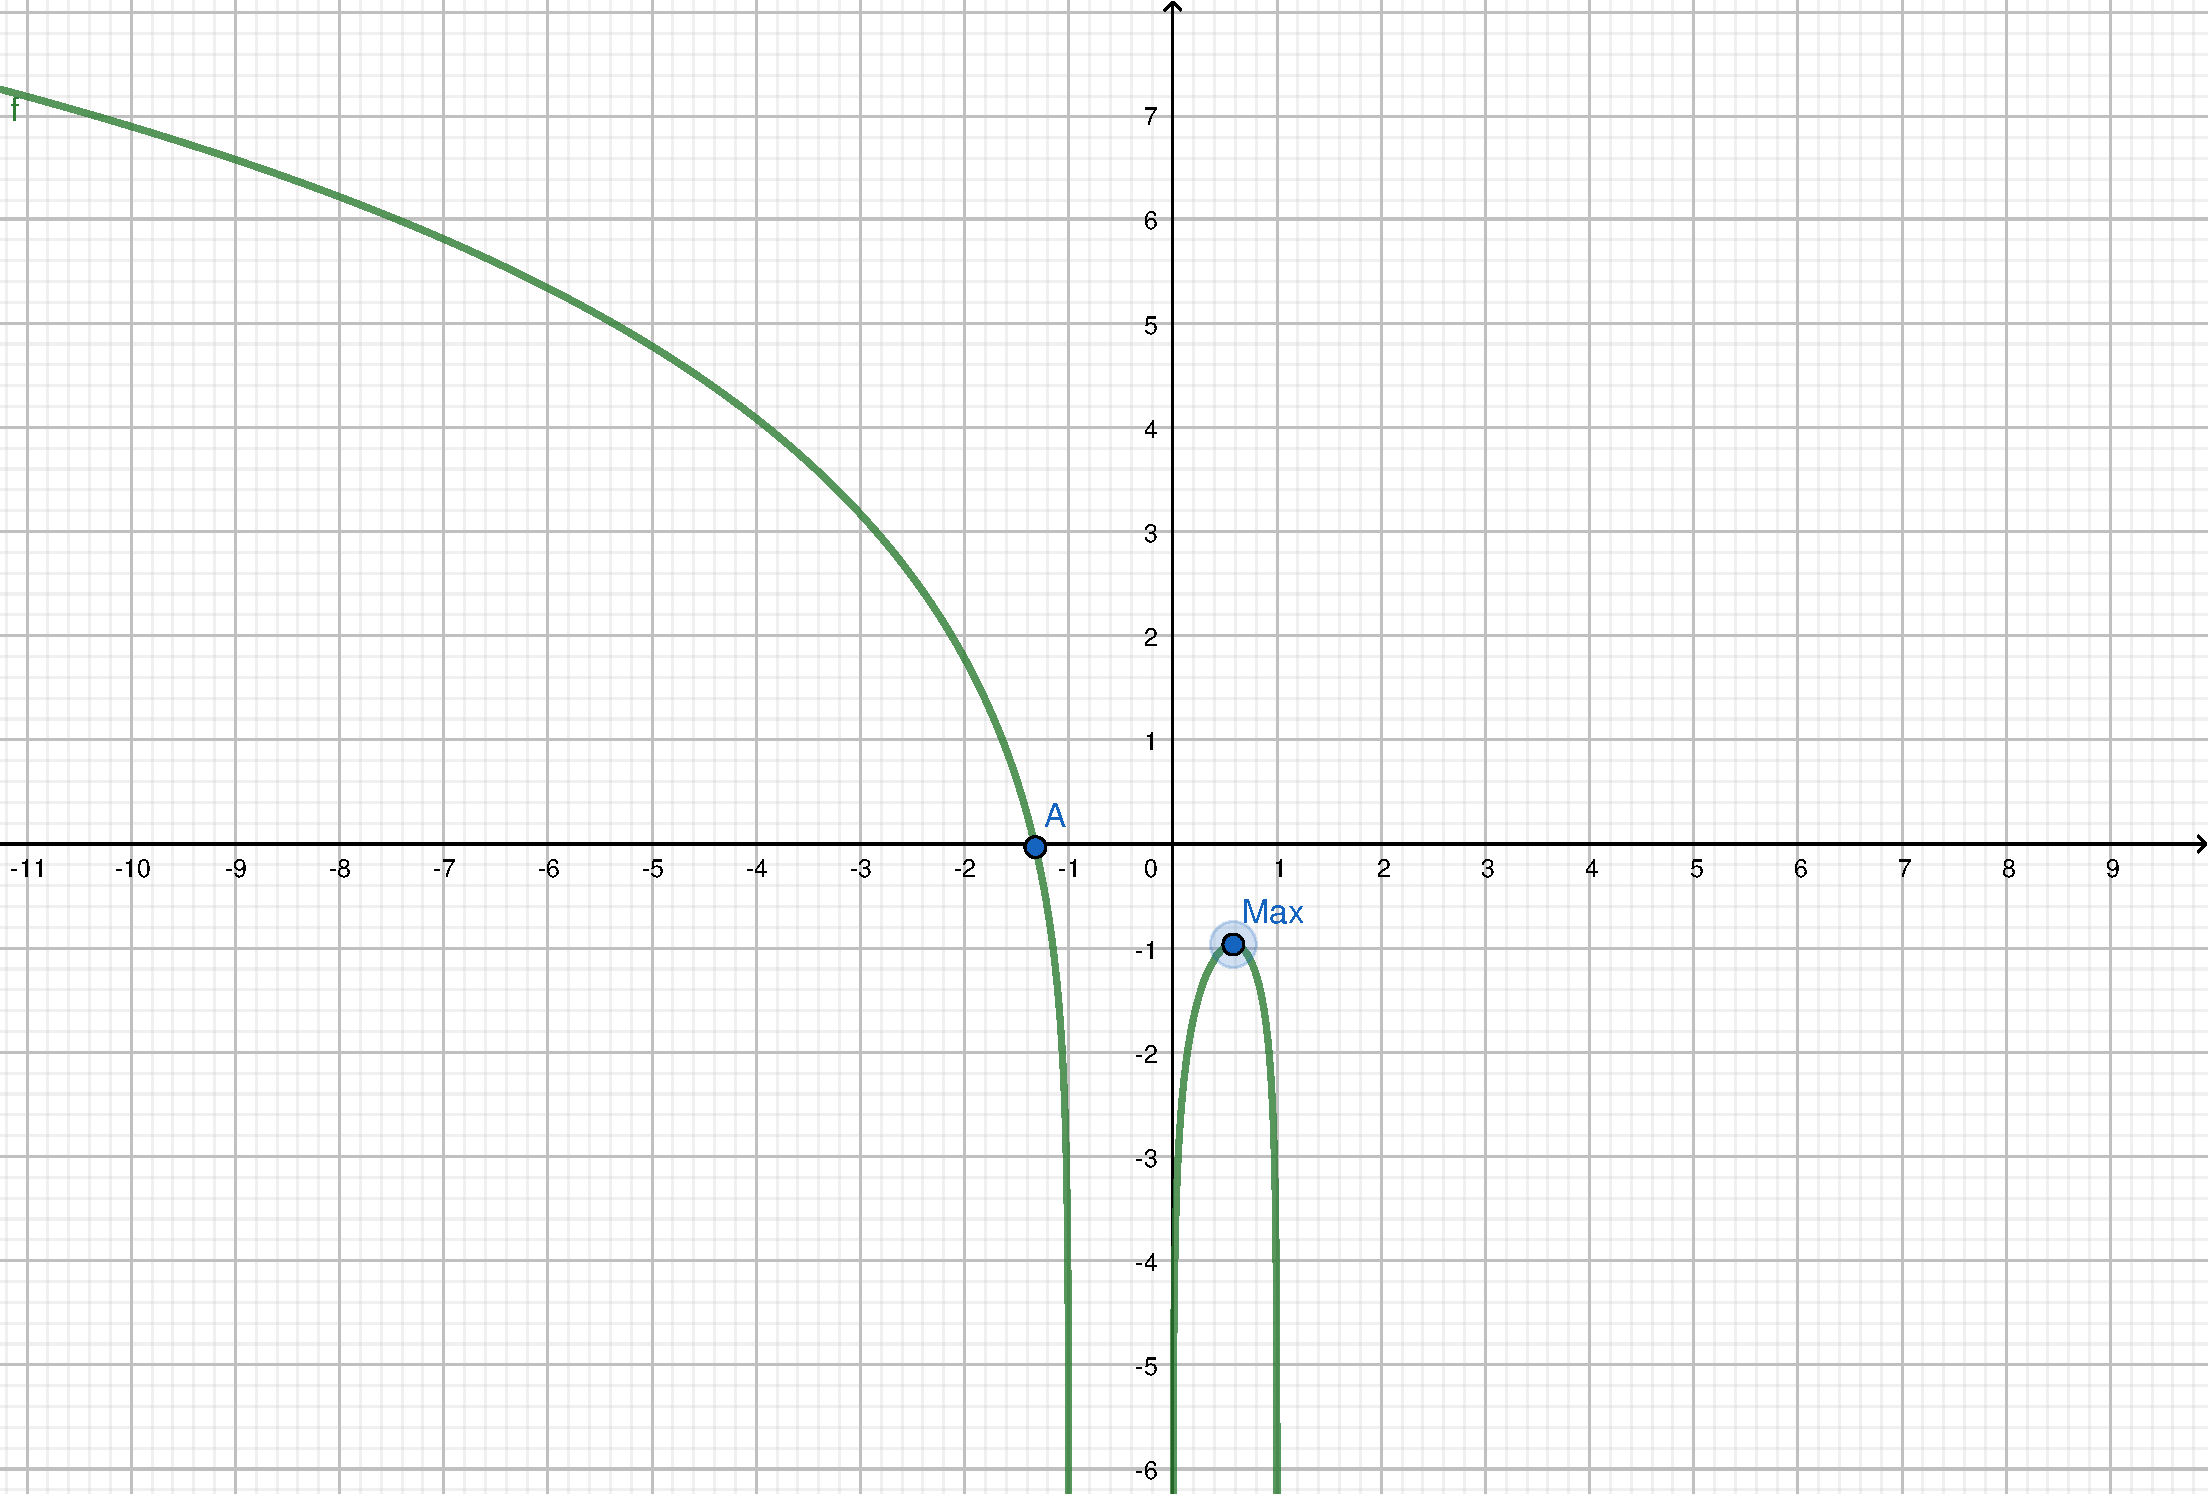
\includegraphics[height=8cm]{img/esercitazioni/esercitazione 1.pdf}};
		\end{tikzpicture}
		\caption{Grafico di Funzione $f(x)=\ln\left(x-x^3\right)$}
	\end{figure}
\end{enumerate}\newpage
\section{Integrali indefiniti}
\subsection{esercitazione 1}
	\begin{equation}
		\begin{matrix}
			\int e^{-3x}dx=-\frac{1}{3}e^{-3x}+C \\
			F(x)=-\frac{1}{3}e^{-3x}+C \\
			f(x)=e^{-3x}\\
			F^\prime(x)=-\frac{1}{3}*e^{-3x}*(-3)=e^{-3x}=f(x)
		\end{matrix}
	\end{equation}
\subsection{esercitazione 2}
	\begin{equation}
		\begin{matrix}
			\int x*e^{2x}dx\\
			\frac{1}{2}e^{2x}*x-\int\frac{1}{2}e^{2x}*1dx\\
			\frac{1}{2}e^{2x}*x-\frac{1}{2}\inf e^{2x}dx \\
			\frac{1}{2}e^{2x}*x-\frac{1}{2}*\frac{1}{2}e^{2x}+C\\
			\frac{1}{2}e^{2x}*\left( x-\frac{1}{2}\right)+C
		\end{matrix}
	\end{equation}
\subsection{esercitazione 3}
	\begin{equation}
		\begin{matrix}
			\int x^2dx=\frac{1}{3}x^3+C\\
			f(x)=x^2\\
			F(x)=\frac{1}{3}x^3+C\\
			D\left(\frac{1}{3}x^3+C\right)=\frac{1}{3}*3x^2=x^2
		\end{matrix}
	\end{equation}
\subsection{esercitazione 4}
	\begin{equation}
		\begin{matrix}
			\int \frac{1}{x}dx=\ln\left|x\right|+C\\
			\text{Dimostrazione}\\
			\ln\left|x\right|=\begin{cases}
					\ln x & \text{ se x > 0}\\
					\ln -x & \text{ se x < 0}
			\end{cases}\\
			D\ln\left|x\right|=\begin{cases}
				\frac{1}{x}\\
				\frac{1}{-x}*(-1)=\frac{1}{x}
			\end{cases}
		\end{matrix}
	\end{equation}
\subsection{esercitazione 5}
	\begin{equation}
		\begin{matrix}
			\int \frac{2x}{x^2+5}dx=\ln\left|x^2+5\right|+C
		\end{matrix}
	\end{equation}
\subsection{esercitazione 6}
	\begin{equation}
		\begin{matrix}
			\int \frac{3x^2}{x^2+1}dx=\ln\left|x^2+5\right|+C
		\end{matrix}
	\end{equation}
\subsection{esercitazione 7}
	\begin{equation}
		\begin{matrix}
			\int \frac{1}{y}dx=\ln y+C\\
			=\int \frac{1}{y^3}dy=\int y^{-3}dx\\
			=\int \frac{1}{-3+1}y^{-3+1}+C\\
			=-\frac{1}{2}y^{-2}+C\\
			=-\frac{1}{2y^2}+C
		\end{matrix}
	\end{equation}
\subsection{esercitazione 8}
	\begin{equation}
		\begin{matrix}
			\int \frac{1}{\sqrt{y}}dy\\
			\int
			y^{\frac{1}{2}}dy=\frac{1}{-\frac{1}{2}+1}y^{-\frac{1}{2}+1}+C\\
			=\frac{1}{\frac{1}{2}}y^\frac{1}{2}+C=2\sqrt{y}+C
		\end{matrix}
	\end{equation}
\subsection{esercitazione 9}
	\begin{equation}
		\begin{matrix}
			\int \frac{1}{\sqrt[3]{y}}dy=\int y^{-\frac{1}{3}}dy\\
			=\frac{1}{-\frac{1}{3}+1}y^{\frac{1}{3}+1}+C\\
			=\frac{1}{\frac{2}{3}}*y^{\frac{2}{3}}+C\\
			=\frac{3}{2}\sqrt[3]{y^2}+C\\
			-\frac{1}{3}+1=\frac{-1+3}{3}=\frac{2}{3}
		\end{matrix}
	\end{equation}
\subsection{esercitazione 10}
	\begin{equation}
		\begin{matrix}
			\int \sqrt[3]{y^2}dy=\int y^{\frac{2}{3}}dy\\
			=\frac{1}{\frac{2}{3}+1}y^{\frac{2}{3}+1}dy\\
			=\frac{1}{\frac{2+3}{3}}y^{\frac{2+3}{3}}dy\\
			=\frac{1}{\frac{5}{3}}y^{\frac{5}{3}}\\
			=\frac{3}{5}y^\frac{5}{3}\\
			=\frac{3}{5}\sqrt[3]{y^5}
		\end{matrix}
	\end{equation}
\subsection{esercitazione 11}
	\begin{equation}
		\begin{matrix}
			\int \sqrt[3]{y^2}\,dy=\int
			y^{\frac{2}{3}}dy\\
			=\frac{1}{\frac{2}{3}+1}y^{\frac{2}{3}+1}dy+C\\
			=\frac{1}{\frac{5}{3}}y^{\frac{5}{3}}+C\\
			=\frac{3}{5}\sqrt[3]{y^5}+C
		\end{matrix}
	\end{equation}
\section{Integrali definiti}
\subsection{Esercitazione 1}
	\begin{equation}
		\begin{matrix}
			\int_{1}^{3} \frac{x+1}{x+2}\,dx\\
			\left[x-\ln\abs{x+2}\right]_{1}^{3}\\
			=[3-\ln 5]-[1-\ln 3]\\
			=3-\ln 5-1+\ln 3\\
			=2+\ln\frac{3}{5}
		\end{matrix}
	\end{equation}
\subsection{Esercitazione 2}
	\begin{equation}
		\begin{matrix}
			\int_{1}^{3} \frac{x+1}{x+2}\,dx\\
			\int \frac{x+1+1-1{x+2}}\,dx\\
			=\int \frac{(x+2)+1}{x+2}\,dx\\
			=\int \frac{x+2}{x+2}\,dx-\int \frac{1}{x+2}\,dx\\
			=\int 2\,dx-\int\frac{1}{x+2}\,dx\\
			=x-\ln\abs{x+2}\\
			\left[x-\ln\abs{x+2}\right]_{1}^{3}\\
			=[3-\ln 5]-[1-\ln 3]\\
			=3-\ln 5-1+\ln 3\\
			=2+\ln\frac{3}{5}
		\end{matrix}
	\end{equation}
\section{Equazioni differenziali}
\subsection{Esercitazione 1}
	\begin{equation}
		\begin{matrix}
			y^\prime=y*x\\
			\frac{dy}{dx}=y*x\,dx\\
			dy=y*xdx\\
			\frac{dx}{y}=x*dx\\
			\int\frac{1}{y}=\int x\,dx\\
			\ln y=\frac{1}{2}x^2+C\\
			y=e^{\frac{1}{2}x^2+C}\\
			y=e^{\frac{1}{2}x^2}*e^c\\
			y=k*e^{\frac{1}{2}x^2}
		\end{matrix}
	\end{equation}



\printindex
\end{document}
